% Options for packages loaded elsewhere
% Options for packages loaded elsewhere
\PassOptionsToPackage{unicode}{hyperref}
\PassOptionsToPackage{hyphens}{url}
%
\documentclass[
  spanish,
  11pt,
  a4paper,
]{scrbook}
\usepackage{xcolor}
\usepackage[left=3cm,right=3cm,top=3cm,bottom=4cm]{geometry}
\usepackage{amsmath,amssymb}
\setcounter{secnumdepth}{-\maxdimen} % remove section numbering
\usepackage{iftex}
\ifPDFTeX
  \usepackage[T1]{fontenc}
  \usepackage[utf8]{inputenc}
  \usepackage{textcomp} % provide euro and other symbols
\else % if luatex or xetex
  \usepackage{unicode-math} % this also loads fontspec
  \defaultfontfeatures{Scale=MatchLowercase}
  \defaultfontfeatures[\rmfamily]{Ligatures=TeX,Scale=1}
\fi
\usepackage{lmodern}
\ifPDFTeX\else
  % xetex/luatex font selection
  \setmainfont[]{Cormorant Garamond}
\fi
% Use upquote if available, for straight quotes in verbatim environments
\IfFileExists{upquote.sty}{\usepackage{upquote}}{}
\IfFileExists{microtype.sty}{% use microtype if available
  \usepackage[]{microtype}
  \UseMicrotypeSet[protrusion]{basicmath} % disable protrusion for tt fonts
}{}
\makeatletter
\@ifundefined{KOMAClassName}{% if non-KOMA class
  \IfFileExists{parskip.sty}{%
    \usepackage{parskip}
  }{% else
    \setlength{\parindent}{0pt}
    \setlength{\parskip}{6pt plus 2pt minus 1pt}}
}{% if KOMA class
  \KOMAoptions{parskip=half}}
\makeatother
% Make \paragraph and \subparagraph free-standing
\makeatletter
\ifx\paragraph\undefined\else
  \let\oldparagraph\paragraph
  \renewcommand{\paragraph}{
    \@ifstar
      \xxxParagraphStar
      \xxxParagraphNoStar
  }
  \newcommand{\xxxParagraphStar}[1]{\oldparagraph*{#1}\mbox{}}
  \newcommand{\xxxParagraphNoStar}[1]{\oldparagraph{#1}\mbox{}}
\fi
\ifx\subparagraph\undefined\else
  \let\oldsubparagraph\subparagraph
  \renewcommand{\subparagraph}{
    \@ifstar
      \xxxSubParagraphStar
      \xxxSubParagraphNoStar
  }
  \newcommand{\xxxSubParagraphStar}[1]{\oldsubparagraph*{#1}\mbox{}}
  \newcommand{\xxxSubParagraphNoStar}[1]{\oldsubparagraph{#1}\mbox{}}
\fi
\makeatother


\usepackage{longtable,booktabs,array}
\newcounter{none} % for unnumbered tables
\usepackage{calc} % for calculating minipage widths
% Correct order of tables after \paragraph or \subparagraph
\usepackage{etoolbox}
\makeatletter
\patchcmd\longtable{\par}{\if@noskipsec\mbox{}\fi\par}{}{}
\makeatother
% Allow footnotes in longtable head/foot
\IfFileExists{footnotehyper.sty}{\usepackage{footnotehyper}}{\usepackage{footnote}}
\makesavenoteenv{longtable}
\usepackage{graphicx}
\makeatletter
\newsavebox\pandoc@box
\newcommand*\pandocbounded[1]{% scales image to fit in text height/width
  \sbox\pandoc@box{#1}%
  \Gscale@div\@tempa{\textheight}{\dimexpr\ht\pandoc@box+\dp\pandoc@box\relax}%
  \Gscale@div\@tempb{\linewidth}{\wd\pandoc@box}%
  \ifdim\@tempb\p@<\@tempa\p@\let\@tempa\@tempb\fi% select the smaller of both
  \ifdim\@tempa\p@<\p@\scalebox{\@tempa}{\usebox\pandoc@box}%
  \else\usebox{\pandoc@box}%
  \fi%
}
% Set default figure placement to htbp
\def\fps@figure{htbp}
\makeatother

\ifLuaTeX
  \usepackage{luacolor}
  \usepackage[soul]{lua-ul}
\else
  \usepackage{soul}
\fi


\ifLuaTeX
\usepackage[bidi=basic,shorthands=off]{babel}
\else
\usepackage[bidi=default,shorthands=off]{babel}
\fi
\ifPDFTeX
\else
\babelfont{rm}[]{Cormorant Garamond}
\fi
\ifLuaTeX
  \usepackage{selnolig} % disable illegal ligatures
\fi


\setlength{\emergencystretch}{3em} % prevent overfull lines

\providecommand{\tightlist}{%
  \setlength{\itemsep}{0pt}\setlength{\parskip}{0pt}}



 
\usepackage[refsection=chapter,style=apa,isbn=false]{biblatex}
\addbibresource{Libro.bib}


% ==============================================================================
% CONFIGURACIÓN GLOBAL DEL LIBRO (Unificación Definitiva - Libro 1)
% ==============================================================================

% --- 1. Fuentes y Tipografía Replicables (Solución Física Mac) ---
\usepackage{fontspec}
\setmainfont{Cormorant Garamond}[
    UprightFont = *-Medium
]
\setsansfont{Montserrat-Regular.otf}[
    BoldFont = Montserrat-SemiBold.otf
]

% --- 2. Ajustes de Párrafo y Espaciado Vertical (Estilo Refinado) ---
\usepackage{widows-and-orphans}
\widowpenalty=10000
\clubpenalty=10000
\setlength{\parindent}{1.2em} % Sangría de primera línea ganadora
\setlength{\parskip}{0pt}     % Sin espacios vacíos entre párrafos ordinarios

\usepackage{setspace}
\setstretch{1.3}              % Interlineado sofisticado y compacto

% --- 3. Jerarquía y Alineación de Títulos (KOMA-Script) ---
\addtokomafont{disposition}{\sffamily\fontspec{Montserrat-SemiBold.otf}}
\addtokomafont{chapter}{\huge\raggedright}
\addtokomafont{section}{\Large\raggedright}
\addtokomafont{subsection}{\normalsize}

% --- 4. Encabezados y Pies de Página (Mantenido de tu estructura) ---
\usepackage{scrlayer-scrpage}
\automark{chapter}

% --- 5. Gestión de Gráficos e Imágenes ---
\usepackage{graphicx}
\graphicspath{{../assets/imagenes/}{../../institucionales/assets/logos/}}

% --- 6. Ajustes Finos de Disposición de Capítulos ---
\addtokomafont{disposition}{\linespread{1.2}\selectfont}
\RedeclareSectionCommand[
    beforeskip=-0.0cm,
    afterskip=1.5cm
]{chapter}

% ==============================================================================
% CONFIGURACIÓN DE IDIOMA Y CONECTORES PARA BIBLATEX (ESTILO APA)
% ==============================================================================

% 1. Definir las cadenas de traducción oficiales al español
\DefineBibliographyStrings{spanish}{%
  and = {y},
  andothers = {et~al.},
  volume = {vol.},
  volumes = {vols.},
  pages = {pp.},
  page = {p.}
}

% 2. Forzar al estilo APA a usar la "y" en lugar del ampersand (&) en los textos e índices
\DeclareDelimFormat*{finalnamedelim}{\addspace\bibstring{and}\addspace}
\DeclareDelimFormat*{finalnamedelim:apaenum}{\addspace\bibstring{and}\addspace}
% ==============================================================================
% ENSTORNOS Y COMANDOS PERSONALIZADOS (Especial para Etnografía y Entrevistas)
% ==============================================================================

% --- 1. Paquetes requeridos para control de listas y color ---
\usepackage{enumitem}
\usepackage{xcolor}

% --- 2. Entorno para transcripciones de entrevistas estructuradas ---
% Corrige espaciados para que los fragmentos no queden flotando o muy separados
\newenvironment{transcripcion}{
    \begin{list}{}{
        \setlength{\leftmargin}{1.5em}  % Un toque más de entrada para notar el bloque
        \setlength{\rightmargin}{0em}
        \setlength{\itemsep}{0.2em}     % Ajuste fino de separación entre réplicas
        \setlength{\parsep}{0.0em}
        \setlength{\listparindent}{0pt}
    }
}{
    \end{list}
}

% --- 3. Comandos auxiliares para dinamismo de diálogos etnográficos ---
% \personaje{Nombre}: Renderiza el actor social en negrita con un espacio elegante
\newcommand{\personaje}[1]{\textbf{#1}\quad}

% \escena{Texto}: Ideal para descripciones de diario de campo o gestos en cursiva y chica
\newcommand{\escena}[1]{\textit{\small #1}\par\vspace{0.4em}}
\makeatletter
\@ifpackageloaded{bookmark}{}{\usepackage{bookmark}}
\makeatother
\makeatletter
\@ifpackageloaded{caption}{}{\usepackage{caption}}
\AtBeginDocument{%
\ifdefined\contentsname
  \renewcommand*\contentsname{Tabla de contenidos}
\else
  \newcommand\contentsname{Tabla de contenidos}
\fi
\ifdefined\listfigurename
  \renewcommand*\listfigurename{Listado de Figuras}
\else
  \newcommand\listfigurename{Listado de Figuras}
\fi
\ifdefined\listtablename
  \renewcommand*\listtablename{Listado de Tablas}
\else
  \newcommand\listtablename{Listado de Tablas}
\fi
\ifdefined\figurename
  \renewcommand*\figurename{Figura}
\else
  \newcommand\figurename{Figura}
\fi
\ifdefined\tablename
  \renewcommand*\tablename{Tabla}
\else
  \newcommand\tablename{Tabla}
\fi
}
\@ifpackageloaded{float}{}{\usepackage{float}}
\floatstyle{ruled}
\@ifundefined{c@chapter}{\newfloat{codelisting}{h}{lop}}{\newfloat{codelisting}{h}{lop}[chapter]}
\floatname{codelisting}{Listado}
\newcommand*\listoflistings{\listof{codelisting}{Listado de Listados}}
\makeatother
\makeatletter
\makeatother
\makeatletter
\@ifpackageloaded{caption}{}{\usepackage{caption}}
\@ifpackageloaded{subcaption}{}{\usepackage{subcaption}}
\makeatother
\usepackage{bookmark}
\IfFileExists{xurl.sty}{\usepackage{xurl}}{} % add URL line breaks if available
\urlstyle{same}
% fallback for those not using the hyperref driver hyperxmp:
\makeatletter
\@ifundefined{xmpquote}{\newcommand{\xmpquote}[1]{#1}}{}
\makeatother
\hypersetup{
  pdftitle={Experimentación Formal en Internet o de cómo las Ciencias Sociales habitan la galaxia},
  pdflang={es},
  hidelinks,
  pdfcreator={LaTeX via pandoc}}


\title{Experimentación Formal en Internet o de cómo las Ciencias
Sociales habitan la galaxia}
\usepackage{etoolbox}
\makeatletter
\providecommand{\subtitle}[1]{% add subtitle to \maketitle
  \apptocmd{\@title}{\par {\large #1 \par}}{}{}
}
\makeatother
\subtitle{Convergencias, algoritmos y narrativas emergentes}
\author{}
\date{2026-09-07}
\begin{document}
\frontmatter
\maketitle

% ============================================
% DEFINICIÓN DE FUENTE PARA LA PORTADA
% ============================================
\newfontfamily\montserrat[
  Path=assets/fuentes/Montserrat/static/,
  Extension=.ttf,
  BoldFont=Montserrat-SemiBold,
  ItalicFont=Montserrat-Italic  % Si no existe, fontspec usará slant sintético
]{Montserrat-Regular}


%=============================================================================
% PÁGINA 1: PORTADA FULL-PAGE
%=============================================================================
{ % <--- LLAVE DE APERTURA (Blindaje total de márgenes)

\thispagestyle{empty}

\hoffset=-1in
\voffset=-1in
\oddsidemargin=0pt
\evensidemargin=0pt
\topmargin=0pt
\headheight=0pt
\headsep=0pt

\noindent
% El comando \lower agarra la caja de ancho cero y la desplaza hacia abajo de forma obligatoria.
% Empezamos con 1.8cm. Si notas que le falta bajar un poco, súbelo a 2.5cm.
\lower 1.8cm \hbox to \paperwidth{%
    \hss
    \includegraphics[width=\paperwidth,height=1.0\paperheight,keepaspectratio=false]{assets/imagenes/libro1portada2026.pdf}%
    \hss
}

\clearpage

} % <--- LLAVE DE CIERRE (Márgenes del libro restaurados automáticamente)
% ============================================
% PÁGINA 2: EN BLANCO (verso de portada)
% ============================================
\clearpage
\thispagestyle{empty}
\null
\clearpage
% ============================================
% PÁGINA 3: PORTADILLA (MEDIA PORTADA)
% ============================================
\clearpage
  \thispagestyle{empty}
  \begingroup
    \raggedright
    \vspace*{1cm}
    \sffamily\small
    \montserrat\huge Experimentación formal en internet \\ o de cómo las ciencias sociales habitan la galaxia \\
    \vspace{0.3cm}
    {\Large Convergencias, algoritmos y narrativas emergentes} \\
    \vspace{0.7cm}
    {\Large Fernando Rodrigo Beltrán Nieves} \\
    \vspace{0.3cm}
    \Large\rmfamily\textit{Coordinador}
    \vfill
  % Centrado exacto de la imagen
  \begin{center}
    
\includegraphics[width=0.4\textwidth]{../../assets/logos/logoUAML.png}
  \end{center}
  
  \vspace{1cm} % Espacio de respiro antes del corte de página
  \endgroup
\clearpage


% ==============================================================================
% PÁGINA 4: DIRECTORIO INSTITUCIONAL CENTRADO
% ==============================================================================
\clearpage
  \begingroup
    \thispagestyle{empty}
      \begin{center}
        \sffamily\small
        {\montserrat\Large\textbf{UNIVERSIDAD AUTÓNOMA METROPOLITANA}} \\
        {\montserrat\large\textbf{RECTORÍA GENERAL}} \\
        \vspace{0.2cm}
        \textit{Dr. Raúl Gustavo Pacheco López} \\
        Rector \\
        \vspace{0.1cm}
        {\itshape Dra. Esthela Irene Sotelo Núñez} \\
        Secretaria General\\
        
        \vspace{0.1cm}
        \rule{0.6\textwidth}{0.4pt}
        \vspace{0.1cm}
        
        {\montserrat\large\textbf{UNIDAD LERMA}} \\
        \vspace{0.2cm}
        \textit{Dra. Alma Patricia de León Calderón} \\
        Rectora \\
        \vspace{0.1cm}
        {\itshape Dra. Karla Pelz Serrano} \\
        Secretaria \\
        \vspace{0.1cm}
        {\montserrat\large\textbf{División de Ciencias Sociales y Humanidades}} \\
        \vspace{0.1cm}
        \textit{Dr. Raúl Hernández Mar} \\
        Director \\
        \vspace{0.1cm}
        \textit{Dra. Ana Carolina Robles Salvador} \\
        Secretaria Académica \\
  
        %\vspace{0.1cm}
        \rule{0.6\textwidth}{0.4pt}
        %\vspace{0.1cm}
  
        {\montserrat\large\textbf{Consejo Editorial - Publicaciones Periódicas}} \\
        %{\montserrat\normalfont{Publicaciones Periódicas}} \\
        \vspace{0.2cm}
        \textit{Abigail Martínez Mendoza} \\
        Coordinadora General \\
        \vspace{0.1cm}
        \textit{Omar Valencia Domínguez} \\
        \textit{Ryszard Edward Rozga Luter} \\
        Departamento de Procesos Sociales \\
        \vspace{0.1cm}
        \textit{José Omar Pérez Baños} \\
        Departamento de Estudios Culturales \\
        
        %\vspace{0.1cm}
        \rule{0.6\textwidth}{0.4pt}
        %\vspace{0.1cm}
        
        {\montserrat\large\textbf{Edición Técnica, Corrección de Estilo y Diseño}} \\
        \vspace{0.2cm}
        \textit{José Omar Pérez Baños} \\
        Director del Equipo Editorial \\
        \vspace{0.1cm}
        \textit{Jonathan Armando Chávez Solís} \\
        Editor Literario\\
        \textit{Yunuen Rosas Ortiz} \\
        Ilustradore \\
      \end{center}
  \endgroup
\clearpage

% ==============================================================================
% PÁGINA 5: PÁGINA LEGAL ESTÁNDAR (DCSH - UAM LERMA)
% ==============================================================================

\clearpage
\thispagestyle{empty}
\begin{center}
    % --- Ficha de Catalogación Superior ---
    \framebox[\textwidth]{\vbox{
        \vspace{0.3cm}
        \hbox to \textwidth{\hfill\montserrat\scriptsize\textbf DATOS DE CATALOGACIÓN\hfill}
        \vspace{0.2cm}
        \noindent\hspace{0.5cm}
        \parbox{0.9\textwidth}{
            \rmfamily\scriptsize
            \texttt{Beltrán Nieves, Fernando Rodrigo (coordinador)} \\
            Experimentación formal en internet o de cómo las Ciencias Sociales habitan la galaxia : Convergencias, algoritmos y narrativas emergentes / Fernando Rodrigo Beltrán Nieves, coordinador. -- México : Universidad Autónoma Metropolitana : Unidad Lerma : División de Ciencias Sociales y Humanidades, 2026. \\
            \quad p. : il. ; 14 x 21 cm. \\
            \quad ISBN: 978-xxx-xxx-xxx-x \\
            \quad 1. Internet -- Aspectos sociales. 2. Innovaciones tecnológicas -- Aspectos sociales. 3. Sociología de la comunicación. 4. Algoritmos -- Aspectos sociales. 5. Podcasting en la educación superior. 6. Ciencias sociales -- Metodología. 
-- México. I. Universidad Autónoma Metropolitana. Unidad Lerma. División de Ciencias Sociales y Humanidades.
        }
        \vspace{0.3cm}
    }}
\end{center}

\vspace*{\fill} % Empuja los datos legales al fondo de la página

% --- Créditos y Derechos de Autor ---

\begingroup
\begin{singlespace}
\fontspec{Montserrat-Regular.otf}\scriptsize
\noindent
Primera edición: 2026\\
Experimentación Formal en Internet o de cómo las Ciencias Sociales habitan la galaxia: Convergencias, algoritmos y narrativas emergentes\\
Fernando Rodrigo Beltrán Nieves, coordinador\\[0.5em]
Diseño de portada: Yunuen Rosas Ortiz\\[0.5em]
D.R. © 2026, Universidad Autónoma Metropolitana\\
Prolongación Canal de Miramontes 3855, Ex Hacienda San Juan de Dios,\\
Alcaldía de Tlalpan, C.P. 14387, Ciudad de México.\\[0.5em]
{\fontspec{Montserrat-SemiBold.otf}\scriptsize Universidad Autónoma Metropolitana, Unidad Lerma}\\
División de Ciencias Sociales y Humanidades\\
Consejo Editorial de la División de Ciencias Sociales y Humanidades\\
Avenida de las Garzas núm. 10, Col. El Panteón,\\
C.P. 52005, Lerma de Villada, Estado de México.\\
Contacto: \href{mailto:cedcsh@correo.ler.uam.mx}{cedcsh@correo.ler.uam.mx}\\[0.8em]
ISBN: 978-xxx-xxx-xxx-x\\[0.8em]
Esta publicación no puede ser reproducida, ni en todo ni en parte, ni registrada o transmitida por un sistema de recuperación de información, en ninguna forma ni por ningún medio, sea mecánico, fotoquímico, electrónico, magnético, electroóptico, por fotocopia o cualquier otro, sin el permiso previo y por escrito de los editores.\\[0.5em]
La presente publicación pasó por un proceso de dos dictámenes (doble ciego) de pares académicos avalados por el Consejo Editorial de la División de Ciencias Sociales y Humanidades de la UAM-Lerma, que garantizan su calidad y pertinencia académica y científica.\\[0.5em]
Publicación digital hecha en México / Digital publication made in Mexico
\end{singlespace}
\endgroup
\clearpage

% ============================================
% PÁGINA EN BLANCO
% ============================================
\clearpage
\thispagestyle{empty}
\null
\clearpage

\renewcommand*\contentsname{Índice}
{
\setcounter{tocdepth}{1}
\tableofcontents
}

\mainmatter
\bookmarksetup{startatroot}

\chapter*{INTRODUCCIÓN}\label{introducciuxf3n}
\addcontentsline{toc}{chapter}{INTRODUCCIÓN}

\markboth{INTRODUCCIÓN}{INTRODUCCIÓN}

\vspace{-\baselineskip}

\addtocontents{toc}{\protect\hspace{1.5em}Fernando Rodrigo Beltrán Nieves\par}

La relación entre las Ciencias Sociales y la galaxia internet ha dejado
de ser un objeto de estudio para convertirse en un espacio de
reconfiguración epistemológica, metodológica y política. Los cinco
capítulos de investigación aquí reunidos: ``Capitalismo cognitivo,
gubernamentalidad algorítmica y abordajes de la comunicación'' de Miguel
Ángel Mata Salazar; ``Hegemonía algorítmica y visibilidad académica. Una
propuesta metodológica'' de Christian Hernández Pérez; ``Nuevas formas
de narrar la realidad. El proceso de individuación y su impacto en la
escritura académica'' de Paola Vázquez Almanza; ``Ensayo sobre un
pódcast de investigación sociológica'' de Fernando Beltrán Nieves; y
``El podcasting como herramienta tecnopedagógica en la construcción de
una narrativa transmedia: el caso Versátil'' de Diego Valdez Serrano,
dialogan entre sí desde distintas aristas de un mismo fenómeno: la
transformación radical de la producción, circulación y legitimación del
conocimiento en las revoluciones permanentes que sufre internet.

Capitalismo cognitivo y algoritmos: el nuevo régimen de visibilidad. El
primer trabajo de este libro colectivo, Capitalismo cognitivo,
gubernamentalidad algorítmica y abordajes de la comunicación, establece
un marco teórico indispensable al vincular el capitalismo cognitivo con
la gubernamentalidad algorítmica, mostrando cómo las lógicas de
acumulación y control se rearticulan en la digitalidad. Esta perspectiva
encuentra un eco empírico en el segundo artículo, Hegemonía algorítmica
y visibilidad académica, que analiza cómo los algoritmos de Google
condicionan la visibilidad de los académicos en México.

Mientras el primero teoriza sobre el poder estructurante de las
plataformas, el segundo lo operacionaliza, revelando un conflicto
central: en un mundo donde la relevancia académica se mide en clics y
posicionamiento, ¿qué sucede con las Ciencias Sociales y Humanidades
críticas, tradicionalmente alejadas de las métricas virales? Ambos
textos convergen en señalar que la academia no es ajena a la
mercantilización de la atención ni a la dataficación de sus prácticas.
Narrativas en transición: de la escritura tradicional al giro sonoro. El
tercer artículo de este número, Nuevas formas de narrar la realidad,
introduce un giro crucial al cuestionar las formas canónicas de
escritura académica, abogando por una mayor imbricación entre
experiencia individual y divulgación. Esta preocupación por democratizar
el conocimiento se materializa en los dos trabajos restantes, dedicados,
ambos, al pódcast. El Ensayo sobre un pódcast de investigación
sociológica analiza las posibilidades analíticas de la sociología en un
medio sonoro, mientras que el segundo artículo, El podcasting como
herramienta tecnopedagógica en la construcción de una narrativa
transmedia: el caso Versátil, explora el formato como herramienta
didáctica en expansión en los recintos universitarios. Los tres textos
comparten una hipótesis implícita: la rigidez de los formatos académicos
tradicionales limita su impacto social, mientras que las narrativas
transmedia ---especialmente el audio--- permiten una circulación ágil y
una apropiación colectiva del saber. Por lo demás, el Ensayo sobre un
pódcast de investigación sociológica explora la técnica de la
interrupción como recurso narrativo, proponiendo un ejercicio
contrafactual sobre Karl Marx que desafía los límites entre ficción y
análisis social. Por su parte, el estudio del pódcast Versátil muestra
cómo este formato se ha convertido en un puente entre la universidad y
el espacio público, siempre que se superen barreras institucionales.
Aquí, la compatibilidad de la obra colectiva es evidente: si el
capitalismo cognitivo convierte el conocimiento en commodity, como lo
señala el trabajo de Miguel Ángel Mata, estas iniciativas académicas en
el audio, por el contrario, buscan subvertir esa lógica mediante
prácticas colaborativas y accesibles. Tensiones y desafíos: ¿hacia una
ciencia social expandida?

La relevancia de este esfuerzo académico colectivo radica en su
capacidad para mapear las tensiones contemporáneas de las Ciencias
Sociales en la galaxia internet: desde la dependencia de
infraestructuras algorítmicas privadas hasta la experimentación con
formatos que desafían el paper como único vehículo legítimo. Los cinco
textos, en conjunto, trazan un diagnóstico y una ruta de acción. En
efecto, efectúan colectivamente una crítica sustantiva al denunciar la
subsunción de lo académico bajo racionalidades tecnoliberales
(algoritmos, métricas, plataformas), pero también apuestan por
narrativas emergentes (podcasts, técnicas de interrupción, transmedia)
que reconfiguren la relación entre investigadores y audiencias. Una
crítica frontal al explorar y proponer una suerte de innovación táctica.

Quedan preguntas abiertas. ¿Cómo evitar que la ``visibilidad'' en
internet reproduzca desigualdades ya existentes o, peor aún, las
profundice? ¿Pueden los formatos sonoros eludir la mercantilización que
critica el primer artículo? Lo cierto es que, como lo muestran estos
capítulos de investigación, las Ciencias Sociales están obligadas a
navegar ---y transformar--- el ecosistema digital, so pena de volverse
irrelevantes. Esta colección no sólo aporta claves para ese viaje, sino
que lo ejemplifica, plasmando rigor teórico, metodologías audaces y un
compromiso con la circulación plural del conocimiento. En última
instancia, estos textos son artefactos de una misma constelación: la que
busca repensar la academia desde sus fisuras, allí donde internet
desordena jerarquías y obliga a reinventar lo posible.

Coronamos este libro, por último, con una reseña crítica de Sandra
Isabella Carrillo Cima sobre Todos los museos son novelas de ciencia
ficción del crítico catalán Jorge Carrión. Un trabajo de lectura atenta
por parte de Carrillo Cima sobre las escrituras narrativas en atención a
la expansión inexorable de la inteligencia artificial, una más de las
revoluciones que sufre la galaxia internet.

\begin{flushright}
\Large Fernando Beltrán Nieves\\

\Large \textit{Coordinador}
\end{flushright}

\part{CONVERGENCIAS, ALGORITMOS Y NARRATIVAS EMERGENTES}

\chapter{Capitalismo cognitivo, gubernamentalidad algorítmica y
abordajes de la
comunicación}\label{capitalismo-cognitivo-gubernamentalidad-algoruxedtmica-y-abordajes-de-la-comunicaciuxf3n}

\addtocontents{toc}{\protect\hspace{1.5em}Miguel Ángel Mata Salazar\par}
\markboth{Capitalismo Cognitivo}{}

\begin{flushright}
\Large Miguel Ángel Mata Salazar \footnote{Facultad de Estudios Superiores Aragón, UNAM. Contacto: \href{anomjo@yaho.com.mx}{anomjo@yaho.com.mx}}
\end{flushright}

\section*{Introducción. Fases Históricas del
capitalismo}\label{introducciuxf3n.-fases-histuxf3ricas-del-capitalismo}

\markright{Introducción. Fases Históricas del capitalismo}

Como resultado de una revolución tecnológica el capitalismo ha
transitado históricamente por una fase mercantil e industrial. De ahí
que, ante el impacto que en las últimas décadas han tenido en el mundo
las Tecnologías de Información y Comunicación, este hecho resulte
indicativo de la transición hacia una nueva fase: el capitalismo
cognitivo, con el cual se despliega una nueva forma de producción,
identificable por el crecimiento sectorial de actividad y productos en
base a la ciencia, el conocimiento y la comunicación como fuerza
productiva para la acumulación de capital \autocite{Ordonez2011}.

El desarrollo teórico del capitalismo cognitivo surge en Francia con la
revista Multitudes a inicios del año 2000 \autocite[28]{Miguez2013},
publicación que se constituyó en un punto de confluencia de
intelectuales de distintas disciplinas y tradiciones de pensamiento que,
desde la década de los noventa, compartían afinidades respecto a los
debates en torno al ``Trabajo Inmaterial'' dentro del movimiento obrero
italiano, al obrerismo y la ``autonomía obrera''. Estas discusiones se
desarrollaron ante el incremento en la automatización de los procesos
productivos entre los años sesenta y setenta del siglo XX, ocupando la
atención dentro del capitalismo más avanzado, particularmente la planta
industrial de Italia, y generando una reinterpretación del marxismo para
su análisis.

Otra vertiente en la construcción teórica del capitalismo cognitivo es
la teoría de la regulación \autocite{Aglietta1979}, en la cual las
distintas etapas de la sociedad capitalista se han conformado de acuerdo
al régimen de acumulación y la forma en que se reguló cada fase,
identificando una relación compatible entre relaciones sociales e
instituciones para observar analíticamente el modo en que los patrones
de conducta sostienen o guían un régimen de acumulación de capital en un
cierto período. Por ello a partir de la década de los años setenta en
los países avanzados la automatización de la producción, la aplicación
de la electrónica y la informática en los procesos productivos se
consideran los principales indicadores de una nueva fase del
capitalismo.

Sin embargo, mientras temas como la automatización y los cambios en los
procesos de trabajo mantenían la atención en los estudiosos del tema, la
irrupción de la crisis del Estado de Bienestar, y la gradual presencia
de una revolución de las tecnologías de información y comunicación,
propiciaron la conformación de nuevos procesos productivos, vinculados
ahora al fenómeno de la globalización, mostrando, desde la perspectiva
de la crítica de la economía política, el vínculo de la tecnología con
la organización sociopolítica. De ahí que los argumentos centrales sobre
el capitalismo cognitivo se sustenten principalmente en las siguientes
obras de Karl Marx: el capítulo VI (inédito) del Libro I de \emph{El
capital}, titulado ``Resultados del proceso inmediato de producción'';
en la noción del ``\emph{General Intellect}'' de los \emph{Elementos
fundamentales para la crítica de la economía política (Grundrisse)
1857-1858}; y en \emph{El capital. Crítica de la economía política}.

\subsection*{Subsunción del trabajo al
capital}\label{subsunciuxf3n-del-trabajo-al-capital}

En El Capital Libro I Capítulo VI, \textcite{Marx2009inedito} analiza
los presupuestos del proceso de producción y valorización capitalista en
la que, como resultado del proceso inmediato de producción, el trabajo
productivo ha de ser trabajo asalariado del capital, condición histórica
con la cual ``el trabajo productivo debe producir valores de uso, y al
mismo tiempo, ser intercambiado por capital.''
\autocite[11]{Carcanholo2013}. De ahí que la subsunción implique
sometimiento del trabajo bajo el capital y su inclusión dentro de este
\autocite[XV]{Marx2009inedito}.

Los efectos de la profundización lógica, e histórica, de la subsunción
del proceso de trabajo definen al proceso de trabajo como una actividad
racional, encaminada a:

\begin{quote}
la producción de valores de uso, la asimilación de las materias
naturales al servicio de las necesidades humanas, la condición general
del intercambio de materias entre la naturaleza y el hombre, la
condición natural eterna de la vida humana, y por tanto, independiente
de las formas y modalidades de esta vida y común a todas las formas
sociales por igual \autocite[136]{Marx2009tomo1}.
\end{quote}

La subsunción implica un proceso de trabajo y un proceso de
valorización, en lo cual la mercancía es una porción de la naturaleza,
transformada por el capital en valor de uso y en valor de cambio
mediante el trabajo de un proceso productivo y en riqueza abstracta
genérica. La subsunción del trabajo al capital ha presentado dos etapas
y, con ellas, dos formas de plusvalía.

\subsection*{Subsunción formal del trabajo al
capital}\label{subsunciuxf3n-formal-del-trabajo-al-capital}

Es la etapa en la que los capitalistas organizan el trabajo en torno al
salario sin embargo, aún y cuando el taller se convierte en una empresa
capitalista y los artesanos en asalariados, no se modifica el proceso
laboral del taller artesanal, pues ``\ldots el capital ya existe
desempeñando determinadas funciones subordinadas, pero no aún en su
función dominante, determinante de la forma social general, en su
condición de comprador directo de trabajo y apropiador directo del
proceso de producción'' \autocite[57-58]{Marx2009inedito}. Esta fase
corresponde a una forma histórica particular en la que el capital opera
sobre los procesos de trabajo que lo han precedido, cambiando la forma
de trabajo, pero no su contenido, pues los talleres artesanales operan
con los mismos instrumentos de trabajo. La subsunción formal va desde
inicios del siglo XVI, con el capitalismo mercantil, hasta el
capitalismo comercial de final del siglo XVIII, y se vincula a la
relación capital-trabajo y el saber de los artesanos.

Bajo la subsunción formal el trabajo ya es un proceso del capital
mientras que, en el proceso de trabajo, el capitalista es el conductor
en la explotación del trabajo ajeno, constituyéndose una forma
incipiente de capital encarnada por el pequeño capitalista, con la cual
se despliega la producción de plusvalía absoluta, obtenida al prolongar
el tiempo del uso de la fuerza de trabajo con el modo de trabajo
existente, bajo las condiciones de desarrollo disponibles en la fuerza
productiva en un determinado momento, y con la modalidad de trabajo que
corresponde a esa fuerza productiva \autocite[58]{Marx2009inedito}.

\subsection*{Subsunción real del trabajo al
capital}\label{subsunciuxf3n-real-del-trabajo-al-capital}

Comprende desde fines del siglo XVIII con la Revolución Industrial hasta
el taylorismo-fordismo en el siglo XX. Con la subsunción real se
desarrollan las relaciones de producción que corresponden a un proceso
productivo capitalista cuando dentro de este se hace uso de la
aplicación deliberada de la mecánica, la química y la tecnología. De
este modo la introducción del desarrollo científico-tecnológico modifica
la dimensión material del proceso productivo y, el trabajo concreto, (el
trabajo útil productor de valores de uso), es subordinado por el trabajo
abstracto, (el valor de cambio). La subsunción real se desarrolla en el
modo de producción específicamente capitalista con la transformación
radical del proceso de trabajo \autocite[72]{Marx2009inedito} cuando el
proceso de trabajo se le presenta al obrero como algo ajeno y estaño a
su voluntad.

La subsunción real del trabajo en el capital expande la producción
capitalista y trastoca la productividad del trabajo, de manera que ``el
desarrollo de la fuerza productiva del trabajo objetivado, por oposición
a la actividad laboral más o menos aislada de los individuos dispersos''
\autocite[59]{Marx2009inedito} se presenta ante el obrero como algo
preexistente e independiente de su voluntad. Bajo esta dinámica surge la
plusvalía relativa, con ``la reducción del tiempo de trabajo necesario y
del consiguiente cambio en la proporción de magnitud que media entre
ambas partes componentes de la jornada laboral''
\autocite[383]{Marx2009tomo1}. Esta lógica de concreción, o
materialización de la subsunción real, propicia la continua expansión de
la producción, por lo cual ya ``no está ligada a limitaciones\ldots{} y
predeterminantes de las necesidades'' \autocite[76]{Marx2009tomo1},
abriendo un horizonte ilimitado para la producción capitalista.

\subsection*{El fordismo/taylorismo}\label{el-fordismotaylorismo}

Con el pleno desarrollo de estas tendencias, inherentes al capitalismo,
durante el siglo XX surgió el fordismo-taylorismo, modos técnicos
diferenciados del proceso laboral y variantes para la obtención de
plusvalía absoluta, en los cuales la división manufacturera del trabajo
constituyó la racionalización fáctica del modo de trabajo del obrero
individualmente, y cuya crisis es el punto de partida del capitalismo
cognitivo.

El taylorismo se define como:

\begin{quote}
un sistema de hiperracionalización del quehacer individual del obrero,
basado en la descomposición-recomposición de los gestos y movimientos
particulares que componen su tarea específica\ldots cuya finalidad es
racionalizar el modo de trabajo, pero no del obrero colectivo, como
había sucedido ya en la figura de la manufactura capitalista, sino ahora
del obrero individual miembro, sin embargo, del mismo obrero
colectivo\ldots girando ahora sobre las tareas individuales de los
distintos miembros componentes del obrero colectivo\ldots{}
\autocite[25]{Aguirre2008}.
\end{quote}

Por su parte el fordismo también opera como hiperracionalización laboral
a través de la cadena de montaje y los mecanismos de las máquinas,
constituyendo una base `científica' para la producción de mercancías,
sometiendo al obrero a una cadena de producción regulada, administrando
el tiempo y movimientos del proceso de trabajo, observando:

\begin{quote}
un nuevo modo de consumo productivo de la fuerza de trabajo\ldots{}
{[}con el cual{]}\ldots la producción de mercancías en grandes series y
de mercancías estandarizadas se convierte en la norma y la regla,
suscitando\ldots{[}una{]}\ldots{} nueva economía del tiempo, nacida en
el taller de las nuevas tecnologías de control y medición del
trabajo\ldots{} {[}y un{]}\ldots{} sistema de producción en masa\ldots{}
\autocite[3-4]{Coriat1982}.
\end{quote}

Con la subsunción real del trabajo al capital el taylorismo y el
fordismo suprimen toda autonomía del obrero, imponiéndole el ritmo y el
modo de trabajo individual y predeterminando de modo regular y
específico cada una de las actividades a realizar en la cotidianidad
laboral individual. Mediante esta subordinación del trabajo concreto al
trabajo abstracto las aplicaciones capitalistas de la ciencia, y su
codificación, ocuparon un espacio nodal en la proyección de estos modos
de operar, de tal forma que, con el uso de la maquinaria en la gran
industria, se desarrolló un conjunto de rigideces a partir de una
condición fundamental: la separación entre las labores de concepción
intelectual y las labores de ejecución del proceso laboral.

La introducción de formas más flexibles de gestión de los procesos de
trabajo en la década de los ochenta transformó estas condiciones
laborales propiciando la crisis del fordismo-taylorismo. Destaca en ello
la integración relativa de las labores de concepción, administración y
organización con las de ejecución, disminuyendo la rígida separación
entre concepción y ejecución, característica del modelo taylorista. Así,
tareas como la planificación y el diseño del trabajo, comenzaron a
interactuar de manera más dinámica con la ejecución, adaptándose a las
demandas de un mercado más competitivo y cambiante. Ejemplo de ello es
el toyotismo y la condición polivalente de los trabajadores los cuales
pueden desempeñar diversas funciones dentro de la fábrica.

Para \textcite{Vercellone2011} estos cambios son indisociables de los
procesos de escolarización de masas y las luchas de clase, las cuales
impulsaron la expansión de los salarios socializados y los servicios
colectivos del estado de bienestar. Esto facilitó el desarrollo del
capital intangible, transformado la relación capital/trabajo en una
`intelectualidad difusa', conformada por los trabajadores y su mayor
control sobre los saberes distribuidos en la sociedad. Así disminuyó la
capacidad del capital de monopolizar el conocimiento y la organización
productiva, mermando el control del capital sobre la división del
trabajo.

\subsection*{El capitalismo cognitivo}\label{el-capitalismo-cognitivo}

Impulsada por cambios científico-tecnológicos la crisis del
fordismo-taylorismo representó el inicio de una transformación profunda
en el capitalismo hegemónico de la segunda mitad del siglo XX,
favoreciendo el surgimiento del capitalismo cognitivo, sin que con ello
haya desaparecido el capitalismo industrial.

El desarrollo teórico del capitalismo cognitivo se enmarca en una crisis
histórica del capitalismo, atribuíble al crecimiento de la dimensión
cognitiva e inmaterial del trabajo y su impacto en la categoría de
capital constante \autocite[65]{Vercellone2013}. En este marco, las
interpretaciones marxistas ortodoxas de la sociedad industrial enfrentan
limitaciones para analizar las aristas políticas y conceptuales de esta
transformación, particularmente en lo que respecta a la crisis y
reconfiguración del capital constante \autocite[24]{Caffentzis2016}.

El primer trabajo en torno al trabajo inmaterial fue titulado ``Trabajo
inmaterial. Formas de vida y producción de subjetividad,'' fue publicado
el 2001 por Antonio Negri y Mauricio Lazzarato. Sus autores retomaron la
tesis marxista del papel de la ciencia y la tecnología en la producción,
así como la incidencia que esta tiene en la disminución del tiempo de
trabajo de acuerdo a la condición general de la ciencia en un momento
histórico determinado, atribuyendo la transmutación gradual del trabajo
material en trabajo inmaterial al incremento en el saber social general,
hasta constituirse en el actor fundamental del proceso de producción.

Afirmaron que partir de que las facultades lingüísticas,
comunicacionales y cognitivas se tornaron en el principal recurso
productivo se generaron transformaciones dentro de la organización
laboral con las que el obrero empezó a gestionar información y realizar
actividades de corte abstracto con la intervención de su
subjetividad\footnote{En el presente trabajo se entiende por
  subjetividad ``la manera en que el sujeto hace la experiencia de sí
  mismo en un juego de verdad\ldots{} {[}en tanto el{]}\ldots{} proceso
  por el que el sujeto se constituye es la subjetivación''
  \autocite[16]{Foucault1999}.}, así el trabajo se transformó
``integralmente en trabajo inmaterial y la fuerza de trabajo en
`intelectualidad de masa' (los dos aspectos que Marx llama General
Intellect)\ldots{} que\ldots{} {[}pueden{]}\ldots{} transformarse en un
sujeto social políticamente hegemónico'' \autocite[12]{Negri2001}.

El principal referente de la teoría del capitalismo cognitivo es la
noción del `General Intellect', tomada del ``Fragmento sobre las
máquinas'' de los Elementos fundamentales para la crítica de la economía
política (Grundisse) 1857-1858, donde Marx se refirió al impacto de la
ciencia y la tecnología en la productividad del trabajo al presentarse
como elementos constitutivos del capital fijo:

\begin{quote}
La naturaleza no construye máquinas, ni locomotoras, ferrocarriles,
telégrafos eléctricos, hiladoras automáticas, etc. Son estos productos
de la industria humana; material natural, transformado en órganos de la
voluntad humana sobre la naturaleza o de su actuación en la naturaleza.
Son órganos del cerebro humano creados por la mano humana; fuerza
objetivada del conocimiento. El desarrollo del capital fixe revela hasta
qué punto el conocimiento o knowledge social general se ha convertido en
fuerza productiva inmediata, y, por lo tanto, hasta qué punto las
condiciones del proceso de la vida social misma han entrado bajo los
controles del general intellect y remodeladas conforme al mismo. Hasta
qué punto las fuerzas productivas sociales son producidas no sólo en la
forma del conocimiento, sino como órganos inmediatos de la práctica
social, del proceso vital real \autocite[229-230]{Marx1997grundrisse}.
\end{quote}

Marx analizó en este fragmento la forma en que el capital fixe
cristaliza el \emph{general intellect} como la fuerza productiva
inmediata, equiparando el saber con el capital fijo en tanto fuerza
productiva, al tiempo que el término general intellect hace del
conocimiento abstracto una dimensión en torno a la cual se organiza la
vida y la producción. Es por ello que con la automatización en la
producción de las últimas décadas la teoría del capitalismo cognitivo
pondera la centralidad que ha adquirido el saber y el conocimiento en el
proceso productivo y, con ello, el predominio del trabajo inmaterial en
convivencia con otras formas de trabajo, trazando la orientación de este
en las sociedades contemporáneas.

\subsection*{El trabajo vivo, comunicación y
subjetividad}\label{el-trabajo-vivo-comunicaciuxf3n-y-subjetividad}

Las tesis desarrolladas en torno al capitalismo cognitivo han implicado
tres ámbitos de transformación; el trabajo vivo, la comunicación y una
subjetividad con potencial de autonomía. Por cuanto al trabajo su
intelectualización en la producción rompe con las directrices verticales
del fordismo, pues el obrero delibera, decide y asume responsabilidades
en la toma de decisiones. Se trata de una ``\ldots{}`interfase' entre
diferentes funciones, entre los diversos equipos, entre los niveles de
jerarquía'' \autocite[11]{Negri2001}, subyacente a una dinámica donde la
subjetividad del obrero se organiza en torno a la inmaterialidad del
trabajo, transformando al trabajador fordista, a partir de su saber y su
capacidad creativa, en un trabajador cognitivo,

Así la condición dialógica humana pasa a colocarse en el centro de la
producción capitalista, haciendo del trabajo fundamentalmente una
interacción comunicativa, pero en un tipo de interacción muy distante de
la pretensión ético-cultural que pretende imputarle J. Habermas la cual,
por el contrario, señala \textcite{Zizek2007}, opera como parapolítica
al gestionar la política para diluir el conflicto político,
convirtiéndolo en un ejercicio técnico-administrativo en un intento de
desantagonizar la política y que la litigación no estalle para
convertirse en la política propiamente dicha, limitándola solo a
competencia de representantes entre agentes que luchan por la ocupación
temporal del lugar del poder ejecutivo \autocite[204]{Zizek2007}.

Es así que mientras en el fordismo el trabajo vivo es un apéndice del
sistema de las máquinas, en el postfordismo el trabajo material consiste
en actos lingüísticos, una secuencia de aserciones e interacción
simbólica El trabajo vivo ya no se desarrolla como apéndice de las
máquinas, sino como vigilancia o supervisión, en un proceso productivo
en el cual la materia prima es la información, la cultura, las
relaciones sociales \autocite{Virno2003}. Por ende el contenido del
trabajo inmaterial es informacional o cultural y se alimenta de la
innovación permanente, pues la competitividad ya no radica, como en la
etapa fordista, en las tecnologías del capital fijo, ``sino en las
competencias de una fuerza de trabajo capaz de gestionar una dinámica de
cambio continuo y de innovar sin pausa saberes sujetos a rápida
obsolescencia'' \autocite[46]{Vercellone2011}.

El capitalismo cognitivo se desarrolla en una época en la que en el
proceso de producción el lenguaje mismo se ha tornado trabajo
asalariado, de ahí la preponderancia que ha adquirido la interacción
comunicativa en forma de paradigmas epistémicos, performances dialógicos
y juegos lingüísticos, o como libertad de expresión, los que, por la
lógica del desarrollo económico forman parte del general intellect que
no coagula en el capital fijo \autocite[66]{Virno2003}.

Con ello las nuevas fuerzas productivas del capitalismo cognitivo se
ubican en el trabajo inmaterial, o trabajo intelectual masificado,
desarrollado por el cognitariado como el nuevo sujeto del trabajo
intelectualizado que, más allá del ámbito industrial, mediante la
expansión de las tecnologías de información y comunicación, ha
colonizado la vida y la subjetividad, potenciando el desarrollo de
habilidades cognitivas para llevar a cabo tareas analíticas y
simbólicas, así como la producción y manipulación de afectos de forma
real o virtual.

En esta imbricación entre el trabajo y la comunicación lingüística se
han radicalizado las contradicciones del capitalismo, pues al incluir en
el trabajo nuevos `juegos lingüísticos' respecto al conocimiento, la
emotividad, o un ethos laboral, se han configurado en el trabajo nuevas
tareas de carácter simbólico. Sin embargo su medición se dificulta con
las unidades abstractas de tiempo utilizadas en la actividad laboral
fordista, de ahí que la imposibilidad de contar con una medida fiable, y
objetiva, del capital inmaterial sea uno de los elementos centrales del
capitalismo cognitivo, palpable en la condición de los activos
intangibles, \emph{goodwill}, o fondo de comercio. Término que se
refiere a activos inmateriales como la reputación corporativa, la
eficiencia, la cartera de clientes o la experiencia que, como tales, se
asumen como un valor financiero y son considerados en términos contables
como recursos para la obtención de mayores ganancias en las empresas o
en determinados sectores económicos, ponderando su valor futuro para
estar o no presente en el mercado.

Desde los años ochenta el capital inmaterial, \emph{goodwill}, se
considera como un valor en el crecimiento accionario de las
corporaciones. Sin embargo su capitalización en la bolsa es
esencialmente ficticia y no corresponde a un capital real, pues depende
de meras convenciones en los mercados financieros. Esto explica en parte
el porqué de las crisis financieras cada vez más graves, que resultan no
solo de la mala regulación en las finanzas, sino sobre todo de:

\begin{quote}
la dificultad intrínseca para hacer funcionar el capital inmaterial como
capital y el capitalismo cognitivo como capitalismo\ldots{}
{[}pues{]}\ldots{} la calidad intelectual del trabajo\ldots{} es un
activo no negociable en el mercado \ldots{} Lo que significa que la
medida del capital y la base de su poder sobre la sociedad dependen cada
vez menos del trabajo pasado y del saber incorporado en el capital
constante\ldots{} {[}ya que{]}\ldots{} se fundan principalmente en una
`convención' que halla su resorte principal en el poder de la renta
financiera \autocite[34-35]{Vercellone2016}.
\end{quote}

Este poder de la renta financiera se observa en la apropiación
empresarial de una parte importante del plusvalor en las fases de
crecimiento y con posterioridad a las crisis financieras, producto de
burbujas especulativas, que operan como un mecanismo clave para valorar
y movilizar estos activos, creando en los mercados financieros
expectativas futuras de rentabilidad basadas en la explotación del
conocimiento y la información. De ahí que entre 1970 y el año 2006 el
crecimiento del sector financiero en las empresas americanas haya pasado
de un 10\% a un 40\% (Ibíd.)

Así con la revolución de las tecnologías de información y comunicación
de final del siglo XX el trabajo inmaterial ha establecido una dinámica
en la producción a través de redes de comunicación y cooperación
productiva desplegando lógicas de colaboración y socialización,
sustituyendo al obrero masa por el obrero social \autocite{Negri2001},
pautando una socialización del intelecto general productivo y una
ruptura con respecto al capitalismo industrial \autocite{Fuchs2012}.

Estos cambios, propiciados por el tránsito de la producción industrial a
la producción informacional, explican la automatización e
informatización de los procesos de producción, donde los trabajadores
ponen ``sus respectivos saberes al servicio de la empresa y del
capital'' \autocite[22]{Vercellone2016}, haciendo inmediatamente
productivas a sus subjetividades y a la comunicación mediante el
ejercicio de la creación permanente en las distintas formas de gestión
participativa de la producción y movilizando el saber vivo del trabajo.

De este modo el trabajo intelectualizado se presenta como la base de la
producción y de su descentralización, un fenómeno paralelo a la
terciarización laboral, donde la extracción de plusvalía resulta ahora
de la auto-organización en el trabajo en torno a los flujos financieros
globales, a la comunicación de alta tecnología y del trabajo inmaterial
que, en la medida que adquiere condición hegemónica, propicia procesos
autónomos de producción de subjetividad debido a que el valor de uso del
trabajo inmaterial es informativo o cultural
\autocite{Caffentzis2016,Vercellone2009,Rullani2004}.

El capitalismo cognitivo es un proceso de reestructuración del capital,
y constituye un nuevo sistema histórico de acumulación, en el cual el
valor del trabajo intelectual e inmaterial es dominante y el capitalismo
se empeña en atraer y dominar ``las condiciones colectivas de la
producción de conocimientos'' \autocite[29]{Vercellone2016}. La
incorporación del saber en el trabajo encarna como cooperación social
para la constitución de una inteligencia colectiva que moviliza al
conjunto de la vida social desvaneciendo los límites entre los ámbitos
del tiempo de trabajo y el no-trabajo, de manera que el organismo
biológico humano se presenta como una dimensión constitutiva fundamental
de ``la potencia psicofísica de producir, la facultad carnal de
pensar/hablar'' \autocite[19]{Virno2003}.

De otra parte el trabajo cognitivo tiende a desarrollarse de forma
independiente y autónoma respecto a la dirección y supervisión directa
del capital, ya que aleja al capitalista de la gestión del proceso de
producción para que asuma solo un papel de mediador entre la producción
y el mercado, pero ya no como directivo. Esta condición es tangible en
la centralidad que ha adquirido la privatización de patentes, o las
leyes de propiedad intelectual, resultado del trabajo de creadores
independientes que, sin embargo, despliegan una producción cooperativa,
compuesta de cualidades intelectuales y creadoras, movilizadas como
fuerza de trabajo. Sin embargo, para limitar el acceso al conocimiento
generado por la producción cooperativa y la autonomía cognitiva de la
actividad productiva, su renta opera bajo el marco de mecanismos legales
de captura privada de plusvalor.

Esta tensión entre el conocimiento como un bien común, y el intercambio
mercantil del conocimiento como la vía hegemónica de su gestión, es
constitutiva del capitalismo cognitivo y su orden tecnoliberal, en el
que emerge un campo de relaciones de poder a través del desarrollo de
las redes de comunicación multimedia, la digitalización de la vida
social y los intercambios simbólicos. El despliegue de este campo
resulta comprensible con el concepto de gubernamentalidad algorítmica.

\section*{La gubernamentalidad
algorítmica}\label{la-gubernamentalidad-algoruxedtmica}

\markright{La gubernamentalidad algorítmica}

Se trata de un concepto anclado, de una parte, en los estudios del poder
de Michel Foucault en los que concibe la gubernamentalidad como las
formas en que el poder opera a través de técnicas y estrategias que
regulan la conducta de los individuos y las poblaciones más allá de
Estado, no solo mediante la disciplina o la soberanía, sino también
gestionando los espacios y las normas, saberes e instituciones, como
campo estratégico de relaciones de poder, móviles, transformables,
reversibles \autocite[137]{Foucault2006}.

Anclado en ello la gubernamentalidad algorítmica es un concepto
desarrollado por \textcite{Rouvroy2016} para identificar la forma en que
los algoritmos y sistemas de datos masivos, se han convertido en
herramientas para la gestión de poblaciones, la regulación social y el
ejercicio del poder utilizando modelos predictivos para regular
comportamientos.

En la gubernamentalidad algorítmica el poder no se ejerce a través de
órdenes explícitas, sino configurando un entorno digital y personalizado
de la información, desplegando el predominio de dos racionalidades, una
racionalidad de control estratégico-universal y una racionalidad
social-tecnológica.

La primera se basa en la expansión de las tecnologías de información,
estructura globalmente la comunicación digital y reduce simultáneamente
las relaciones personales y la socialidad a algoritmos para acoplar las
fuerzas sociales dentro de un orden previsible a futuro.

La segunda racionalidad subyace en la interdependencia global de la
comunicación tecnológicamente distribuida, en ella emergen y fluyen
relaciones de poder horizontales, en una multiplicidad de encuentros
entre subjetividades y diversas ``existencias con posibilidad para
reconocer sus compromisos con fuerzas potentes y activas que los
transforman'' \autocite[16-17]{Piedrahita2014} de su imbricación se
ocupan diversos abordajes de teorías de comunicación.

\subsection*{La gubernamentalidad algorítmica y racionalidad de control
estratégico-universal}\label{la-gubernamentalidad-algoruxedtmica-y-racionalidad-de-control-estratuxe9gico-universal}

En la acepción foucaultiana un dispositivo comprende un conjunto o red
de elementos, ya se trate de leyes, instituciones, medidas
administrativas, proposiciones filosóficas, científicas o morales que
pertenecen a lo dicho como lo no dicho y que conforman estrategias
relacionales de fuerzas que soportan unos tipos de saber y son
soportadas por estos, dando acceso a un campo de racionalidad con una
posición estratégica dominante \autocite[130]{Foucault1999}. Un
dispositivo tiene un carácter estratégico inscrito en un juego de poder,
ligado a la manipulación de relaciones de fuerza y su desarrollo o
bloqueo en determinada dirección, lo que se vincula a un límite o los
límites del saber del que surge el propio dispositivo pero que, sobre
todo, lo condicionan. En esta tesitura todo dispositivo es una
racionalidad política cuyas estrategias relacionales se encargan de
conducir la conducta de los hombres, incluyendo la transformación de sí
mismos.

Esta relación circular, entre el saber y sus límites, siempre
franqueables y nunca completamente estables, sustenta las estrategias de
relaciones de fuerza entre el discurso y las redes de poder. Así el
saber configura las condiciones de posibilidad de los comportamientos y
las mentalidades, determinando, en cada época, ``lo que ve y hace ver y
por lo que dice y hace decir'' \autocite[16]{Deleuze1990}. Un
dispositivo es una red heterogénea de elementos y procesos en
desequilibrio que opera mediante fuerzas relacionadas que visibilizan o
invisibilizan aspectos de la realidad.

En esta tesitura la subsunción real de la sociedad al capitalismo
cognitivo es un dispositivo en tanto establece ciertas condiciones de
posibilidad de comportamientos y mentalidades, subsumiendo la vida misma
a la lógica de valorización capitalista. Esto sucede cuando las empresas
propietarias de las plataformas digitales para la comunicación, como
Facebook, X Corp., You Tube, Whatsapp, Google, Tik Tok, los diversos
portales y buscadores de internet, y/o aplicaciones de teléfonos
inteligentes, codifican binariamente de la socialidad humana de sus
usuarios con el fin de obtener datos y gestionar esta información
utilizando una imagen de lo `social' con un sentido colaborativo. Se
trata de software especializado para codificar la acción social y
recabarla como dato para convertirla en lenguaje computacional mediante
un cálculo algorítmico con el propósito de direccionar de forma
automatizada la socialidad humana \autocite[31-55]{VanDijck2016}.

La expansión de esta codificación es inherente a la lógica de
acumulación del capitalismo cognitivo, a las corporaciones de las
tecnologías de información y comunicación así como las plataformas
digitales\footnote{La socialidad tecnológicamente codificada es uno de
  los atributos de la comunicación en red, donde las características de
  la interfaz gráfica de usuario de cada plataforma es uno de sus
  elementos cardinales. Entre los trabajos que abordan estas
  características se pueden citar el de Van Dijck, (2016) \emph{La
  cultura de la conectividad. Una historia crítica de las redes
  sociales,} Argentina, Siglo XXI. Sierra, Francisco, coord. (2013)
  \emph{Ciudadanía, tecnología y cultura}. España, Gedisa. En otros
  estudios el interés se centra en la interactividad y cambio en la
  naturaleza de la comunicación masiva a posmasiva, ver Portillo, M. y
  Portugal I. (2012) \emph{¿Comunicación posmasiva? Revisando los
  entramados comunicacionales y los paradigmas teóricos para
  comprenderlos}. México. Universidad Iberoamericana.}. La codificación
se proyecta con una imagen colaborativa con la intención de presentar a
la comunicación dentro de ellas como un espacio social libre, distante
del mercado, pero próximo a un colectivismo público, a la
autorregulación y a la democracia en tanto se evoca la participación
libre y voluntaria.

En la codificación de la vida social opera un procesamiento de lo social
que no pretende identificar estructuras, solo determinadas
regularidades, elaborando de patrones de los encuentros entre el mundo y
el lenguaje con los cuales se organizan tecnológicamente diversas
regularidades de la existencia social. Al generar regímenes de
enunciación se pone de relieve la condición como dispositivo de las
tecnologías digitales para la comunicación a través de memorias
digitales, las cuales se encuentran dentro de estos artefactos
tecnológicos para anticipar la regularidad de la vida social.

Estas tecnologías operan como hypomnématas:

\begin{quote}
técnicas diseñadas específicamente para permitir la producción y
transmisión de la memoria\ldots{} soportes exteriorizados de la memoria
que nos permiten expandir nuestra memoria nerviosa. Toda individuación
es inseparable de estos soportes de memoria exteriorizados. Televisión,
radio, internet, como mnemo-tecnologías; son nuevas formas de hipomnemas
que requieren nuevas prácticas. Entender la hipomnesis es entender que
la memoria (individual y social) no está solo en los cerebros sino entre
ellos, en artefactos \autocite[Stiegler s/f en][139]{Berti2017}.
\end{quote}

La identificación de regularidades que permite la memoria de artefactos
es la base para la datificación de las acciones de los individuos,
central en el concepto de gubernamentalidad algorítmica, una
racionalidad ``\ldots{} (a) normativa o (a) política que reposa sobre la
recolección, la agrupación y el análisis automatizado de datos en
cantidad masiva a modo de modelizar, anticipar y afectar por adelantado
los comportamientos posibles. \autocite[98]{Rouvroy2016}.

La gubernamentalidad algorítmica no tiene por objeto a los individuos,
sino a las relaciones, pues estas no se atribuyen a los individuos, sino
a los datos que vinculan, ignorando los contenidos de lo que
estadísticamente se vincula, `a' con `b', `c', `d', etc. Se trata de una
gubernamentalidad que no se alimenta de los individuos y de su
reflexividad, sino de datos que por sí mismos carecen de significado,
resultado de la codificación en algoritmos de la interacción humana para
anticipar comportamientos. No se gobierna lo real, pero se gobierna a
partir de lo real, la gubernamentalidad algorítmica se configura con el
aumento de datos sobre datos, mismos que, a su vez, describen otros
datos \autocite[107]{Rouvroy2016}. Esta agrupación deviene en metadatos
interpretados por algoritmos traducidos como información sobre
información. Rouvroy y Berns señalan que la gubernamentalidad
algorítmica surge a partir de la dinámica de cuatro operaciones.

Primero grandes cantidades de datos son extraídas de los usuarios por
las compañías propietarias de las plataformas digitales, recabándose
como si las personas hubieran aceptado compartirlos conscientemente, y
procesándolos de tal modo que se despojan de toda significación con el
fin de ofrecer a los potenciales compradores una garantía de objetividad
estadística.

Una segunda operación establece correlaciones automáticamente a manera
de un reflejo de la realidad, aparentando ser el resultado de un orden
espontáneo a medida que se excluye de este procesamiento la
participación humana, así se elaboran algorítmicamente los perfiles de
usuarios. En una tercera operación se utilizan los perfiles algorítmicos
emulando ser un `reflejo de la realidad' y tomando en cuenta el
comportamiento, la individualización y la personalización expresada por
los usuarios en las plataformas digitales.

De este modo la normalización de información algorítmica se presenta
como el perfil de usuario, y su utilización, prácticamente espontánea,
se hace sin considerar algún patrón moral o político, pues al colocar a
todo usuario en condición de igualdad, se favorece una percepción
democrática de las plataformas, excluyendo simultáneamente ideologías y
clases sociales y tomando en cuenta solo a la intimidad y las acciones
de los individuos. Así la personalización de perfiles condiciona a los
usuarios a la aceptación de las disposiciones que las distintas
plataformas establecen con sus servicios para recabar datos en las
condiciones establecidas en los avisos de privacidad. El sistema
algorítmico para el manejo de datos es recursivo, pues continuamente
perfecciona los perfiles, de ahí que ni las desigualdades sociales de
los usuarios, ni sus luchas sociales se tomen en cuenta, anulando las
posibles convergencias en la trayectoria individual o social de los
individuos.

La comercialización es la cuarta operación y es simultánea a la
anterior. En esta se atiende la demanda del mercado de datos por el
conjunto de plataformas digitales, Estados y distintos clientes,
incluyendo la posibilidad de la comercialización ilegal entre grupos
criminales a nivel nacional o transnacional.

El conjunto de datos son el reflejo impersonal de existencias humanas en
la vida cotidiana, donde lo que importa es el cuerpo estadístico como un
acontecimiento, pues la realidad opera como un soporte estadístico para
anticipar acciones previa contabilización de las relaciones de los
individuos. La alteridad está ausente, el sujeto es solo una
multiplicidad de perfiles sin condición moral o política.

La gubernamentalidad algorítmica levanta una cartografía de la
existencia humana de forma permanente, ponderando y negando al individuo
simultáneamente. Se automatiza la captura de información de distintos
ámbitos de la vida y se considera al individuo en términos de consumo,
personalizado solo como productor de datos al codificar sus
comportamientos. De esta suerte se instala un racionalismo
técnico-científico en el manejo de la realidad que se presenta como
progreso inevitable, restringiendo el conocimiento a razón técnica
puramente instrumental y evocando continuamente el dominio de la técnica
sobre la humanidad.

Justificando la aplicación de modelos de cibernética a la sociedad para
mejorar su racionalidad y funcionamiento, en este racionalismo
técnico-científico opera una ideología técnica que instrumentaliza la
vida mediante el predominio de los intereses pragmáticos en torno a la
rentabilidad y la producción de datos, cuya comercialización calcula y
planifica la vida y la comunicación humana, concretizándolas como
mercancías.

La algoritmización de la sociedad es un ordenamiento que subsume la
sociedad y la vida al capital, un dispositivo de poder que desarrolla
nuevas estructuras sociotécnicas con una nueva lógica para el control de
las masas y la previsión de comportamientos colectivos
\autocite[Pasquinelli, 2014: 99 en][31]{Rodriguez2018}.

La gubernamentalidad algorítmica registra la realidad desde el big data,
con datos a-significantes para anticipar posibles comportamientos, y
`crear' otra realidad. Esta anticipación implica la sujeción y
disciplinamiento de los individuos para suscitar deseos de consumo y
crear necesidades\footnote{Ted Sarandos, jefe de contenidos de Netflix,
  explicó el modo en que se construyó House of Cards ---entonces la
  serie más vista en la plataforma--- en una entrevista reproducida por
  Rodríguez (2018): «Lo que cuenta es la superposición. Con House of
  Cards, no se trató solo de identificar a alguien que vio The Social
  Network o le gustó David Fincher, sino también de descifrar qué tienen
  en común aquellos a los que les gustó Benjamin Button, Seven, Fight
  Club y Social Network {[}\ldots{]} Volvimos para atrás y reunimos
  todos los thrillers políticos que la gente vio y le dio altas
  calificaciones. Entonces tenés todas esas poblaciones, y ahí en el
  medio, donde se superponen, está la papa {[}the low-hanging fruit{]}.
  Si podemos poner ese show frente a toda esa gente, lo van a ver y lo
  van a amar» (Hallinan y Striphas, 2015, citado en
  \textcite{Rodriguez2018}: 31).}. En este orden de ideas, a partir de
la recopilación de información y la elaboración algorítmica de los
perfiles de usuarios, el gobierno de las posibles relaciones de los
individuos cristaliza el ideal neoliberal de un gobierno mínimo, ya que
se impiden posibilidades de intervención del individuo para decidir y
solventar las situaciones de incertidumbre a las que se pueda enfrentar,
pues estas son desactivadas de antemano. La gubernamentalidad
algorítmica:

\begin{quote}
se funda en una realidad que antecede a toda manifestación de un
entendimiento o de una voluntad subjetivos, individuales o colectivos,
una realidad que, paradójicamente, parece tanto más fiable y objetiva
cuanto que hace abstracción de nuestro entendimiento, para alimentar el
sueño de un gobierno perfectamente democrático
\autocite[106]{Rouvroy2016}.
\end{quote}

La captura y procesamiento algorítmico de inmensas cantidades de
información correlaciona series de hechos que evidencian ``fenómenos que
hasta ese momento no eran inmediatamente perceptibles al ojo humano''
\autocite[143]{Sadin2018}. Esta configuración, soporte de la
inteligencia artificial, es utilizada para emprender o sugerir acciones
sin una validación humana previa donde, bajo la lógica de redes
neuronales, las máquinas informáticas operan grandes cantidades de datos
con propósitos de autoaprendizaje. Bajo el dominio de la informática
cognitiva se ha desarrollado una arquitectura robotizada con la cual
IBM, Silicon Valley, o los laboratorios de Google Brain, o Alphabet, y
más recientemente OpenAI a través de ChatGPT, expanden las decisiones
algorítmicas a diversas actividades humanas.

El desplazamiento de las capacidades de decisión del ser humano
utilizando la ciencia ha implicado dos reposicionamientos frente a sí
mismo \autocite{Sadin2018}. Uno de carácter ontológico, al suplantarlo
por una instancia superior para validar la verdad, y otro antropológico,
al sustituirlo por una fuerza que interpreta y decide, día con día, de
forma eficaz en ámbitos cada vez más amplios de la existencia. Esta
autonomía operativa de los sistemas informáticos repercute en la
despolitización de su esfera económica, presentando el devenir de la
realidad con una opacidad radical sobre las consecuencias de las
acciones humanas. Una consecuencia adicional, pero complementaria a lo
anterior, es la obstrucción del debate público.

De ahí que el uso y desarrollo de la ciencia y la tecnología para la
comunicación bajo el capitalismo cognitivo constituya una condición
propia de la sociedad del riesgo \autocite{Beck1998}, ya que configura
un horizonte de incertidumbre que encuentra su anclaje en el impulso que
la lógica de valorización de la comunicación y la información otorga a
la utilización de innovaciones tecnológicas sin atender a sus
consecuencias, particularmente en relación a la mercantilización de la
vida.

En ese sentido las empresas tecnológicas se encuentran en la
externalidad de lo político debido a que la formación de la voluntad en
la esfera del trabajo cognitivo excluye toda forma de participación
política, lo que se desdobla en la pretensión, indisociable del
desarrollo de las tecnologías digitales, de organizar la sociedad y la
cultura mediante la automatización y el procesamiento algorítmico para
el modelamiento del comportamiento humano en una dinámica que parece no
tener fin, pues al rastrear 60 tecnologías analógicas y digitales entre
1986 y el año 2007, se encontró que:

La capacidad informática de propósito general creció a una tasa anual
del 58\%. La capacidad mundial de telecomunicaciones bidireccionales
creció un 28\% anual, seguida de cerca por el aumento de la información
almacenada a nivel mundial (23\%). La capacidad de la humanidad para la
difusión unidireccional de información a través de canales de
transmisión ha experimentado un crecimiento anual comparativamente
modesto (6\%). Las telecomunicaciones han estado dominadas por las
tecnologías digitales desde 1990 (99,9\% en formato digital en 2007), y
la mayor parte de nuestra memoria tecnológica ha estado en formato
digital desde principios de la década de 2000 (94\% digital en 2007)
\autocite[60]{Hilbert2011}.

Así a enero del año 2014 la cantidad de información en el mundo era de 5
zetabytes. Cada zetabyte es una cifra que se escribe con un 1 y 21 ceros
y se puede ejemplificar con el equivalente a 4 500 pilas libros de la
tierra al sol con la información producida aproximadamente por la
humanidad en 40 mil años. Debido a la digitalización de la información
entre 2014 y 2017 esta cantidad se ha duplicado, alcanzando
aproximadamente 8 mil pilas de libros. En base a estas cifras, es
previsible que se duplique cada dos años y medio, de tal suerte que
``durante este siglo, la información digital va a superar a toda la
información genética que existe en la biósfera''
\autocite{Hopenhayn2017}.

Este desarrollo tecnológico es indisociable del crecimiento económico de
las corporaciones tecnológicas. Baste mencionar que el 90\% de la
publicidad de los motores de búsqueda es controlada por Google, el 75\%
de todas las ventas en línea se realiza a través de Amazon, mientras que
Facebook concentra el 80\% del tráfico en línea de las redes sociales
móviles. Apple es la mayor empresa con la mayor capitalización del
mercado mundial. A mediados del 2020 registró ingresos trimestrales por
59 700 millones de dólares, un incremento de 11\% respecto del último
trimestre del año anterior (Apple, 2020). Google, Facebook y Amazon se
sustentan en la recopilación, análisis y monetización de datos
personales que los usuarios brindan libremente al aprovechar los
servicios gratuitos que proporcionan y que tienen un valor tangible real
para las plataformas comerciales, cuyas decisiones comerciales y
tecnológicas se imponen a un público desprevenido sin escrutinio alguno
o supervisión regulatoria.

\section*{Racionalidad social-tecnológica y abordajes de la
comunicación}\label{racionalidad-social-tecnoluxf3gica-y-abordajes-de-la-comunicaciuxf3n}

\markright{Racionalidad social-tecnológica y abordajes de la
comunicación}

Con la gubernamentalidad algorítmica, caracterizada por su racionalidad
de control estratégico-universal, emerge simultáneamente una
racionalidad socio-tecnológica, sustentada en la interdependencia global
de la comunicación distribuida a través de Internet. Esta red opera como
un sistema experto, posibilitando múltiples interacciones que
transforman la subjetividad y constituyen el trasfondo de diversas
teorías de la comunicación.

Un sistema experto es el resultado de los logros técnicos de la
modernidad o de la experiencia profesional que estructura amplias áreas
del entorno material y social \autocite{Giddens1993}. Los individuos,
aunque carecen de conocimiento especializado sobre estos sistemas, los
utilizan basándose en la confianza depositada en expertos y su saber. Un
experto es

\begin{quote}
cualquier individuo que puede reivindicar con éxito capacidades o tipos
de conocimiento específico que el profano no posee\ldots{} {[}de tal
forma que el conocimiento se constituye en{]}\ldots{} el desequilibrio
entre capacidades e información que -- en un campo de acción --
convierte a uno en autoridad en relación al otro
\autocite[109]{Giddens1993}.
\end{quote}

Los sistemas expertos descontextualizan las relaciones sociales,
reconfigurándolas en distintos espacios, lo que implica una separación
entre la experiencia y las coordenadas tradicionales de tiempo y
espacio. Así, con su alcance global, Internet regionaliza la vida
social.

Esta separación tiempo-espacio es una característica central de la
modernidad, ya que las relaciones sociales dejan de estar circunscritas
a un ámbito local y se expanden territorialmente. En las sociedades
tradicionales, las relaciones sociales permanecían ancladas en un
espacio específico, mientras que en la modernidad se racionalizan y se
estructuran a distancia mediante sistemas expertos. Giddens sostiene
que:

\begin{quote}
la separación tiempo-espacio y su formación dentro de estandarizadas y
vacías dimensiones, corta las conexiones que existen entre la actividad
social y su anclaje en las particularidades de los contextos de
presencia\ldots, este efecto es dependiente de la coordinación
conseguida entre tiempo-espacio\ldots{} {[}y{]}\ldots{} sirve para abrir
un abanico de posibilidades de cambio al liberar de las restricciones
impuestas por hábitos y prácticas locales \autocite[32]{Giddens1993}.
\end{quote}

A partir de esto, la segunda dimensión clave de Internet es su
reflexividad, entendida como la revisión y reanclaje constante del
conocimiento en la vida cotidiana. Esta reflexividad introduce una
dinámica de incertidumbre, ya que nunca hay certeza absoluta sobre la
validez del conocimiento aplicado. Internet, al operar como un sistema
experto en el capitalismo cognitivo, acelera la separación
tiempo-espacio, promoviendo la reflexividad y transformando las
estructuras sociales. Su convergencia con la reflexividad configura la
experiencia contextual, que se define como el contacto con la
experiencia del otro. En este proceso, los sujetos actualizan y
reinterpretan sus vivencias en función de sus propias referencias
culturales, generando una comparación que puede detonar procesos
reflexivos y, eventualmente, movimientos sociales
\autocite[124-125]{Padilla2004}.

En la experiencia contextual los sujetos ponen en juego procesos de
interpretación y construcción de comunicación del sentido de la vida
social. Este horizonte, reflexivo, y por tanto cultural, se hace
presente en el carácter recursivo de diversas acepciones de
comunicación. Desde esta perspectiva, la comunicación se articula como
un proceso interpretativo y constructivo del sentido de la vida social.
Así para Eduardo Vizer, la comunicación es

\begin{quote}
el estudio recursivo de los procesos de construcción de sentido sobre
los procesos de construcción de sentido en la vida social, teniendo como
una característica fundamental la recursividad de los procesos de
comunicación, la necesidad de `funcionar' articulando diferentes niveles
de organización del lenguaje\ldots{} característica que los teóricos de
la comunicación han denominado muy adecuadamente metacomunicación, un
proceso sin el cual las relaciones humanas, la organización y la
construcción de sentido serían totalmente imposibles
\autocite[571]{Vizer2018}.
\end{quote}

Esta multidimensionalidad de la comunicación marca una ruptura con la
visión tradicional de significación única y refuerza su dimensión
social, política y ética. De ahí porqué John Durham Peters sostiene que:

\begin{quote}
El concepto de `comunicación' se presenta como una solución fácil a los
problemas humanos inmanejables: el lenguaje, la finitud, la pluralidad.
La razón de que otros no usen las palabras como yo, no sientan ni vean
el mundo como yo lo hago es un problema no sólo de ajuste en la
transmisión y recepción de mensajes, sino también en la orquestación del
ser colectivo, en dar un espacio en el mundo para el otro\ldots{} El
concepto de comunicación merece ser liberado de su formalidad y
espiritualismo, su exigencia de precisión y acuerdo
\autocite[52-53]{DurhamPeters2014}.
\end{quote}

Los conceptos de comunicación han dejado de atender meras estructuras
formales para abordar su papel en la construcción de lo social. Así, el
vínculo entre comunicación y acción social ha otorgado a la comunicación
un carácter ontológico, como lo plantea Niklas Luhmann ``la comunicación
es el sistema que engloba todas las comprensiones''
\autocite[59]{Luhmann1998}, un proceso sistémico triple de
informaciones, expresiones y comprensiones.

En otras acepciones, el énfasis en la significación como dimensión
indisociable de la comunicación, implica considerar el tejido sígnico
como una unidad de significación en el discurso: ``un sistema sígnico
complejo que solo se comprende si se asume la comunicación como entidad
productora y reproductora de significado, que involucra sujetos capaces
de participar de los procesos intersubjetivos y creativos de la
sociedad'' \autocite[19]{Pardo2012} tesitura en la que comunicación es:
``una compleja red de estructuras sígnicas, que dotan de sentido la
experiencia humana y que permiten incorporar sistemas conceptuales
articulados a las ideologías'' \autocite[22]{Pardo2012}.

En esta idea:

\begin{quote}
la comunicación se aleja del envío y recepción de mensajes para
convertirse en un determinante de la organización de lo biológico y de
lo social sobre la base de la semiosis y, en el caso de las relaciones
sociales, sobre la base de la producción de sentido
\autocite[30]{Vidales2010}.
\end{quote}

Así la expansión global de las redes de estructuras sígnicas en la que
se encuentran inmersas las sociedades resulta indisociable de su
articulación mediante la tecnología digital de las plataformas de redes
sociodigitales para la comunicación interactiva, ``lo que la gente
siente, piensa y hace tiene su origen y se manifiesta en las pautas de
las relaciones situacionales que se dan entre actores''
\autocite[110]{Lozares1996}.

En este sentido, la sociedad contemporánea se aleja de la idea de una
totalidad cerrada y se entiende como una configuración fluida de
ensamblajes de relaciones. De manera que la sociedad no se compone de
elementos preexistentes, sino que se construye a partir de procesos
relacionales abiertos, un relacionalismo semiótico-material que integra
flujos de significado, tecnología y subjetividad
\autocite[69]{GarciaSelgas2015}. Los hechos, agentes e instituciones se
fundamentan mediante una articulación semiótico-material abierta,
contingente y una disputa ``de relaciones que son parte y efecto de
procesos constantes de (des)estabilización''
\autocite[76]{GarciaSelgas2015}.

La racionalidad del poder de la gubernamentalidad algorítmica configura
y distribuye comunicación en la red de internet propiciando el
despliegue de subjetividades y resistencias al poder, atendiendo a la
racionalidad de una trama geoespacial anclada en la expansión financiera
de la infraestructura tecnológica para la información y la comunicación.
Así una multiplicidad de racionalidades se entrecruzan y transforman, de
tal suerte que diversas fracturas, conflictos y confrontaciones generan
rupturas y continuidades espacio-temporales en todos los planos de la
vida al cortar transversalmente lo global y lo local, donde la relación
entre el poder y la resistencia es recursiva, mostrando el carácter
autoregulativo del poder, en una dinámica de relaciones de fuerza en un
orden contingente. En este contexto, bien vale cerrar este escrito
citando a John Durham Peters quien afirma:

El término `comunicación' es un rico entramado de hebras intelectuales y
culturales que codifica las confrontaciones de nuestra época consigo
misma. Entender la comunicación es entender mucho más. Como una
respuesta evidente a las divisiones dolorosas entre el yo y el otro, lo
privado y lo público, el pensamiento interior y la palabra externa, la
noción ilustra nuestras extrañas vidas en este momento de la historia.
Es un remolino en el que parece verterse la mayor parte de nuestras
esperanzas y temores \autocite[18-19]{DurhamPeters2014}.

\printbibliography[heading=subbibliography, title={Referencias Bibliográficas}]

\chapter{Hegemonía algorítmica y visibilidad académica. Una propuesta
metodológica}\label{hegemonuxeda-algoruxedtmica-y-visibilidad-acaduxe9mica.-una-propuesta-metodoluxf3gica}

\addtocontents{toc}{\protect\hspace{1.5em}Fernando Christian Hernández Pérez\par}
\markboth{Hegemonía Algorítmica y Visibilidad Académica}{}

\begin{flushright}
\Large Christian Hernández Pérez\footnote{Universidad Autónoma Metropolitana, unidad Azcapotzalco. Contacto: \href{yadgana@gmail.com}{yadgana@gmail.com}}
\end{flushright}

\section*{Planteamiento}\label{planteamiento}

\markright{Planteamiento}

A partir del uso masivo de internet, las plataformas de redes sociales y
los motores de búsqueda se han consolidado como las principales
herramientas digitales que las personas utilizan para interactuar entre
familiares y amigos, mantenerse informados y consumir una extensa gama
de contenido de entretenimiento\footnote{En México, la Encuesta Nacional
  sobre Disponibilidad y Uso de Tecnologías de la Información en los
  Hogares (ENDUTIH) 2023 estima que entre las principales actividades
  que los internautas realizan en internet destacan la comunicación
  (93.3\%); el acceso a las redes sociales (91.5\%); y la búsqueda de
  información (87.7\%). De igual manera, el estudio sobre los Hábitos de
  los usuarios de internet en México 2023 señala que el 84.8\% de las
  personas utiliza internet para acceder a las redes sociales; el 76.3\%
  para recibir/enviar correos electrónicos; el 69.5\% lo emplea para
  enviar/recibir mensajes instantáneos.}. La consolidación de la cultura
digital, surgida del primer decenio del siglo XXI gracias al desarrollo
de las tecnologías de banda ancha y móvil y la expansión del internet
social \autocite{Raine2012}, ha permeado a la sociedad a tal grado que
la interacción socio-digital entre las personas ha llegado a concebirse
como una práctica cuasi natural.

Sin embargo, los intermediarios digitales con los que interactuamos día
a día, minuto a minuto, exponen toda clase de contenido con base a un
sesgo de origen, el cual determina en gran medida el tipo de recursos e
información a los cuales las personas solo pueden acceder. Por ejemplo,
desde hace un tiempo se sabe que los motores de búsqueda rastrean y
almacenan las direcciones de internet; analizan los contenidos de los
sitios web, los indexan y los jerarquizan según una serie de criterios
que no son públicos y mucho menos imparciales
\autocite[15]{Halavais2009}. Estas máquinas de cálculo arrojan una serie
de resultados ``objetivos'' que los usuarios supuestamente ``eligen''
para satisfacer sus necesidades de información.

El crecimiento acelerado y constante de contenidos en internet ha
colocado a los motores de búsqueda como la principal herramienta que las
personas utilizan para localizar cualquier tipo de información. El
algoritmo de búsqueda es una suerte de aduana entre las personas y el
cúmulo de información que potencialmente éstas pueden
recibir\footnote{Para formarse una idea más precisa de la influencia que
  tienen los motores de búsqueda en el acceso a la información, en mayo
  de 2014 la Unión Europea legisló una ley a favor del olvido digital.
  Esta disposición faculta a las personas a solicitar a los propietarios
  de los motores de búsqueda el retiro de información sensible y de
  datos personales que puedan aludirlas en los resultados de búsqueda.
  La legislación solo aplica al intermediario y no se hace extensiva
  hacia los propietarios de los sitios web que hayan creado y difundido
  los contenidos. ¿Quién puede encontrar algo en internet sino es
  mediante un buscador?}. E incluso más allá, el algoritmo de búsqueda
se ha constituido como una máquina moral, un sistema de valores que
recompensa con la notoriedad a quienes encajan con sus criterios
matemáticos y supuestamente ``meritocráticos''
\autocite[63]{Cardon2013}.

¿Quién no se ha detenido a googlear o buscar en redes sociales el nombre
propio de una persona o el suyo mismo para conocer o recuperar algún
tipo de información? En el caso del motor de búsqueda, los resultados
que uno puede encontrar abarcan desde los aspectos generales de las
personas (edad, profesión, experiencia laboral, lugar de residencia)
hasta los detalles ínfimos de la vida privada (hábitos personales,
estado civil, información bancaria, fotografías familiares, etcétera).
La máquina algorítmica se atribuye la potestad de ocultar o mostrar
determinada información según las características de navegación de las
personas y el contenido digital que este vampiro de datos pueda
extraer\footnote{Esta propuesta no se detiene a buscar elementos para
  \emph{descajanegrizar} la manera en la que operan los algoritmos de
  búsqueda. Solo está centrado en utilizarlos como una herramienta de
  recuperación de información y mostrar cómo este algoritmo puede
  influir significativamente en la percepción que las personas, ajenas
  al mundo académico, pueden llegar a formarse del trabajo de los
  investigadores.}.

El asunto puede cobrar mayor interés social cuando los resultados de
búsqueda aluden a la información de personas que ocupan una posición
pública, cuando los datos personales aluden a individuos cuyas
actividades se encuentran en constante escrutinio.

Los académicos, sobre todo los investigadores dedicados a la producción
de resultados de investigación, pertenecen a un grupo particular de
actores públicos cuyo reconocimiento dentro de sus campos de estudio
depende en gran medida del alcance que tenga la difusión de su trabajo.
Aunque la reputación académica no se construye en el escenario del mundo
digital, las disciplinas y las instituciones tienen sus propios métodos
para reconocer el trabajo académico, la información disponible desde las
plataformas digitales puede repercutir en la percepción que las
personas, ajenas al mundo de las universidades y la vida académica,
pueden formarse sobre el trabajo y la reputación de esta particular
clase de expertos.

En la actualidad prolifera un amplio ecosistema de plataformas
especializadas en ponderar la relevancia (formal e informal) que tienen
los académicos dentro de sus respectivas disciplinas: por ejemplo, las
tradicionales bases de datos para medir el impacto de las citaciones
(Scopus y Web of Science) y las métricas y los scores alternativos al
interior de ciertas redes sociales académicas (Academia.edu y
Researchgate). Aunado a lo anterior, otra manera de determinar la
notoriedad académica al \emph{exterior} del mundo endogámico donde estas
personas desempeñan sus actividades, es la que posibilita la máquina
algorítmica y hegemónica de los motores de búsqueda, en particular la de
Google.

En suma, el siguiente desarrollo metodológico propone un indicador de
visibilidad con el cual es posible conocer la influencia que los
algoritmos de búsqueda tienen a la hora de ocultar o mostrar diverso
tipo información, en este caso la información que contribuye a moldear
la identidad digital de una población académica.

\section*{La propuesta metodológica}\label{la-propuesta-metodoluxf3gica}

\markright{La propuesta metodológica}

En primer lugar, la elección del motor de búsqueda como una herramienta
de observación obedece a tres criterios que han permitido
operacionalizar la información de consulta: amplitud, jerarquía e
influencia.

\begin{enumerate}
\def\labelenumi{\arabic{enumi}.}
\item
  Amplitud (rastreo exhaustivo y global de la información). Mientras las
  fuentes de información no cuenten con restricciones de rastreo, los
  motores de búsqueda tienen la capacidad de capturar y enlazar toda
  clase de información (pública y privada) proveniente de cualquier tipo
  de página web o plataforma digital. Este registro incluye la
  información proveniente de diversos tipos de formato (texto, imágenes,
  audio y video).
\item
  Jerarquía de la información. Los resultados de búsqueda que
  proporciona cualquier buscador están ordenados según la relevancia o
  notoriedad que asigna el algoritmo de búsqueda. Éste determina la
  información que debe mostrarse u ocultarse al jerarquizar cada una de
  las posiciones de los resultados. Esta característica mesurable de la
  información permite establecer un valor para cada tipo de resultado.
\item
  Influencia (principal herramienta para buscar información). Además de
  las anteriores características, cabe subrayar que el motor de búsqueda
  de Google se ha consolidado como la principal herramienta en la
  cultura digital que las personas utilizan para obtener
  información\footnote{Según Statista, una empresa de analítica web que
    recolecta datos sobre los hábitos de los usuarios en internet, desde
    2015, incluso desde antes, Google ha sido el principal motor de
    búsqueda que los usuarios utilizan para buscar información desde sus
    computadoras de escritorio y teléfonos móviles: casi 9 de cada 10
    personas lo utilizan. Esta tendencia incluye, por supuesto, a los
    internautas en México (Consultado el 30 de mayo de 2024
    \href{https://bit.ly/4aIZKgn}{\ul{https://bit.ly/4aIZKgn}}). Desde
    su puesta en marcha en 1998, Google ha ganado terreno en la
    preferencia de los usuarios. Ya en 2007 la mitad de las personas
    usuarias de internet utilizaban Google como su motor de búsqueda
    predilecto \autocite[6]{Halavais2009}.}. De ahí que la información
  que muestra el algoritmo de búsqueda tiene una influencia
  significativa en la percepción que las personas pueden formarse de un
  tema en particular.
\end{enumerate}

\section*{Delimitación de los datos de
búsqueda}\label{delimitaciuxf3n-de-los-datos-de-buxfasqueda}

\markright{Delimitación de los datos de búsqueda}

Ante la extensa información que los resultados del motor de búsqueda de
Google proporcionan a los usuarios, una simple consulta puede arrojar
miles e incluso millones de resultados, esta propuesta ha sido limitada
al registro de la información considerada como de ``mayor relevancia''
por el propio algoritmo de búsqueda. De este modo, la recolección de la
información estuvo centrada en la captura de los datos que provienen de
los primeros \emph{diez resultados de búsqueda}, mismos que están
agrupados en lo que suele denominarse la primera página de resultados.

Las páginas web que logran aparecer en las \emph{primeras diez
posiciones} o resultados de búsqueda presentan la mayor probabilidad
para que los usuarios accedan a éstas y puedan obtener el contenido de
la información que están solicitando\footnote{Luego de las diez primeras
  posiciones, la probabilidad que tienen las páginas web para que los
  usuarios pueden visualizarlas prácticamente se reduce al mínimo. De
  ahí que en el análisis web, a modo de broma, se dice que el mejor
  lugar para ocultar un cadáver es la página dos de Google.}. A este
respecto, hay evidencia que señala una significativa propensión de los
usuarios a acceder a la información que buscan dependiendo de la
posición que ésta ocupa entre algunos de los diez primeros resultados de
búsqueda\footnote{FirstPageSage, ``Google Click-Through Rates (CTRs) by
  Ranking Position in 2024'', 18 de diciembre de 2024. Consultado el 12
  de enero de 2025
  \href{https://bit.ly/3NWTvdi}{\ul{https://bit.ly/3NWTvdi}}}.

\section*{Tipo de resultados de búsqueda y muestra de población
académica}\label{tipo-de-resultados-de-buxfasqueda-y-muestra-de-poblaciuxf3n-acaduxe9mica}

\markright{Tipo de resultados de búsqueda y muestra de población
académica}

Para conducir esta observación al ámbito de la academia en México, la
siguiente propuesta se ha centrado en el rastreo de la información que
genera la consulta de búsqueda de un número reducido y representativo de
académicos adscriptos al Sistema Nacional de Investigadores (SNII). La
razón por la cual el perfil académico de esta población constituye el
centro de la observación radica en los siguientes factores: la
importancia de la difusión en el reconocimiento académico, y la
conformación de un perfil público y homogéneo.

\begin{enumerate}
\def\labelenumi{\arabic{enumi}.}
\item
  Difusión de resultados. Debido a que uno de los requisitos para
  pertenecer al SNII radica en que los miembros publiquen resultados de
  investigación de manera regular y sistemática, la difusión de estos
  constituye una etapa intrínseca en la labor de investigación. Ésta la
  llevan a cabo por las tradicionales prácticas de difusión (por
  ejemplo, los congresos presenciales y las publicaciones impresas), y a
  través de las diversas herramientas que los medios digitales facilitan
  en la actualidad (las revistas digitales, las bases de datos y los
  repositorios institucionales).
\item
  Perfil homogéneo. Ante la heterogeneidad de las trayectorias, las
  disciplinas de estudio y la pertenencia a las instituciones donde los
  académicos desempeñan sus actividades, la información que aporta el
  padrón del SNII permite reunir perfiles académicos en mayor medida
  homogéneos. Para pertenecer a este sistema y obtener la promoción y
  permanencia a cada uno de los niveles, los solicitantes deben de
  cumplir con una serie de requisitos que aplican a todos los miembros
  según los niveles de postulación. En suma, utilizar una muestra de
  esta población nos ha permitido controlar la información obtenida de
  internet al tener a grupos de académicos con características distintas
  pero que al mismo tiempo comparten características similares al
  converger en el mismo sistema.
\item
  Perfil público. Pertenecer a este sistema implica que los miembros
  obtienen el reconocimiento de investigador nacional. Esta categoría
  los posiciona como autoridad en la materia debido a que forman parte
  de los recursos humanos con mayor especialidad con los que cuenta el
  país. Por lo anterior, hay una alta probabilidad de encontrar un
  importante volumen de información y referencias sobre sus perfiles
  académicos en internet.
\end{enumerate}

Así pues, esta propuesta utilizó una submuestra generacional y
estratificada de investigadores adscriptos al Sistema Nacional de
Investigadoras e Investigadores que permanecieron vigentes durante el
periodo de 2010-2017. Esta selección generacional ha permitido registrar
el perfil de investigadores que se encontraban en diferentes estadios de
su trayectoria académica (Candidatos, Niveles I, II y III) y que
pertenecen a diferentes campos de estudio, el de la Física (n=50) y la
Sociología (n=31)\footnote{La fuente de datos original del Sistema
  Nacional de Investigadoras e Investigadores, la que incluye a los
  miembros de la física y la sociología (N=3465) durante el periodo
  antes señalado, fue proporcionada por la Red de Observatorios sobre la
  Movilidad Académica y Científica de mexicanos (ROMAC)
  \href{https://romacm.azc.uam.mx/}{\ul{https://romacm.azc.uam.mx/}}
  organizada por la Dra. Rocío Grediaga Kuri.}.

El primer paso para obtener la información sobre el perfil de los
investigadores ha consistido en escribir el nombre propio del
investigador (nombre y apellido, tal y como aparece en el CVU,
\emph{Currículum Vitae Único})\footnote{El currículum vitae único es un
  expediente electrónico donde los solicitantes registran su información
  curricular para participar en alguno de los programas que ofrece la
  Secretaría de Ciencia, Humanidades, Tecnología e Innovación (Secihti),
  la institución central en materia de política científica y tecnológica
  en México.} en la caja de búsqueda de Google. Con dicha acción se
obtuvieron una serie de resultados que fueron clasificados en función
del tipo de información y de la plataforma o sitio web en la que se
muestran. La información arrojada por los resultados de búsqueda no solo
consistió en datos textuales (HTML) provenientes de sitios web, de igual
manera los resultados de búsqueda proporcionaron la referencia de
documentos (PDF y Word), contenido audiovisual y plataformas de redes
sociales y académicas.

Antes se ha mencionado que una de las principales características de los
motores de búsqueda es la manera en que estos jerarquizan los
resultados. Dichos resultados de consulta aparecen rankeados, es decir,
el algoritmo les asigna una \emph{posición de valor}, en este caso
dentro de los diez primeros resultados de búsqueda. La probabilidad que
tiene cada uno de los resultados para que los usuarios accedan al
contenido al que apuntan suele estimarse por un tipo de relación
conocida en el análisis web como el CTR (Clickthrough rate, en español
Tasa de clics). Éste mide la proporción entre el número de clicks que
los usuarios dan en los enlaces expuestos y el número de impresiones o
visualizaciones que recibe dicha consulta de búsqueda, en este caso,
desde Google. Por ejemplo, si las personas realizan una búsqueda con el
nombre de un investigador, la probabilidad de que éstas accedan al
primer resultado de búsqueda es alrededor del 39.6\%. Más adelante se
verá este tema con mayor detalle.

El resultado de dicho cálculo permite establecer la diferencia numérica
entre la proporción de clicks que recibirían, por ejemplo, el primer
resultado de búsqueda, con respecto al último o décimo lugar de la
página de resultados. Como ya se había citado antes, hay evidencia que
ayuda a ilustrar con mayor precisión este aspecto\footnote{Un estudio
  llevado a cabo por FirstPageSage, una consultoría de análisis web que,
  a partir de sus propios datos internos, así como de la integración de
  los resultados de otras consultorías similares, ha estimado la
  proporción de clicks que obtienen los resultados de búsqueda desde la
  primera posición (39.8\%) hasta la décima (1.6\%). Ver FirstPageSage,
  ``Google Click-Through Rates (CTRs) by Ranking Position in 2024'', 18
  de diciembre de 2024. Consultado el 12 de enero de 2025
  \href{https://bit.ly/3NWTvdi}{\ul{https://bit.ly/3NWTvdi}}}. El
cálculo de la probabilidad, centrado en la práctica de los usuarios en
dar click en alguna de las diez primeras posiciones de resultados,
respaldan la elección de este paso metodológico cuando se ha decidido
enfocar la atención en la primera página de resultados, esto es, en las
diez primeras posiciones. El 94\% de las personas que realizan una
consulta en Google eligen alguno de los resultados que se encuentran en
la primera página de resultados.

La proporción de clicks asociada a una determinada posición señala la
importancia que tiene cada una de éstas cuando las personas buscan
conocer y acceder a determinada información. Los resultados del motor de
búsqueda le exponen al usuario una serie de enlaces o links a páginas
web que contienen información relacionada, directa e indirectamente, a
los términos de búsqueda solicitados. Dicho de otra manera, la posición
que ocupan los sitios web en los resultados de búsqueda determina
significativamente el número de personas que pueden llegar a consultar
el contenido de esos sitios web, sobre todo los que corresponden a las
primeras dos posiciones, tal y como veremos más adelante. Estos sitios
web obtienen la mayor probabilidad de consulta, esto es, el mayor grado
de visibilidad o exposición de sus contenidos\footnote{Esto hay que
  considerarlo como un resultado provisional porque la información que
  aparece en las consultas de búsqueda no es la misma a lo largo del
  tiempo. El algoritmo de búsqueda se nutre constantemente de la
  información que rastrea de las diferentes plataformas digitales. Al
  incrementar y cambiar la información y el volumen de datos, el
  posicionamiento de los resultados de búsqueda es recalculado
  periódicamente. De tal suerte que la posición en la que aparecen los
  diferentes sitios web puede variar de un periodo a otro. Al año,
  Google puede realizar varias actualizaciones de sus sistemas de
  búsqueda y algoritmos.}.

\emph{En suma, lo anterior puede llevarnos a afirmar que en esta
propuesta metodológica la visibilidad de los investigadores en internet
equivale al grado de exposición pública que presentan sus perfiles
académicos cuando las personas buscan sus nombres desde el motor de
búsqueda de Google.}

\section*{Los grados de visibilidad}\label{los-grados-de-visibilidad}

\markright{Los grados de visibilidad}

Una vez considerado el cálculo teórico de la proporción de clicks que
los usuarios suelen dar en cada uno de los diez resultados de búsqueda,
el siguiente paso ha consistido en dividir las posiciones en tres grados
de visibilidad o exposición según la estimación de los porcentajes de
probabilidad antes mencionados: Alta, Media y Baja.

De esta manera, los sitios web que aparecen en la primera y segunda
posiciones presentarían una Alta visibilidad debido a que en el 58.5\%
de las veces que los usuarios realizan una búsqueda, en este caso con el
nombre propio del académico, estos accederían al contenido del destino
web que se encuentra en dichas posiciones.

Por contrario, el contenido que se exponga en alguno de los sitios web
ubicados entre las posiciones 6-10 tendría una visibilidad Baja o
marginal de consulta en el 13\% de los casos (ver la Tabla~\ref{tbl-1}).

\newpage

\begingroup
\scriptsize

\begin{longtable}[]{@{}
  >{\raggedright\arraybackslash}p{(\linewidth - 4\tabcolsep) * \real{0.3056}}
  >{\raggedright\arraybackslash}p{(\linewidth - 4\tabcolsep) * \real{0.2361}}
  >{\raggedright\arraybackslash}p{(\linewidth - 4\tabcolsep) * \real{0.2778}}@{}}
\caption{Indicadores de visibilidad}\label{tbl-1}\tabularnewline
\toprule\noalign{}
\endfirsthead
\endhead
\bottomrule\noalign{}
\endlastfoot
\begin{minipage}[t]{\linewidth}\raggedright
\begin{quote}
\textbf{GOOGLE SEARCH}
\end{quote}
\end{minipage} & \begin{minipage}[t]{\linewidth}\raggedright
\begin{quote}
\textbf{CTR}
\end{quote}
\end{minipage} & \begin{minipage}[t]{\linewidth}\raggedright
\begin{quote}
\textbf{VISIBILIDAD}
\end{quote}
\end{minipage} \\
\begin{minipage}[t]{\linewidth}\raggedright
\begin{quote}
Posición 1
\end{quote}
\end{minipage} & \begin{minipage}[t]{\linewidth}\raggedright
\begin{quote}
39.8\%
\end{quote}
\end{minipage} & \begin{minipage}[t]{\linewidth}\raggedright
\begin{quote}
\textbf{Alta}

(58.5\% clicks)
\end{quote}
\end{minipage} \\
\begin{minipage}[t]{\linewidth}\raggedright
\begin{quote}
Posición 2
\end{quote}
\end{minipage} & \begin{minipage}[t]{\linewidth}\raggedright
\begin{quote}
18.7\%
\end{quote}
\end{minipage} & \begin{minipage}[t]{\linewidth}\raggedright
\begin{verbatim}
   -
\end{verbatim}
\end{minipage} \\
\begin{minipage}[t]{\linewidth}\raggedright
\begin{quote}
Posición 3
\end{quote}
\end{minipage} & \begin{minipage}[t]{\linewidth}\raggedright
\begin{quote}
10.2\%
\end{quote}
\end{minipage} & \begin{minipage}[t]{\linewidth}\raggedright
\begin{quote}
\textbf{Media}

(22.5\% clicks)
\end{quote}
\end{minipage} \\
\begin{minipage}[t]{\linewidth}\raggedright
\begin{quote}
Posición 4
\end{quote}
\end{minipage} & \begin{minipage}[t]{\linewidth}\raggedright
\begin{quote}
7.2\%
\end{quote}
\end{minipage} & \begin{minipage}[t]{\linewidth}\raggedright
\begin{verbatim}
    -
\end{verbatim}
\end{minipage} \\
\begin{minipage}[t]{\linewidth}\raggedright
\begin{quote}
Posición 5
\end{quote}
\end{minipage} & \begin{minipage}[t]{\linewidth}\raggedright
\begin{quote}
5.1\%
\end{quote}
\end{minipage} & \begin{minipage}[t]{\linewidth}\raggedright
\begin{verbatim}
    -
\end{verbatim}
\end{minipage} \\
\begin{minipage}[t]{\linewidth}\raggedright
\begin{quote}
Posición 6
\end{quote}
\end{minipage} & \begin{minipage}[t]{\linewidth}\raggedright
\begin{quote}
4.4\%
\end{quote}
\end{minipage} & \begin{minipage}[t]{\linewidth}\raggedright
\begin{quote}
\textbf{Baja}

(13\% clicks)
\end{quote}
\end{minipage} \\
\begin{minipage}[t]{\linewidth}\raggedright
\begin{quote}
Posición 7
\end{quote}
\end{minipage} & \begin{minipage}[t]{\linewidth}\raggedright
\begin{quote}
3.0\%
\end{quote}
\end{minipage} & \begin{minipage}[t]{\linewidth}\raggedright
\begin{verbatim}
     -
\end{verbatim}
\end{minipage} \\
\begin{minipage}[t]{\linewidth}\raggedright
\begin{quote}
Posición 8
\end{quote}
\end{minipage} & \begin{minipage}[t]{\linewidth}\raggedright
\begin{quote}
2.1\%
\end{quote}
\end{minipage} & \begin{minipage}[t]{\linewidth}\raggedright
\begin{verbatim}
     -
\end{verbatim}
\end{minipage} \\
\begin{minipage}[t]{\linewidth}\raggedright
\begin{quote}
Posición 9
\end{quote}
\end{minipage} & \begin{minipage}[t]{\linewidth}\raggedright
\begin{quote}
1.9\%
\end{quote}
\end{minipage} & \begin{minipage}[t]{\linewidth}\raggedright
\begin{verbatim}
     -
\end{verbatim}
\end{minipage} \\
\begin{minipage}[t]{\linewidth}\raggedright
\begin{quote}
Posición 10
\end{quote}
\end{minipage} & \begin{minipage}[t]{\linewidth}\raggedright
\begin{quote}
1.6\%
\end{quote}
\end{minipage} & \begin{minipage}[t]{\linewidth}\raggedright
\begin{verbatim}
     -
\end{verbatim}
\end{minipage} \\
\end{longtable}

\endgroup

\subsection*{Cartografía de la
visibilidad}\label{cartografuxeda-de-la-visibilidad}

Una vez obtenida la referencia de los grados de visibilidad por término
de búsqueda, cabe preguntarse por las características de los sitios web
a los que están relacionados las diez primeras posiciones de búsqueda. A
final de cuentas estos representan la referencia directa a la
información sobre el perfil de los académicos y a todos los recursos que
pueden exponerse en tales perfiles, por ejemplo, a las publicaciones y a
otro tipo de documentos de trabajo y resultados de investigación.

Ante la abundancia de los sitios web en los que puede encontrarse
información diversa, académica y no académica, objetiva y polémica,
aseveración que pudo constatarse luego de la recolección de los datos de
búsqueda, esta propuesta presenta la siguiente clasificación con objeto
de organizar y categorizar el amplio conjunto de plataformas en las que
está presente el perfil digital de los académicos. Además, con esto se
ha buscado caracterizar la relación entre el grado de visibilidad
(Alto-Bajo) y el tipo de espacios web que presentaría una mayor o menor
exposición de contenidos.

La caracterización de los espacios web está dividida en dos rubros
generales: formal e informal. El criterio que sustenta a esta tipología
parte de la relación que los espacios web tienen con las instituciones
de educación superior y de investigación, así como con la clase de medio
por el que se comunican los asuntos y resultados académicos.

\textbf{Formal.} Esta clasificación refiere a los órganos de difusión
que organizan las instituciones académicas. El criterio \emph{formal}
agrupa a los sitios web de las instituciones académicas o de educación
superior donde los investigadores están adscriptos o tienen algún
vínculo laboral (temporal o definitivo). Estas instituciones asignan una
validación del perfil académico, validan la identidad académica. Por
ejemplo, el perfil o la semblanza de los investigadores que las
instituciones de educación superior, los centros y los institutos de
investigación publican en sus sitios web sobre los integrantes de su
plantilla docente y de investigadores.

Por otro lado, la clasificación \textbf{informal} refiere a los órganos
de difusión alternativos en los que no intervienen las instituciones.
Los investigadores por cuenta propia suelen utilizarlos como medios para
dar impulso a sus actividades académicas, buscar e intercambiar
información, comunicar los hallazgos de investigación y contactar con
los colegas. Algunos ejemplos de esta tipología: las cuentas personales
en plataformas de redes sociales como Twitter (ahora X), Facebook y
Youtube; y las redes sociales académicas como Researchgate, Academia.edu
y Google Académico, solo por mencionar a las de mayor uso en el gremio.

\subsection*{Tipología y grados de
visibilidad}\label{tipologuxeda-y-grados-de-visibilidad}

Para fines ilustrativos, este paso metodológico expone a las categorías
de visibilidad y la tipología de los sitios web que presentaron mayor
contraste durante las consultas de búsqueda con el nombre de los
investigadores. A continuación, se presenta el registro de aquellos
sitios web de origen formal (páginas institucionales) e informal
(plataformas de redes sociales) que durante la recolección de datos
presentaron los grados Alto y Bajo de visibilidad\footnote{De igual
  manera esta propuesta metodológica no contempla la exposición de los
  casos por disciplina. Cabe recordar que la muestra para este análisis
  ha contemplado a las disciplinas de Física y Sociología. Exponer el
  conjunto de categorías de sitios web sin distinción disciplinar
  permite obtener un mayor número de registros de los espacios web que
  esta propuesta busca contrastar. Por ejemplo, el contraste que puede
  haber entre los sitios institucionales y las plataformas de redes
  sociales. Para más detalle de los registros y las categorías ver el
  \hyperref[_gwhg78ljwimr]{\ul{Anexo}} y consultar la Tabla 2 y el
  cuadro de Tipologías de sitios web.}. Así pues, esta propuesta
describe cuatro categorías generales (Figura~\ref{fig-1}).

\begin{figure}

\centering{

\pandocbounded{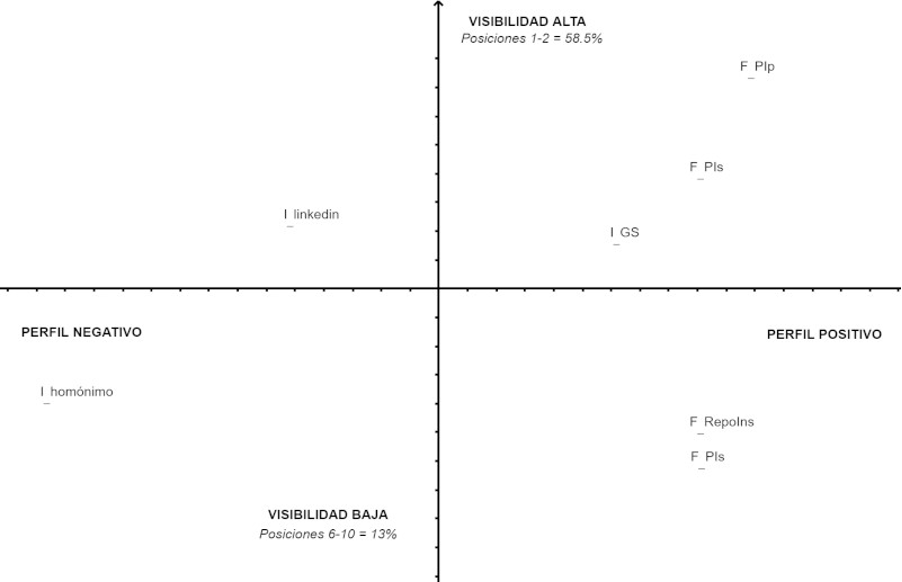
\includegraphics[keepaspectratio]{assets/imagenes/cap2_img1.png}}

}

\caption{\label{fig-1}Representación espacial de los indicadores de
visibilidad y la tipología de los sitios web}

\end{figure}%

\begin{enumerate}
\def\labelenumi{\arabic{enumi}.}
\tightlist
\item
  \emph{Visibilidad Alta-Positiva}. Refiere a los sitios web que tienen
  mayor probabilidad de exposición (58.5\%) cuando las personas buscan
  el nombre propio del investigador desde el motor de búsqueda de
  Google. Estos sitios web fungen como la carta de presentación del
  investigador fuera del ámbito académico. La visibilidad es considerada
  positiva debido a que el perfil académico presenta una validación
  institucional, la cual transmite al mismo tiempo una carga simbólica
  de legitimación. Por ejemplo, no tienen el mismo peso en la percepción
  de las personas acceder al primer resultado de búsqueda y consultar el
  perfil del investigador en la página web del instituto donde éste
  labura que acceder a la información personal del investigador desde su
  página personal en Facebook e incluso desde Researchgate o
  Academia.edu. Los resultados de búsqueda que engloban a esta categoría
  sumaron el 29.3\% de los casos y corresponden, como ya se señaló
  antes, a las páginas institucionales donde los investigadores están
  adscriptos (categoría F\_PIp).
\item
  \emph{Visibilidad Alta-Negativa}. Corresponde a los sitios web que
  contienen el perfil de los investigadores con información incompleta o
  irrelevante desde el punto de vista académico y que por supuesto no
  está avalada por la institución. De ahí que se les haya asignado una
  connotación negativa. No obstante, por su posicionamiento en los
  primeros resultados de búsqueda estos sitios web presentan una alta
  exposición y probabilidad de consulta. En este rubro pudieron
  registrarse principalmente los casos de páginas de LinkedIn de los
  investigadores (I\_Linkedin) con el 8.7\% de casos. Además, se
  contaron con algunos registros de cuentas de Linkedin homónimas
  (I\_Lh), mismas que sumaron el 6.5\% de las ocurrencias. Este último
  caso puede sugerir que la falta de información sistemática sobre el
  perfil académico del investigador, alojada en páginas web con
  determinada reputación o seriedad, tiende a restar relevancia para el
  algoritmo de búsqueda, de ahí que la consulta con el nombre propio del
  investigador arroje resultados homónimos. De igual manera, la
  singularidad o popularidad de los apellidos (por ejemplo, un Hernández
  López \emph{versus} un Cetto Kramis) puede considerarse como un factor
  de distinción al momento en que el algoritmo de búsqueda expone la
  relevancia de los resultados.
\item
  \emph{Visibilidad Baja-Positiva.} Esta categoría reúne a los sitios
  web con información relevante sobre el perfil de los investigadores y
  que está avalada por la institución. Sin embargo, éstas presentan una
  baja visibilidad debido a que el algoritmo de búsqueda les asigna
  alguna posición entre los lugares 6 y el 10. En este grupo cabe contar
  a las páginas institucionales donde los investigadores colaboran sin
  contar necesariamente con la titularidad o adscripción definitiva, de
  ahí que se consideren páginas web formales pero secundarias (F\_PIs).
  Este rubro suma el 11.6\% de los sitios web. Además de estas
  instituciones formales, esta categoría registró a determinados
  repositorios institucionales donde se difunden parte de los resultados
  de investigación de los académicos (F\_RepoInst). Estos repositorios
  formales fueron lanzados con la intención de almacenar, organizar y
  difundir las publicaciones de los investigadores. Paradójicamente
  presentan una baja probabilidad de acceso al realizar una consulta de
  búsqueda por nombre del investigador. En conjunto, los registros que
  apuntan a este tipo de espacios web suman el 5.3\% de los casos
  observados.
\item
  \emph{Visibilidad Baja-Negativa.} Aquí cabe mencionar a los sitios y
  plataformas digitales que van a tener una probabilidad muy baja de
  visitas y que además no aportan valor de contenido sobre el perfil
  académico de los investigadores. No obstante, vale la pena señalarlos
  debido a que una considerable proporción (8.9\%) hace referencia a
  identidades homónimas. Como ya se ha señalado antes, este dato puede
  sugerir una falta de información relevante sobre el perfil público de
  los investigadores. De ahí que el algoritmo de búsqueda muestra
  identidades similares a las solicitadas en las consultas de búsqueda.
\end{enumerate}

\section*{Conclusiones}\label{conclusiones}

\markright{Conclusiones}

El tipo de información y la relevancia de los resultados de búsqueda han
permitido constatar hasta qué punto el perfil digital de los
investigadores guarda una correspondencia con sus características
propiamente académicas. Asimismo, esta propuesta metodológica ha ayudado
a evidenciar la influencia que tiene la información que nutre a las
plataformas digitales en la construcción de una suerte de
\emph{identidad digital,} la cual puede sumar validez o restar valor
simbólico según el tipo de plataforma digital (formal e informal) que
difunda el perfil académico.

Dependiendo del grado de relevancia que estimen los algoritmos de
búsqueda, la huella digital de las personas puede estar visible u oculta
en distintos grados. La relevancia de los resultados de búsqueda no
necesariamente expone a los sitios web en términos de objetividad,
veracidad y exhaustividad de sus contenidos. En ocasiones la posición de
los resultados de búsqueda suele reflejar las tendencias de búsqueda que
surgen al momento de realizar las consultas, resultados de orden
sincrónico que pueden influir subjetivamente sobre un tema en particular
e incluso en la reputación de una persona. Por ejemplo, durante esta
observación pudieron ubicarse un par de casos polémicos que ameritan
mención y que ponen de relieve el papel de los algoritmos de búsqueda en
visibilizar u ocultar determinado tema (ver Anexo).

Finalmente, este ejercicio de observación permitió constatar que una
apropiada difusión de la identidad en internet puede contribuir a formar
en los académicos un \emph{capital de visibilidad,} es decir, una serie
de referencias positivas sobre el perfil de los académicos que presenta
una alta probabilidad de acceso. Estas referencias no solo comunican el
perfil curricular del académico, también conducen al acceso a las
publicaciones y a generar potencialmente otro tipo de interacciones
dentro y más allá del mundo académico y las universidades. En este
sentido, las instituciones académicas y científicas, al igual que los
investigadores, deben de poner atención en la apropiada construcción de
perfiles académicos en las plataformas digitales, de lo contrario los
algoritmos se encargarán de realizar dicha labor con base en sus propios
criterios.

\section*{Anexo}\label{anexo}

\markright{Anexo}

Al escribir el nombre de un académico sobre la caja de búsqueda, Google
arroja resultados de autocompletado, una predicción de lo que
probablemente el usuario quiere encontrar sobre este particular término
(Figura~\ref{fig-2}). El autocompletado muestra las tendencias o
consultas recurrentes que han hecho los usuarios y que están
relacionadas con el término de búsqueda. Cabe recordar que los
resultados de búsqueda cambian constantemente ante la actualización
periódica del algoritmo y el constante incremento y cambio en el volumen
de información que éste analiza (Figura~\ref{fig-3}).

\begin{figure}

\centering{

\pandocbounded{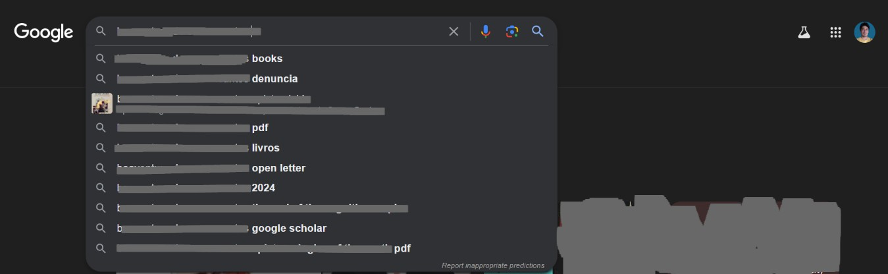
\includegraphics[keepaspectratio]{assets/imagenes/cap2_img2.png}}

}

\caption{\label{fig-2}Resultados de autocompletado para el nombre de un
académico (borrado por cuestiones de privacidad). En este ejemplo
destaca la palabra ``denuncia'', la cual lo involucra en un supuesto
tema de acoso.}

\end{figure}%

\begin{figure}

\centering{

\pandocbounded{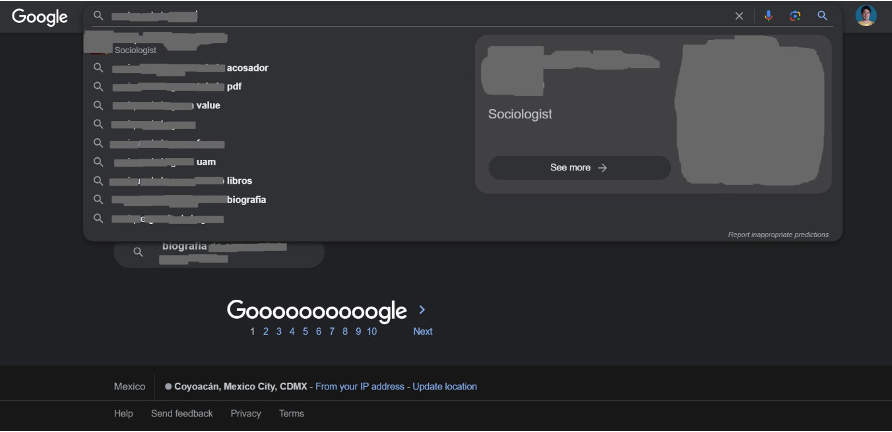
\includegraphics[keepaspectratio]{assets/imagenes/cap2_img3.png}}

}

\caption{\label{fig-3}Autocompletado de búsqueda que involucra a un
académico en un supuesto caso de acoso. Entre los primeros resultados se
muestra la palabra ``acosador''. En la actualidad (febrero de 2025) este
resultado de autocompletado ya no existe.}

\end{figure}%

\begingroup
\scriptsize

\begin{longtable}[]{@{}
  >{\raggedright\arraybackslash}p{(\linewidth - 4\tabcolsep) * \real{0.2917}}
  >{\raggedright\arraybackslash}p{(\linewidth - 4\tabcolsep) * \real{0.4861}}
  >{\raggedright\arraybackslash}p{(\linewidth - 4\tabcolsep) * \real{0.2083}}@{}}
\caption{Tipologías de sitios web. Ejemplo de las tipologías con mayor
frecuencia en la clasificación de los sitios web. Para fines de esta
propuesta solo se muestran los casos contrastantes que se mencionan en
el apartado de ``Tipología y grados de
visibilidad''.}\label{tbl-2}\tabularnewline
\toprule\noalign{}
\endfirsthead
\endhead
\bottomrule\noalign{}
\endlastfoot
& \begin{minipage}[t]{\linewidth}\raggedright
\begin{quote}
\textbf{FORMAL}
\end{quote}
\end{minipage} & \\
\begin{minipage}[t]{\linewidth}\raggedright
\begin{quote}
Página institucional primaria
\end{quote}
\end{minipage} & \begin{minipage}[t]{\linewidth}\raggedright
\begin{quote}
Sitio donde está adscripto el académico como investigador
\end{quote}
\end{minipage} & \begin{minipage}[t]{\linewidth}\raggedright
\begin{quote}
F\_PIp
\end{quote}
\end{minipage} \\
\begin{minipage}[t]{\linewidth}\raggedright
\begin{quote}
Página institucional secundaria
\end{quote}
\end{minipage} & \begin{minipage}[t]{\linewidth}\raggedright
\begin{quote}
Sitio donde está adscripto el académico como docente o realizando otras
funciones
\end{quote}
\end{minipage} & \begin{minipage}[t]{\linewidth}\raggedright
\begin{quote}
F\_PIs
\end{quote}
\end{minipage} \\
\begin{minipage}[t]{\linewidth}\raggedright
\begin{quote}
Repositorios Institucionales
\end{quote}
\end{minipage} & \begin{minipage}[t]{\linewidth}\raggedright
\begin{quote}
Repositorios o base de datos institucionales
\end{quote}
\end{minipage} & \begin{minipage}[t]{\linewidth}\raggedright
\begin{quote}
F\_RepoIns
\end{quote}
\end{minipage} \\
& & \\
& \begin{minipage}[t]{\linewidth}\raggedright
\begin{quote}
\textbf{INFORMAL}
\end{quote}
\end{minipage} & \\
\begin{minipage}[t]{\linewidth}\raggedright
\begin{quote}
Linkedin homónimo
\end{quote}
\end{minipage} & \begin{minipage}[t]{\linewidth}\raggedright
\begin{quote}
Nombre homónimo. No pertenece al investigador
\end{quote}
\end{minipage} & \begin{minipage}[t]{\linewidth}\raggedright
\begin{quote}
I\_Lh
\end{quote}
\end{minipage} \\
\begin{minipage}[t]{\linewidth}\raggedright
\begin{quote}
Linkedin
\end{quote}
\end{minipage} & \begin{minipage}[t]{\linewidth}\raggedright
\begin{quote}
Titular de la cuenta es el investigador
\end{quote}
\end{minipage} & \begin{minipage}[t]{\linewidth}\raggedright
\begin{quote}
I\_Linkedin
\end{quote}
\end{minipage} \\
\begin{minipage}[t]{\linewidth}\raggedright
\begin{quote}
Google Scholar
\end{quote}
\end{minipage} & \begin{minipage}[t]{\linewidth}\raggedright
\begin{quote}
Titular de la cuenta es el investigador
\end{quote}
\end{minipage} & \begin{minipage}[t]{\linewidth}\raggedright
\begin{quote}
I\_GS
\end{quote}
\end{minipage} \\
\begin{minipage}[t]{\linewidth}\raggedright
\begin{quote}
Sitios homónimos en general
\end{quote}
\end{minipage} & \begin{minipage}[t]{\linewidth}\raggedright
\begin{quote}
Sitio homónimo en general
\end{quote}
\end{minipage} & \begin{minipage}[t]{\linewidth}\raggedright
\begin{quote}
I\_homonimo
\end{quote}
\end{minipage} \\
\end{longtable}

\endgroup

\begingroup
\scriptsize

\begin{longtable}[]{@{}
  >{\raggedright\arraybackslash}p{(\linewidth - 10\tabcolsep) * \real{0.2566}}
  >{\raggedright\arraybackslash}p{(\linewidth - 10\tabcolsep) * \real{0.0973}}
  >{\raggedright\arraybackslash}p{(\linewidth - 10\tabcolsep) * \real{0.1239}}
  >{\raggedright\arraybackslash}p{(\linewidth - 10\tabcolsep) * \real{0.2566}}
  >{\raggedright\arraybackslash}p{(\linewidth - 10\tabcolsep) * \real{0.1062}}
  >{\raggedright\arraybackslash}p{(\linewidth - 10\tabcolsep) * \real{0.1239}}@{}}
\caption{Frecuencias (ƒ) de sitios web por tipo de
visibilidad}\label{tbl-3}\tabularnewline
\toprule\noalign{}
\endfirsthead
\endhead
\bottomrule\noalign{}
\endlastfoot
\begin{minipage}[t]{\linewidth}\raggedright
\begin{quote}
\textbf{Visibilidad} \textbf{Alta}
\end{quote}
\end{minipage} & & & \begin{minipage}[t]{\linewidth}\raggedright
\begin{quote}
\textbf{Visibilidad} \textbf{Baja}
\end{quote}
\end{minipage} & & \\
\begin{minipage}[t]{\linewidth}\raggedright
\begin{quote}
\emph{Categoría}
\end{quote}
\end{minipage} & \begin{minipage}[t]{\linewidth}\raggedright
\begin{quote}
ƒ
\end{quote}
\end{minipage} & \begin{minipage}[t]{\linewidth}\raggedright
\begin{quote}
\%
\end{quote}
\end{minipage} & \begin{minipage}[t]{\linewidth}\raggedright
\begin{quote}
\emph{Categoría}
\end{quote}
\end{minipage} & \begin{minipage}[t]{\linewidth}\raggedright
\begin{quote}
ƒ
\end{quote}
\end{minipage} & \begin{minipage}[t]{\linewidth}\raggedright
\begin{quote}
\%
\end{quote}
\end{minipage} \\
\begin{minipage}[t]{\linewidth}\raggedright
\begin{quote}
F\_PIp
\end{quote}
\end{minipage} & \begin{minipage}[t]{\linewidth}\raggedright
\begin{quote}
27
\end{quote}
\end{minipage} & \begin{minipage}[t]{\linewidth}\raggedright
\begin{quote}
29.3
\end{quote}
\end{minipage} & \begin{minipage}[t]{\linewidth}\raggedright
\begin{quote}
I\_
\end{quote}
\end{minipage} & \begin{minipage}[t]{\linewidth}\raggedright
\begin{quote}
41
\end{quote}
\end{minipage} & \begin{minipage}[t]{\linewidth}\raggedright
\begin{quote}
18.2
\end{quote}
\end{minipage} \\
\begin{minipage}[t]{\linewidth}\raggedright
\begin{quote}
F\_PIs
\end{quote}
\end{minipage} & \begin{minipage}[t]{\linewidth}\raggedright
\begin{quote}
9
\end{quote}
\end{minipage} & \begin{minipage}[t]{\linewidth}\raggedright
\begin{quote}
9.8
\end{quote}
\end{minipage} & \begin{minipage}[t]{\linewidth}\raggedright
\begin{quote}
F\_PIs
\end{quote}
\end{minipage} & \begin{minipage}[t]{\linewidth}\raggedright
\begin{quote}
26
\end{quote}
\end{minipage} & \begin{minipage}[t]{\linewidth}\raggedright
\begin{quote}
11.6
\end{quote}
\end{minipage} \\
\begin{minipage}[t]{\linewidth}\raggedright
\begin{quote}
I\_Linkedin
\end{quote}
\end{minipage} & \begin{minipage}[t]{\linewidth}\raggedright
\begin{quote}
8
\end{quote}
\end{minipage} & \begin{minipage}[t]{\linewidth}\raggedright
\begin{quote}
8.7
\end{quote}
\end{minipage} & \begin{minipage}[t]{\linewidth}\raggedright
\begin{quote}
I\_homonimo
\end{quote}
\end{minipage} & \begin{minipage}[t]{\linewidth}\raggedright
\begin{quote}
20
\end{quote}
\end{minipage} & \begin{minipage}[t]{\linewidth}\raggedright
\begin{quote}
8.9
\end{quote}
\end{minipage} \\
\begin{minipage}[t]{\linewidth}\raggedright
\begin{quote}
I\_
\end{quote}
\end{minipage} & \begin{minipage}[t]{\linewidth}\raggedright
\begin{quote}
7
\end{quote}
\end{minipage} & \begin{minipage}[t]{\linewidth}\raggedright
\begin{quote}
7.6
\end{quote}
\end{minipage} & \begin{minipage}[t]{\linewidth}\raggedright
\begin{quote}
I\_Gimages
\end{quote}
\end{minipage} & \begin{minipage}[t]{\linewidth}\raggedright
\begin{quote}
18
\end{quote}
\end{minipage} & \begin{minipage}[t]{\linewidth}\raggedright
\begin{quote}
8.0
\end{quote}
\end{minipage} \\
\begin{minipage}[t]{\linewidth}\raggedright
\begin{quote}
I\_Lh
\end{quote}
\end{minipage} & \begin{minipage}[t]{\linewidth}\raggedright
\begin{quote}
6
\end{quote}
\end{minipage} & \begin{minipage}[t]{\linewidth}\raggedright
\begin{quote}
6.5
\end{quote}
\end{minipage} & \begin{minipage}[t]{\linewidth}\raggedright
\begin{quote}
I\_docs
\end{quote}
\end{minipage} & \begin{minipage}[t]{\linewidth}\raggedright
\begin{quote}
14
\end{quote}
\end{minipage} & \begin{minipage}[t]{\linewidth}\raggedright
\begin{quote}
6.2
\end{quote}
\end{minipage} \\
\begin{minipage}[t]{\linewidth}\raggedright
\begin{quote}
I\_opinion
\end{quote}
\end{minipage} & \begin{minipage}[t]{\linewidth}\raggedright
\begin{quote}
6
\end{quote}
\end{minipage} & \begin{minipage}[t]{\linewidth}\raggedright
\begin{quote}
6.5
\end{quote}
\end{minipage} & \begin{minipage}[t]{\linewidth}\raggedright
\begin{quote}
F\_RepoIns
\end{quote}
\end{minipage} & \begin{minipage}[t]{\linewidth}\raggedright
\begin{quote}
12
\end{quote}
\end{minipage} & \begin{minipage}[t]{\linewidth}\raggedright
\begin{quote}
5.3
\end{quote}
\end{minipage} \\
\begin{minipage}[t]{\linewidth}\raggedright
\begin{quote}
F\_RepoIns
\end{quote}
\end{minipage} & \begin{minipage}[t]{\linewidth}\raggedright
\begin{quote}
5
\end{quote}
\end{minipage} & \begin{minipage}[t]{\linewidth}\raggedright
\begin{quote}
5.4
\end{quote}
\end{minipage} & \begin{minipage}[t]{\linewidth}\raggedright
\begin{quote}
I\_RG
\end{quote}
\end{minipage} & \begin{minipage}[t]{\linewidth}\raggedright
\begin{quote}
10
\end{quote}
\end{minipage} & \begin{minipage}[t]{\linewidth}\raggedright
\begin{quote}
4.4
\end{quote}
\end{minipage} \\
\begin{minipage}[t]{\linewidth}\raggedright
\begin{quote}
I\_GS
\end{quote}
\end{minipage} & \begin{minipage}[t]{\linewidth}\raggedright
\begin{quote}
5
\end{quote}
\end{minipage} & \begin{minipage}[t]{\linewidth}\raggedright
\begin{quote}
5.4
\end{quote}
\end{minipage} & \begin{minipage}[t]{\linewidth}\raggedright
\begin{quote}
F\_PIp
\end{quote}
\end{minipage} & \begin{minipage}[t]{\linewidth}\raggedright
\begin{quote}
8
\end{quote}
\end{minipage} & \begin{minipage}[t]{\linewidth}\raggedright
\begin{quote}
3.6
\end{quote}
\end{minipage} \\
\begin{minipage}[t]{\linewidth}\raggedright
\begin{quote}
I\_FBh
\end{quote}
\end{minipage} & \begin{minipage}[t]{\linewidth}\raggedright
\begin{quote}
4
\end{quote}
\end{minipage} & \begin{minipage}[t]{\linewidth}\raggedright
\begin{quote}
4.3
\end{quote}
\end{minipage} & \begin{minipage}[t]{\linewidth}\raggedright
\begin{quote}
SI\_
\end{quote}
\end{minipage} & \begin{minipage}[t]{\linewidth}\raggedright
\begin{quote}
7
\end{quote}
\end{minipage} & \begin{minipage}[t]{\linewidth}\raggedright
\begin{quote}
3.1
\end{quote}
\end{minipage} \\
\begin{minipage}[t]{\linewidth}\raggedright
\begin{quote}
I\_ACA
\end{quote}
\end{minipage} & \begin{minipage}[t]{\linewidth}\raggedright
\begin{quote}
3
\end{quote}
\end{minipage} & \begin{minipage}[t]{\linewidth}\raggedright
\begin{quote}
3.3
\end{quote}
\end{minipage} & \begin{minipage}[t]{\linewidth}\raggedright
\begin{quote}
I\_Gbooks
\end{quote}
\end{minipage} & \begin{minipage}[t]{\linewidth}\raggedright
\begin{quote}
6
\end{quote}
\end{minipage} & \begin{minipage}[t]{\linewidth}\raggedright
\begin{quote}
2.7
\end{quote}
\end{minipage} \\
\begin{minipage}[t]{\linewidth}\raggedright
\begin{quote}
I\_Gimages
\end{quote}
\end{minipage} & \begin{minipage}[t]{\linewidth}\raggedright
\begin{quote}
3
\end{quote}
\end{minipage} & \begin{minipage}[t]{\linewidth}\raggedright
\begin{quote}
3.3
\end{quote}
\end{minipage} & \begin{minipage}[t]{\linewidth}\raggedright
\begin{quote}
SI\_FBi
\end{quote}
\end{minipage} & \begin{minipage}[t]{\linewidth}\raggedright
\begin{quote}
6
\end{quote}
\end{minipage} & \begin{minipage}[t]{\linewidth}\raggedright
\begin{quote}
2.7
\end{quote}
\end{minipage} \\
\begin{minipage}[t]{\linewidth}\raggedright
\begin{quote}
\textbf{I\_homonimo}
\end{quote}
\end{minipage} & & & \begin{minipage}[t]{\linewidth}\raggedright
\begin{quote}
\textbf{F\_ArtIndex}
\end{quote}
\end{minipage} & & \\
& \begin{minipage}[t]{\linewidth}\raggedright
\begin{quote}
2
\end{quote}
\end{minipage} & \begin{minipage}[t]{\linewidth}\raggedright
\begin{quote}
2.2
\end{quote}
\end{minipage} & & \begin{minipage}[t]{\linewidth}\raggedright
\begin{quote}
5
\end{quote}
\end{minipage} & \begin{minipage}[t]{\linewidth}\raggedright
\begin{quote}
2.2
\end{quote}
\end{minipage} \\
\begin{minipage}[t]{\linewidth}\raggedright
\begin{quote}
I\_docs
\end{quote}
\end{minipage} & \begin{minipage}[t]{\linewidth}\raggedright
\begin{quote}
1
\end{quote}
\end{minipage} & \begin{minipage}[t]{\linewidth}\raggedright
\begin{quote}
1.1
\end{quote}
\end{minipage} & \begin{minipage}[t]{\linewidth}\raggedright
\begin{quote}
I\_NP
\end{quote}
\end{minipage} & \begin{minipage}[t]{\linewidth}\raggedright
\begin{quote}
5
\end{quote}
\end{minipage} & \begin{minipage}[t]{\linewidth}\raggedright
\begin{quote}
2.2
\end{quote}
\end{minipage} \\
\begin{minipage}[t]{\linewidth}\raggedright
\begin{quote}
I\_FBp
\end{quote}
\end{minipage} & \begin{minipage}[t]{\linewidth}\raggedright
\begin{quote}
1
\end{quote}
\end{minipage} & \begin{minipage}[t]{\linewidth}\raggedright
\begin{quote}
1.1
\end{quote}
\end{minipage} & \begin{minipage}[t]{\linewidth}\raggedright
\begin{quote}
I\_RGr
\end{quote}
\end{minipage} & \begin{minipage}[t]{\linewidth}\raggedright
\begin{quote}
5
\end{quote}
\end{minipage} & \begin{minipage}[t]{\linewidth}\raggedright
\begin{quote}
2.2
\end{quote}
\end{minipage} \\
\begin{minipage}[t]{\linewidth}\raggedright
\begin{quote}
I\_FBv
\end{quote}
\end{minipage} & \begin{minipage}[t]{\linewidth}\raggedright
\begin{quote}
1
\end{quote}
\end{minipage} & \begin{minipage}[t]{\linewidth}\raggedright
\begin{quote}
1.1
\end{quote}
\end{minipage} & \begin{minipage}[t]{\linewidth}\raggedright
\begin{quote}
F\_RepoN
\end{quote}
\end{minipage} & \begin{minipage}[t]{\linewidth}\raggedright
\begin{quote}
4
\end{quote}
\end{minipage} & \begin{minipage}[t]{\linewidth}\raggedright
\begin{quote}
1.8
\end{quote}
\end{minipage} \\
\begin{minipage}[t]{\linewidth}\raggedright
\begin{quote}
I\_Gmaps
\end{quote}
\end{minipage} & \begin{minipage}[t]{\linewidth}\raggedright
\begin{quote}
1
\end{quote}
\end{minipage} & \begin{minipage}[t]{\linewidth}\raggedright
\begin{quote}
1.1
\end{quote}
\end{minipage} & \begin{minipage}[t]{\linewidth}\raggedright
\begin{quote}
I\_SWps
\end{quote}
\end{minipage} & \begin{minipage}[t]{\linewidth}\raggedright
\begin{quote}
4
\end{quote}
\end{minipage} & \begin{minipage}[t]{\linewidth}\raggedright
\begin{quote}
1.8
\end{quote}
\end{minipage} \\
\begin{minipage}[t]{\linewidth}\raggedright
\begin{quote}
I\_RG
\end{quote}
\end{minipage} & \begin{minipage}[t]{\linewidth}\raggedright
\begin{quote}
1
\end{quote}
\end{minipage} & \begin{minipage}[t]{\linewidth}\raggedright
\begin{quote}
1.1
\end{quote}
\end{minipage} & \begin{minipage}[t]{\linewidth}\raggedright
\begin{quote}
I\_IGh
\end{quote}
\end{minipage} & \begin{minipage}[t]{\linewidth}\raggedright
\begin{quote}
3
\end{quote}
\end{minipage} & \begin{minipage}[t]{\linewidth}\raggedright
\begin{quote}
1.3
\end{quote}
\end{minipage} \\
\begin{minipage}[t]{\linewidth}\raggedright
\begin{quote}
I\_Wikipedia
\end{quote}
\end{minipage} & \begin{minipage}[t]{\linewidth}\raggedright
\begin{quote}
1
\end{quote}
\end{minipage} & \begin{minipage}[t]{\linewidth}\raggedright
\begin{quote}
1.1
\end{quote}
\end{minipage} & \begin{minipage}[t]{\linewidth}\raggedright
\begin{quote}
SI\_Gral
\end{quote}
\end{minipage} & \begin{minipage}[t]{\linewidth}\raggedright
\begin{quote}
3
\end{quote}
\end{minipage} & \begin{minipage}[t]{\linewidth}\raggedright
\begin{quote}
1.3
\end{quote}
\end{minipage} \\
\begin{minipage}[t]{\linewidth}\raggedright
\begin{quote}
SI\_
\end{quote}
\end{minipage} & \begin{minipage}[t]{\linewidth}\raggedright
\begin{quote}
1
\end{quote}
\end{minipage} & \begin{minipage}[t]{\linewidth}\raggedright
\begin{quote}
1.1
\end{quote}
\end{minipage} & \begin{minipage}[t]{\linewidth}\raggedright
\begin{quote}
SI\_TWi
\end{quote}
\end{minipage} & \begin{minipage}[t]{\linewidth}\raggedright
\begin{quote}
3
\end{quote}
\end{minipage} & \begin{minipage}[t]{\linewidth}\raggedright
\begin{quote}
1.3
\end{quote}
\end{minipage} \\
\begin{minipage}[t]{\linewidth}\raggedright
\begin{quote}
\textbf{Total}
\end{quote}
\end{minipage} & \begin{minipage}[t]{\linewidth}\raggedright
\begin{quote}
\textbf{92}
\end{quote}
\end{minipage} & \begin{minipage}[t]{\linewidth}\raggedright
\begin{quote}
\textbf{100.0}
\end{quote}
\end{minipage} & \begin{minipage}[t]{\linewidth}\raggedright
\begin{quote}
SI\_YouTi
\end{quote}
\end{minipage} & \begin{minipage}[t]{\linewidth}\raggedright
\begin{quote}
3
\end{quote}
\end{minipage} & \begin{minipage}[t]{\linewidth}\raggedright
\begin{quote}
1.3
\end{quote}
\end{minipage} \\
& & & \begin{minipage}[t]{\linewidth}\raggedright
\begin{quote}
I\_ACAr
\end{quote}
\end{minipage} & \begin{minipage}[t]{\linewidth}\raggedright
\begin{quote}
2
\end{quote}
\end{minipage} & \begin{minipage}[t]{\linewidth}\raggedright
\begin{quote}
.9
\end{quote}
\end{minipage} \\
& & & \begin{minipage}[t]{\linewidth}\raggedright
\begin{quote}
I\_FBr
\end{quote}
\end{minipage} & \begin{minipage}[t]{\linewidth}\raggedright
\begin{quote}
2
\end{quote}
\end{minipage} & \begin{minipage}[t]{\linewidth}\raggedright
\begin{quote}
.9
\end{quote}
\end{minipage} \\
& & & \begin{minipage}[t]{\linewidth}\raggedright
\begin{quote}
I\_Gral
\end{quote}
\end{minipage} & \begin{minipage}[t]{\linewidth}\raggedright
\begin{quote}
2
\end{quote}
\end{minipage} & \begin{minipage}[t]{\linewidth}\raggedright
\begin{quote}
.9
\end{quote}
\end{minipage} \\
& & & \begin{minipage}[t]{\linewidth}\raggedright
\begin{quote}
I\_GS
\end{quote}
\end{minipage} & \begin{minipage}[t]{\linewidth}\raggedright
\begin{quote}
2
\end{quote}
\end{minipage} & \begin{minipage}[t]{\linewidth}\raggedright
\begin{quote}
.9
\end{quote}
\end{minipage} \\
& & & \begin{minipage}[t]{\linewidth}\raggedright
\begin{quote}
I\_TWh
\end{quote}
\end{minipage} & \begin{minipage}[t]{\linewidth}\raggedright
\begin{quote}
2
\end{quote}
\end{minipage} & \begin{minipage}[t]{\linewidth}\raggedright
\begin{quote}
.9
\end{quote}
\end{minipage} \\
& & & \begin{minipage}[t]{\linewidth}\raggedright
\begin{quote}
varios
\end{quote}
\end{minipage} & \begin{minipage}[t]{\linewidth}\raggedright
\begin{quote}
12
\end{quote}
\end{minipage} & \begin{minipage}[t]{\linewidth}\raggedright
\begin{quote}
4.8
\end{quote}
\end{minipage} \\
& & & \begin{minipage}[t]{\linewidth}\raggedright
\begin{quote}
\textbf{Total}
\end{quote}
\end{minipage} & \begin{minipage}[t]{\linewidth}\raggedright
\begin{quote}
\textbf{225}
\end{quote}
\end{minipage} & \begin{minipage}[t]{\linewidth}\raggedright
\begin{quote}
\textbf{100.0}
\end{quote}
\end{minipage} \\
\end{longtable}

\endgroup

\nocite{Sued2022}
\printbibliography[heading=subbibliography, title={Referencias Bibliográficas}]

\chapter{Nuevas formas de narrar la realidad. El proceso de
individuación y su impacto en la escritura
académica}\label{nuevas-formas-de-narrar-la-realidad.-el-proceso-de-individuaciuxf3n-y-su-impacto-en-la-escritura-acaduxe9mica}

\addtocontents{toc}{\protect\hspace{1.5em}Paola Patricia Vázquez Almanza\par}
\markboth{Nuevas formas de narrar la realidad. El proceso de individuación y su impacto en la escritura académica}{}

\begin{flushright}
\Large Paola Patricia Vázquez Almanza\footnote{Facultad de Ciencias Políticas y Sociales, UNAM. Contacto: \href{paovaal@gmail.com}{paovaal@gmail.com}}

\end{flushright}

\section*{Introducción}\label{introducciuxf3n-1}

\markright{Introducción}

En la trilogía que compone \emph{La era de la información} (1999),
Manuel Castells ensayó una teoría sistémica que explica el impacto de
las nuevas tecnologías de la comunicación y la información. A lo largo
de esta obra, Castells planteó que la sociedad de fin de siglo se
transformaba en una red global de información y comunicación en la que
la generación, procesamiento y transmisión de información se convertiría
en una de las fuentes principales de producción y poder.

Aunque Castells anticipó que el siglo XXI traería nuevas desigualdades
derivadas del desarrollo tecnológico, jamás imaginó que en tan sólo unas
décadas transitaríamos de una era de la información a una era de la
desinformación. Si bien el autor previó que la transmisión de la
información sería un nuevo ámbito de poder, no sospechó que los poderes
político-económicos saturarían el espacio público con datos e
información falsa para causar desinformación y generar un ruido
comunicativo sin parangón.

No queda duda de que vivimos en una época marcada por las noticias
falsas, campañas de difamación, \emph{shitstorms}, propaganda electoral
y \emph{deep fakes}, adentrándonos en lo que se ha denominado
``posverdad''. El término ``posverdad'', según la RAE, es la
``distorsión deliberada que manipula creencias y emociones con el fin de
influir en la opinión pública'' (DRAE, 2014); y no es extraño que este
término haya sido seleccionado la palabra del año en 2016 por el
\emph{Oxford English Dictionary}, un año en el que los conservadurismos
y populismos comenzaron a expandirse con mayor fuerza alrededor del
mundo.

Aunque se puede argumentar que la información siempre ha sido una forma
de poder y que la manipulación de la opinión pública no es un fenómeno
nuevo, lo cierto es que la circulación rápida y expansiva de
información, facilitada por las redes sociales y los canales de
comunicación, hace que esta situación sea única y preocupante como se
comprobó durante la crisis sanitaria de la Covid-19.

Durante la pandemia, se generaron las condiciones idóneas para que las
prácticas de desinformación se volvieran cada vez más habituales y se
multiplicaron los retos provocados por los cambios sociales,
tecnológicos, ambientales, científicos y políticos del siglo XXI. Ante
esta crisis, numerosos investigadores y académicos de universidades
públicas se organizaron con el propósito de combatir las noticias falsas
y acercarse a la ciudadanía.

Estos esfuerzos fueron posibles gracias a que el clima de incertidumbre
mundial fomentó en la ciudadanía un deseo de encontrar fuentes
confiables de información para tomar decisiones y para comprender los
fenómenos estructurales que le afectan cotidiana y directamente. Y si
bien hubo un acercamiento entre academia y ciudadanía\footnote{A raíz de
  la pandemia de Covid-19, numerosas instituciones académicas en América
  Latina redoblaron esfuerzos para acercar la ciencia al público,
  priorizando una comunicación clara y pertinente desde sus centros de
  divulgación. Surgieron también colectivos de científicas y científicos
  dedicados a combatir la desinformación, como el grupo argentino
  ``Ciencia Anti Fake News'', creado por integrantes del CONICET para
  contrarrestar noticias falsas en tiempos de crisis sanitaria. De forma
  paralela, la UNAM, a través de su Programa Universitario de Estudios
  sobre la Democracia, Justicia y Sociedad, lanzó un curso especializado
  en la verificación y combate de noticias falsas. Estas acciones y
  debates sobre la importancia de la divulgación y la ciudadanización de
  la ciencia no se limitaron únicamente a la emergencia, sino que se
  mantienen vigentes en el entorno académico latinoamericano. Prueba de
  ello son los encuentros organizados posteriormente, como el evento
  ``aC-dC (antes del Covid-19 y después del Covid-19). Experiencias,
  aprendizajes y resignificaciones de la ciencia en pandemia'',
  convocado por la Academia Joven de Argentina, donde se discutieron
  estrategias de divulgación y experiencias de comunicación pública de
  las ciencias. Asimismo, en las Jornadas ``Escribir lo social'',
  especialistas en ciencias sociales, escritores y periodistas
  reflexionaron sobre diferentes formas de abordar y transmitir el
  conocimiento científico y social al público general.}, parece que esto
no fue suficiente para que las universidades públicas se replanteasen su
responsabilidad con la ciudadanía o su función social más allá de la
producción de conocimiento experto.

En su mayoría, las universidades siguen una tendencia hacia la
hiperespecialización, privatización del conocimiento, monetización de
los productos académicos, homogeneización de las formas de hacer
ciencia, refinamiento metodológico y una lógica neoliberal de producción
que ya desde finales del siglo XX preocupaba a autores como
Jean-François \textcite{Lyotard2019}, Russell \textcite{Jacoby2000},
Pierre Bourdieu (2009, 2011) y Zygmunt \textcite{Bauman1997}.

Estamos ante una transformación social que obliga a ampliar los alcances
del conocimiento científico a través del rediseño o actualización de las
categorías de análisis, de las formas de comunicar y de las
explicaciones producidas por las ciencias sociales. Es primordial
aprovechar esta oportunidad para realizar una autocrítica de las
ciencias sociales, poner a prueba la interdisciplinariedad y apoyar
institucionalmente los intentos de comunicar el trabajo científico de
manera más atractiva y relevante para un público no especializado.

Evidentemente esto no implica que todos los investigadores deban
necesariamente orientar sus hallazgos a la divulgación. Tan sólo se
quiere evidenciar la importancia que tiene actualmente legitimar y
fomentar la comunicación científica sobre lo social y seguir el ejemplo
de las denominadas ``ciencias duras'' en temas de la divulgación y
difusión de sus hallazgos. Asimismo, es importante aclarar que aunque la
divulgación de las ciencias sociales no constituye una etapa intrínseca
o indispensable de la labor científica, sí se relaciona con una función
social relevante del conocimiento generado en las universidades
públicas.

A la luz de los retos del presente, es imperativo que la academia no
sólo actualice sus métodos y objetivos, sino que también renueve su
forma de escribir y comunicar sus explicaciones de la realidad social. Y
con la finalidad de abrir este debate, este artículo abordará tres temas
principales: 1) la divulgación en el campo de las ciencias sociales, 2)
los efectos que tienen cambios sociales como el proceso de individuación
en la teoría social y 3) el doble rol de académicos y escritores que
asumen los cientistas sociales al hacer divulgación.

\section*{La divulgación más allá de la
forma}\label{la-divulgaciuxf3n-muxe1s-alluxe1-de-la-forma}

\markright{La divulgación más allá de la forma}

En las últimas décadas, las ciencias sociales se han acercado a otros
campos de conocimiento como la música o la biología, ganando así en
hibridez y obteniendo recursos para amplificar el entendimiento del
mundo social. Los coqueteos que autores clásicos de las ciencias
sociales como Durkheim, Weber o Marx tenían con la literatura o el arte,
el día de hoy se consolidan en las ``escrituras del yo'' y la
autoetnografía como en el caso de Didier Eribon, Alice Goffman, Ivan
Jablonka, Paulo Ravecca, Guy Bajoit o Lea Ypi. También se han dado
debates relevantes en torno a la escritura académica y a otras maneras
de narrar y comunicar los fenómenos sociales para un público general.

Una de las mayores apuestas de estos años ha sido apoyar la divulgación
de las ciencias sociales a través de medios no tradicionales para la
academia como podcast, textos híbridos y breves, fanzines, campañas en
redes sociales, bitácoras, videoblogs, \emph{tik toks}, memes o
infografías. Asimismo, se ha multiplicado notablemente la oferta de
diplomados, talleres y cursos de \emph{storytelling} dentro de las
instituciones universitarias para que los cientistas sociales aprendan a
hacer digerible y disfrutable el conocimiento que producen.

No obstante, la labor de divulgación de las ciencias sociales continúa
recibiendo poco apoyo institucional y se le dedica significativamente
menos análisis teórico y sistemático en comparación con otros procesos y
etapas de la investigación científica. De hecho, parece que tanto la
divulgación como la comunicación de los productos científicos siguen
considerándose algo alejado del quehacer científico. Por ello, no es
extraño que usualmente el esfuerzo de divulgar las ciencias sociales
fomente que los cientistas sociales asuman un doble rol: el de
académicos/investigadores y el de divulgadores/escritores

Y más allá de la doble vida que puede provocar el deseo de divulgar las
ciencias sociales, muchas veces no se cae en cuenta de que esos
ejercicios de divulgación se limitan a cambiar la forma en la que se
comunican estos académicos sin que esto implique una reflexión profunda
sobre cómo se está haciendo ciencias sociales actualmente y cómo
debiesen ajustarse a una realidad cambiante y cada vez más compleja.

Desde mi punto de vista, la divulgación de las ciencias sociales no
puede reducirse a lo estilístico o al medio, se requiere explorar
también su dimensión epistemológica, disciplinar y metodológica.
Replantear sólo el medio a través del que se comunica y refinar la forma
en la que se narra la realidad social puede aplazar, sin proponérselo,
la comprensión de las múltiples dimensiones que intervienen en la
búsqueda y puesta en práctica de formas alternativas de escribir y
comunicar las ciencias sociales.

Para comprender qué implica escribir y comunicar ciencias sociales,
habría que preguntarnos lo siguiente: ¿Qué tan necesaria es una
reflexión teórica y práctica sobre el proceso de escritura en las
ciencias sociales y sus dimensiones epistemológicas y metodológicas? Y a
partir de esta pregunta, habría que sumar otras tantas sobre cómo
actualizar las ciencias sociales que se hacen en las universidades
públicas y cómo crear audiencias que trasciendan el campus.

Nuevas realidades no sólo precisan otras formas de escribir y comunicar
las ciencias sociales, también requieren nuevas formas de interpretar la
realidad social. ¿Y cómo enfrentar este doble reto de renovar tanto las
formas de comunicar como las miradas a partir de las que las ciencias
interpretan y explican la sociedad?

Para responder estos cuestionamientos en los siguientes dos apartados
analizaré cómo los cambios sociales del siglo XXI afectan la teoría
social (en específico me interesa el proceso de individualización), y
cómo a partir de estas transformaciones sociales, se debe repensar y
actualizar la escritura académica, la divulgación de las ciencias
sociales, así como el punto de partida que se utiliza para comprender y
explicar la realidad social.

\section*{La doble vida: entre la academia y la
divulgación}\label{la-doble-vida-entre-la-academia-y-la-divulgaciuxf3n}

\markright{La doble vida: entre la academia y la divulgación}

En \emph{Para hablar de la sociedad la sociología no basta} (2019), el
sociólogo Howard Becker criticó la grisura y uniformidad de las
explicaciones proporcionadas por las ciencias sociales. En este libro,
el autor planteó que la mirada científica sólo alcanza a explicar una
fracción de la realidad por lo que las ciencias sociales están lejos de
monopolizar el conocimiento de ésta. Lo inabarcable de la realidad
empuja a los cientistas sociales a complementar las herramientas propias
de sus disciplinas con los recursos y puntos de partida que ofrecen
otros campos como el de la fotografía, el cine, el teatro o la novela.
Sólo recurriendo a otras formas de entender el mundo, escribe Becker, es
posible aminorar la brecha entre las explicaciones proporcionadas por
las ciencias sociales y la realidad.

Sin embargo, dicha brecha entre la realidad y las explicaciones
brindadas por las ciencias sociales no ha dejado de aumentar. Y por
ello, cada vez más la literatura sirve como una extensión analítica de
las ciencias sociales que ilumina aquello que desde la limitada mirada
científica no se logra percibir o narrar. Algunos cientistas sociales se
han percatado de la libertad narrativa que se puede obtener a través de
la literatura y han incorporado la autoetnografía y otros métodos, más
cercanos a la antropología que a la historia o a la sociología, para
analizar y narrar hechos sociales. Pareciera que los cientistas huyen de
sus disciplinas, de su rol de académicos, para escribir la realidad como
escritores, perpetuando así la doble vida que oscila entre ser
investigadores o divulgadores. Sólo los cientistas sociales más
consolidados han podido incorporar estos ejercicios de apertura
disciplinar a su carrera académica, como en el caso de Didier Eribon y
su obra \emph{Regreso a Reims} (2015) o Ivan Jablonka y su libro
\emph{La historia de los abuelos que no tuve} (2022).

Un ejemplo reciente que ilustra la existencia del doble rol de
académico/escritor es el caso de Lea Ypi y su novela \emph{Libre}
(2023). Lea Ypi, profesora de teoría política en la London School of
Economics y especialista en marxismo, decidió escribir una novela desde
la mirada personal para comprender el colapso del régimen comunista en
Albania a principios de la década de los noventa. Esta novela de
autoficción combina memorias, historia familiar, análisis político e
histórico con la finalidad de comprender los mecanismos de control del
régimen comunista y explicar el contexto en el que se dio la transición
a la democracia. La obra de Lea Ypi es tanto un recuento íntimo del
comunismo en Albania como una historia reciente del país balcánico. Pese
a que la novela de Ypi ha sido celebrada internacionalmente por dar
cuenta del régimen comunista albanés, su labor como cientista social y
su trabajo como escritora siguen estando totalmente disociados, como si
se tratase de dos formas completamente distintas de escribir, pensar e
interpretar la realidad.

Dicha disociación se relaciona en cierta medida con los prejuicios que
existen sobre el valor de la experiencia subjetiva del mundo y el género
de la literatura del yo o la autoficción. Y es que como señala el
escritor y politólogo César Tejeda en su libro \emph{La compulsión
autobiográfica} la escritura desde el yo se juzga como ``el medio
inapropiado para representar el mundo simbólicamente, como una moda,
como un producto del individualismo exacerbado de nuestros tiempos
{[}\ldots{]}, un acto de exhibicionismo'' \autocite[17]{Tejeda2022}.

Muchas de las críticas que Traverso plantea a lo largo de su libro son
acertadas y llaman a que los científicos sociales supervisen mejor sus
trabajos para que no pierdan rigor al ganar en estilo o subjetividad.
Sin embargo, me parece que Traverso no repara en la posibilidad de que
este fenómeno refleje, además de una democratización del ejercicio de la
escritura y de un repliegue neoliberal \autocite{Traverso2022} un
desplazamiento epistemológico. Es decir, quizás el vuelco hacia el yo es
síntoma también de una nueva forma de comprender el mundo que nos
obligaría a renovar las ciencias sociales, sus paradigmas, categorías y
formas tradicionales de analizar la sociedad, que sin duda también
podría llevar a una nueva manera de concebir la ecología de los saberes.

Danilo Martuccelli y José Santiago apuntan lo siguiente acerca de este
fenómeno:

\begin{quote}
El desarrollo contemporáneo del proceso de individualización obliga a
virar el rumbo de la sociología. Ante él no podemos seguir cerrando los
ojos y lamentar el lado oscuro que trae consigo: individualismo
exacerbado, egoísmo, privatización, competencia generalizada entre
actores. Ni explicarlo únicamente como el fruto de la gestión neoliberal
del capitalismo. Todo es ello es cierto, pero insuficiente. Nos
encontramos ante un proceso de mucho mayor alcance que desafía nuestro
modo de dar sentido y comprender lo social.
\autocite[209]{Martuccelli2017}.
\end{quote}

Si aceptamos el planteamiento de estos autores, podemos reconocer la
necesidad de redirigir la mirada de las ciencias sociales hacia los
sujetos para valorar sus experiencias de la realidad social y a partir
de ellas construir una interpretación actualizada de las sociedades
contemporáneas.

\section*{La experiencia individual al
centro}\label{la-experiencia-individual-al-centro}

\markright{La experiencia individual al centro}

Desde los primeros debates sobre la Modernidad\footnote{La sociología al
  ser heredera de la Modernidad ha arrastrado muchos de sus sesgos
  analíticos y puntos ciegos que han terminado por imponer una manera
  única y legítima de comprender el mundo, dejando de lado y ocultando
  otras formas de construir saberes y vínculos con el mundo
  \autocite{Dubet2010}. Es importante no dejar de señalar este sesgo
  heredado que sigue presente en las ciencias sociales.}, el
protagonismo del individuo dentro de la teoría social fue innegable y la
condena del individualismo exacerbado se convirtió en algo común. Sin
embargo, el centro de las explicaciones de la realidad social no fue
necesariamente el individuo por mucho que se le pensara como una de las
caras que componían la sociedad.

Y actualmente, pese a lo mucho que se ha transformado la vida social,
seguimos explicando o ajustando la realidad a antiguas categorías
analíticas y a formas específicas de entender la sociedad que no
engarzan con el presente. Las explicaciones que parten de las
estructuras y los grandes procesos no necesariamente se corresponden con
la experiencia subjetiva de esas mismas realidades. Y esto en gran
medida se debe al proceso de individualización y al hecho de que las
instituciones tradicionales de la sociedad ya no son los principales
puntos de orientación.

Hoy la realidad social se construye e interpreta a partir de la mirada
del sujeto y esto no es bueno ni malo, simplemente es. Y si la distancia
entre lo vivido y el lenguaje de los analistas no hace más que aumentar,
es necesario repensar el nexo entre el individuo y la sociedad como
propone Danilo Martuccelli (2007: 23).

Para subrayar la utilidad de actualizar los puntos de partida analíticos
de las ciencias sociales y repensar el nexo experiencia
individual-realidad social, retomaré las reflexiones que algunos
teóricos sociales han hecho en torno al proceso de individualización,
las formas de hacer ciencia y la necesidad creciente de poner el foco
sobre la experiencia individual para interpretar acertadamente nuestro
tiempo.

Comencemos con las reflexiones de Danilo Martuccelli sobre el proceso de
individualización en \emph{Gramáticas del individuo} (2007). En este
libro se retoma el concepto de individualización para plantear que la
experiencia individual ya no está estandarizada y que las instituciones,
clases y roles sociales ya no brindan las mismas pautas de orientación.
A medida que se ha complejizado la sociedad, la relación del sujeto con
su entorno se ha hecho más difusa, y, si cada vez hay menos estabilidad
institucional, es necesario volver la mirada al individuo para aclarar
el sentido de sus acciones y trayectoria
\autocite[24]{Martuccelli2007a}.~Por ello, el proceso de
individualización es una pieza clave para comprender el mundo actual.

El sociólogo Danilo Martuccelli continuó sus investigaciones sobre el
nexo individuo-sociedad y publicó, en coautoría con José Santiago, el
libro \emph{El desafío sociológico hoy: individuo y retos sociales}
(2017). En dicha obra se advierte lo siguiente:

\begin{quote}
A poco que prestemos atención al incremento espectacular de la
literatura de autoayuda veremos hasta qué punto existe una fuerte
demanda social que busca respuestas sobre la imbricación de las
experiencias individuales con la vida social, que, sin embargo, no es
atendida por la sociología. \autocite[7]{Martuccelli2017}.
\end{quote}

Frente al hecho de que los individuos no cesan de singularizarse y se
rebelan contra los casilleros sociológicos, los autores proponen la
construcción de una sociología que parta de las experiencias
individuales y dé cuenta de la sociedad a escala de los individuos
\autocite[8-9]{Martuccelli2017}. Esta propuesta busca criticar y
complementar la idea de sociedad presentada por las teorías del
conflicto, la integración, la funcionalista y la marxista. Y se acerca
en muchos sentidos al planteamiento teórico que el sociólogo François
Dubet hace en \emph{Sociología de la experiencia} (2010). En este texto,
Dubet se aleja de la sociología clásica y rechaza el planteamiento de
que sistema y actor son caras (una objetiva y otra subjetiva) de un
mismo conjunto (2010: 227) y propone en su lugar una ``sociología de la
experiencia''.

Dicha sociología de la experiencia consiste en definir la experiencia
individual como una combinación de las lógicas de acción que vinculan al
actor a cada una de las dimensiones de un sistema. Y la dinámica
producida por esta actividad es la que constituye la subjetividad del
actor y su reflexividad \autocite[96]{Dubet2010}. A partir de esta
definición de la experiencia como objeto sociológico, Dubet ha
estudiado, por ejemplo, los significados que tienen para los individuos
las desigualdades, la discriminación, el resentimiento social y otros
fenómenos sin dejar de lado cómo se entretejen dichas experiencias
individuales con los procesos estructurales.

En \emph{El nuevo régimen de las desigualdades solitarias. Qué hacer
cuando la injusticia se sufre como un problema individual} (2023), Dubet
pone a prueba una sensibilidad sociológica cercana a la propuesta por
Martuccelli y Santiago y concluye el libro con la siguiente afirmación:
``la sociología debería esforzarse por comprender cómo se articulan las
pruebas individuales y los desafíos colectivos, vinculando
obstinadamente los extremos de una cadena que parece estar rota: el
eslabón individualista y el eslabón holista'' (2023: 329).

Estas reflexiones teóricas de Martuccelli, Santiago y Dubet llevan a
preguntarnos: ¿qué lugar debe ocupar actualmente el individuo en las
ciencias sociales? Ante esta interrogante, se podría recurrir a lo
escrito por Guy Bajoit en \emph{El cambio social. Análisis sociológico
del cambio social y cultural en las sociedades contemporáneas}, obra en
la que el autor afirma que es imposible comprender y explicar las
sociedades actuales si no se coloca al individuo al centro de las
investigaciones (2008: 14).

En \emph{El cambio social}, Bajoit sostiene que ``son las relaciones
entre los individuos, que buscan construir y realizar su identidad
personal por sus intercambios, las que permiten comprender la vida
social'' (2008: 19); y sugiere, en consecuencia, reconstruir la
sociología alrededor de las capacidades del sujeto (2008: 278).

Hay que advertir que este repliegue hacia lo individual al que se
refiere Bajoit no implica que el individuo pierda sus dimensiones
sociales. Al contario, la experiencia individual jamás se agota en el
sujeto, siempre es social porque, como afirma Jean-Luc Nancy, la
singularidad es indisociable de la pluralidad (2006, p.~48). En todo
caso, la labor de las ciencias sociales consistiría en localizar hacia
dónde se ha desplazado el nexo entre el individuo y la sociedad, entre
la biografía y los procesos sociales.

Es llamativo el hecho de que estos autores no sólo coincidan en la
necesidad de virar hacia la experiencia individual para comprender la
realidad social contemporánea, sino que también consideren que las
ciencias sociales deben ponerse al servicio de los actores
\autocites[XI]{Bajoit2008}[165-168]{Martuccelli2017}.

\section*{Conclusiones}\label{conclusiones-1}

\markright{Conclusiones}

En este texto se han analizado los efectos del proceso individuación en
los presupuestos teóricos de las ciencias sociales y cómo, a partir de
estos efectos, se puede repensar y actualizar la escritura académica y
la divulgación científica. Estas reflexiones en torno a la
individuación, la teoría social, la divulgación y la escritura académica
pueden propiciar la creación de nuevas agendas de investigación que
convivan con otras ya consolidadas con el objetivo de dar una mejor
explicación e interpretación de los fenómenos sociales.

Por lo tanto, debatir las formas de hacer y escribir las ciencias
sociales aumenta las posibilidades de comunicar efectivamente los
hallazgos a nuevas audiencias, fomentar un debate público informado y
avanzar hacia una democratización del conocimiento científico. Dicha
democratización podría ofrecer a la ciudadanía algunas herramientas
indispensables para comprender mejor su entorno, decidir sobre sí y
conocer su margen de acción frente a lo que le afecta personalmente. En
este sentido, unas ciencias sociales situadas en el presente idealmente
nos acercarían a una sociedad en la que los individuos entiendan las
limitantes que ejercen las estructuras sociales sobre sus vidas,
reconociendo el marco de acción y organización que pueden ampliar y
modificar.

No se trata únicamente de que los cientistas sociales sean capaces de
escribir de manera más atractiva sus hallazgos, sino de que se abra la
posibilidad de buscar nuevos puntos de partida epistemológicos,
metodológicos, teóricos y escriturales para pensar, explicar y comunicar
lo social. La propuesta teórico-práctica que planteo aquí tiene el
propósito de enfrentar el reto doble de renovar tanto las formas de
comunicar las ciencias sociales como los puntos de partida teóricos
desde los que las ciencias sociales interpretan y explican la realidad.
Sólo al reflexionar en torno a las dimensiones epistemológicas,
metodológicas y teóricas del proceso de escritura dentro de las ciencias
sociales, será posible disminuir la brecha que existe actualmente entre
las explicaciones proporcionadas por estas disciplinas y la realidad
social.

\nocite{Castells1996, RealAcademiaEspanola2014, Bourdieu2009, Bourdieu2011, Becker2019b, Jablonka2022, Ypi2023, Dubet2023}
\printbibliography[heading=subbibliography, title={Referencias Bibliográficas}]

\chapter{Ensayo sobre un pódcast de investigación
sociológica}\label{ensayo-sobre-un-puxf3dcast-de-investigaciuxf3n-socioluxf3gica}

\addtocontents{toc}{\protect\hspace{1.5em}Fernando Rodrigo Beltrán Nieves\par}
\markboth{Podcast de Investigación Sociológica}{}

\begin{flushright}
\Large Fernando Rodrigo Beltrán Nieves\footnote{Universidad Autónoma Metropolitana, unidad Lerma. Contacto: \href{f.beltran@correo.uam.ler.mx}{f.beltran@correo.uam.ler.mx}}
\end{flushright}

\section*{Introducción}\label{introducciuxf3n-2}

\markright{Introducción}

El ecosistema del audio de nuestro tiempo ha venido participando con
gran intensidad en las reglas de producción e intercambios de bienes
culturales en la galaxia internet. Definen a este ecosistema el registro
de la voz o de las voces, la intervención del sonido y una posproducción
esmerada posterior. En este sentido el audio contemporáneo es un medio
de exigencia técnica como conceptual. Los intercambios entre la voz y el
sonido son múltiples y experimentales, rasgos característicos de la
expansión de este ecosistema particular. En dicho ecosistema convergen
además audiencias segmentadas. La escucha es ultra individual y se da
por medio de los auriculares. Además, la conexión al ecosistema es
posible gracias a los teléfonos personales inteligentes. Este ecosistema
particular es un medio vertiginoso, en permanente redefinición, de
amplio interés para las audiencias que nacieron en ambientes digitales y
rondan los veinte años. El ecosistema del audio ha expandido sus usos y
su influencia en una época de ``cansancio visual''
\autocite{Carrion2020} . Se afirma también que es una ``época de oro''
para los productores-creadores de sonido \autocite{Farra2020}. Estos
señalamientos y configuraciones recientes del ecosistema del audio han
posibilitado nuevas y no tan nuevas interrogantes de investigación en
materia de Ciencias Sociales. En este sentido elaboramos ahora preguntas
relativamente distintas con respecto al pasado más inmediato. Solemos
ahora cuestionarnos a qué suenan las cosas o los espacios que nos
gustan. Nos interrogamos también a qué suenan las Ciencias Sociales de
nuestro tiempo o cómo están interactuando los departamentos de
investigación académica con el ecosistema del audio.

Estas formulaciones muestran a un ecosistema del audio en mutación
constante. La conversación y, en menor medida la narración, circulan con
abundancia en el audio. No todo, sin embargo, puede desplegarse en el
medio. ¿Cómo funciona la reflexión teórica o la ensayística en el audio?
¿Qué clase de diseños de texto, de divulgación-difusión y diseños
sonoros logran potenciar el formato clásico de una investigación en
materia de Ciencias Sociales? ¿Cómo investigamos o escribimos para ser
escuchados? ¿Cuáles son las mejores condiciones o los mejores ambientes
---además de unos audífonos apropiados o una banda ancha de conexión---
para transmitir una investigación sociológica? Algunas respuestas
satisfactorias necesitan primeramente delinear con mayor precisión la
trayectoria general del ecosistema del audio.

\section*{Un ecosistema en
expansión}\label{un-ecosistema-en-expansiuxf3n}

\markright{Un ecosistema en expansión}

Un entramado de dispositivos tecnológicos y aplicaciones conectados a
internet que se actualizan con vértigo ha creado un sofisticado
ecosistema cultural global. En el pasado bastaba quizá un boletín
impreso, una revista periódica, la publicación de un libro, la
asistencia a una conferencia magistral para informarnos, comunicarnos,
estudiar o leer. En este ecosistema cultural global, por el contrario,
rige la híper-velocidad, los algoritmos creativos, la viralidad, la
ligereza, los contenidos híbridos y compactos, la inteligencia
artificial, la espectacularidad.

En su ensayo sobre la mutación cultural de nuestra época, Alessandro
Baricco ofrece una panorámica de esta ``lógica bárbara'' que domina el
ecosistema cultural global: ``la superficie en vez de la profundidad, la
velocidad en vez de la reflexión, las secuencias en vez del análisis, el
\emph{surf} en vez de la profundización, la comunicación en vez de la
expresión, el \emph{multitasking} en vez de la especialización, el
placer en vez del esfuerzo'' \autocite[epílogo]{Baricco2006}. En suma,
hablamos del ``\emph{storytelling}'' de la civilización digital. Además,
vivimos ahora una época multicanal. Una sensación de obligatoriedad de
estar en todos los canales, en todas las frecuencias, en todas las
plataformas. Las mensajerías instantáneas y las redes sociales, por lo
demás, son las autopistas que juzgamos indispensables para informarnos,
comunicarnos, entretenernos, estudiar y leer.

El audio, además, se ha configurado en una galaxia particular del más
vasto ecosistema cultural global. Dispositivos como iPhones, Siri, Apple
Podcasts, Alexa, WhatsApp, Spotify, Telegram, etcétera, protagonistas
visibles y poderosos del ecosistema del audio, han ido reconfigurando el
rostro y el ritmo de nuestros intercambios de bienes culturales. Las
innovaciones al interior del ecosistema del audio y, en innumerables
ocasiones, la sustitución del mensaje de texto por el mensaje de audio
en las mensajerías instantáneas incrustadas en los teléfonos
inteligentes personales, son aspectos indiscutibles del protagonismo de
esta galaxia particular.

En este sentido puede entenderse el impulso de la legendaria productora
radiofónica londinense, BBC, la cual está propugnando por sustituir la
noción de radio por el de audio y televisión por el de pantalla
\autocite{EspinosadelosMonteros2021}. Spotify es un caso global que
sintetiza la relevancia del audio dentro del ecosistema cultural global.
Entró al mercado estadounidense en 2014. Spotify instaló una innovación
que poco a poco logró estabilizar la escucha ultra individual de música
por medio de la suscripción, disponible a todo momento.

Empujado por la pandemia Covid-19, Spotify se concentró en 2020 en el
universo del pódcast, desplazando a la librería de audios hasta entonces
la más importante en el mundo anglosajón: Apple Podcast, antes iTunes.
Con Spotify en escena, circulan fuertes sumas de inversiones, contratos
espectaculares, ofertas originales de contenido
\autocite{Leijonhufvud2021}. \emph{Caso 63} es el ejemplo paradigmático
en el idioma español \autocite{StudiosSpotify2020,BeltranNieves2024}.
Habremos tardado en verlo de la siguiente manera: Spotify es al pódcast
lo que Netflix es a las series de televisión. Esta apuesta es relevante
porque a diferencia de la música, repetitiva y convencional, el pódcast
presume supuestos contenidos originales y o de calidad.

De la amplia gama de objetos culturales que se producen, navegan y se
consumen en nuestra actualidad, este ensayo se concentra en un fragmento
preciso: el diseño de audios listos para su descarga o escucha
ultra-individual. Este fragmento lo conocemos también como los pódcast,
que son archivos de audio en su expresión más simple, pero en el fondo
son diseños de textos, diseños de divulgación-difusión y diseños sonoros
en su forma. Los pódcast son diseños múltiples y han ido expandiendo sus
usos, sus posibilidades y sus fronteras. Interesa investigar con mayor
detenimiento la interacción de la investigación en materia de Ciencias
Sociales con el ecosistema del audio.

\section*{Objetos híbridos, diseños
múltiples}\label{objetos-huxedbridos-diseuxf1os-muxfaltiples}

\markright{Objetos híbridos, diseños múltiples}

Según el crítico catalán Jorge Carrión, el pódcast es un ``objeto
cultural vagamente identificado'' \autocite{Carrion2019}. OCVI en efecto
como un nuevo acrónimo en nuestra dieta cultural. Además de los pódcast,
según Carrión, nutren el especto de los OCVI los artefactos narrativos,
las listas de reproducción, los vídeos cortos, las obras negras, las
visualizaciones de análisis de datos, los \emph{tweets} e hilos de
\emph{tweets}. Esta clase de objetos buscan ser artísticos o
conceptuales, pero también divulgación-difusión. O a la inversa. Objetos
de divulgación-difusión que buscan ser artísticos o conceptuales.
``Objetos culturales vagamente identificados'' que circulan a grandes
velocidades por la galaxia internet.

El pódcast es un artefacto híbrido. Diseño, concepto y
divulgación-difusión son áreas mucho más fluidas en el ecosistema del
pódcast. Una escritura para ser escuchada, la pluralidad de las voces,
el sonido, los efectos del sonido, la gráfica y, ahora también, el uso
múltiple de la inteligencia artificial, cohabitan o se empalman en los
pódcast que surfean aerodinámicamente por las plataformas de audio y las
redes sociales.

Es indudable que el diseño, el concepto y la divulgación-difusión fueron
interconectados originalmente por la radio. Durante un siglo la radio
confirmó los usos múltiples de los guiones escritos, la voz o las voces
y los efectos de sonido. Radionovelas, experimentos radiofónicos,
radioteatro y apertura del medio a los creadores de vanguardia
\autocite[18]{Barea2002} fueron innovaciones que el nuevo medio en el
entonces avanzó con base sobre todo en las tradiciones literarias y
cinematográficas, configurándose muy rápidamente en una tradición
radiofónica propiamente dicha. Diseños provenientes de la radio que la
televisión más adelante heredó, se apropió y exploró ciertamente en sus
inicios, pero se estancaron con sus versiones comerciales posteriores,
repetitivas y convencionales.

Al reflexionar el nuevo medio durante la década de 1920, Bertolt Brecht
distinguió dos problemáticas distintas: \emph{1)} el uso del arte por
parte de la radio y \emph{2)} el uso de la radio por parte del arte
\autocite[8]{Brecht2003}. Dos intereses distintos que, según Brecht,
debían coindicir en una posibilidad compartida: la finalidad pedagógica.
En la época de expansión de la radio, Brecht enseguida le asestó una
dura crítica a la necesidad de saciar el hambre de contenidos. ``De
repente ---escribió Brecht--- se tuvo la posibilidad de decirlo todo a
todos, pero, bien mirado, no se tenía nada que decir''
\autocite[12]{Brecht2003}. Decir cualquier cosa a cualquiera es una
crítica brechtiana que pone en suspenso el generalizado recogocijo que
va de suyo con el crecimiento del ecosistema de los pódcast. Porque,
bien mirado, basta un micrófono y una cabina doméstica de grabaciones
para que cualquiera diga cualquier cosa, circule y se disperse en el
ecosistema. Ruido, barullo, conflicto de la interpretación circula
también, y en abundancia, en el ecosistema contemporáneo del audio.

En sus apuntes sobre la radio, además, Brecht rogaba inmediatamente por
el diseño de un medio que comunicara realmente. Una tecnología para que
el globo terráqueo encontrara intercambio entre todas las voces. Brecht
estaba inquieto por la escasa inversión en la radio pública berlinesa,
por la calidad de los contenidos, artísticos e inteligentes y, marxista
de suyo, por la difusión masiva de los contenidos. Y finalizaba algún
pasaje sobre la radio: ``Un hombre que tiene algo que decir y no
encuentra oyentes, está en una mala situación. Pero todavía están peor
los oyentes que no encuentran quien tenga algo que decirles''
\autocite[6]{Brecht2003}.

¿No es esta incógnita la que el ecosistema del pódcast ha creído
finalmente despejar?

Los traslapes en el ecosistema del audio acontecen con mayor naturalidad
en contraste con lo que ocurría en el pasado. La radio de ahora se
rediseña con los pódcast en escena, los pódcast mutan en programas de
radio o en diseños gráficos y las ficciones sonoras son adaptadas en
pantalla. Pablo \textcite{Fischer2021} distingue incluso entre
adaptaciones y traducciones en el intercambio, cada vez más
generalizado, entre las ficciones sonoras y las series de televisión.

El ecosistema del pódcast se ha afianzado, además, porque el audio es un
ambiente sonoro personalizado. Una personalidad afincada en tres
tradiciones distintas pero compatibles: no sólo la radiofónica, desde
luego, sino en una tradición literaria y otra cinematográfica
\autocite{EspinosadelosMonteros2020}. La radiofónica respalda el poder
de la voz o de las voces. La literaria confirma la fascinación por las
historias y la cinematográfica, entre otros aspectos, valida el
atractivo y la complejidad de los planos de la imagen o los ángulos del
sonido.

Este ecosistema ha impulsado la idea de que el medio garantiza el
derecho a hablar y a ser escuchado. Este ecosistema ha construido la
idea de que el pódcast es una expresión democrática: está en potencia al
alcance de los creadores y está disponible para los escuchas afines.
Este ecosistema sostiene que las relaciones entre los productores y los
usuarios son flexibles, son horizontales e interactivas. De tal suerte
que las relaciones son mucho más abiertas y participativas de lo que
ocurrió con la radio. La autoridad y las jerarquías no desaparecen,
desde luego, pero no se desenvuelven de forma vertical ni
unilateralmente. Es cierto que los requerimientos, las condiciones y el
conocimiento aplicado para lograrlo no se distribuyen de manera
universal. La ausencia de una conexión estable a internet o la de un
teléfono inteligente destruirían esta rebosante idea generalizada.

El pódcast en este sentido es ``tribal''
\autocite{EspinosadelosMonteros2021}, de unos pocos a más, de horizonte
potencial. Se estabiliza en comunidades que buscan contenidos
particulares que difícilmente la radio convencional, ya no digamos la
televisión tradicional, producen cotidianamente. En este sentido el
pódcast se asienta mucho más eficazmente en comunidades específicas:
libreros(as), escritoras(es), guionistas, artistas, bibliotecarios(as),
estudiantes, investigadores(as), departamentos universitarios. El
ecosistema del audio en suma conecta potencialmente con redes
específicas de individuos a través de sus teléfonos inteligentes
desperdigados en todo el globo.

Desde el punto de vista de los usuarios, la disponibilidad del
ecosistema del pódcast es la experiencia de escuchar
\emph{anytime}-\emph{anywhere} una emisión a la carta. Pero para los
productores o creadores, más importante aún, este ecosistema es una
respuesta a la necesidad de generar contenido específico, en flujo
constante, múltiple, diverso u original en el mejor de los casos, para
abrir otros canales de conversación, difusión-divulgación e intercambio.
Es una respuesta a la sentida necesidad de abrir canales específicos,
temáticos, porque sentimos las presiones de una ``época multicanal''.
Una expectativa o una posibilidad que la radio ha dejado en suspenso de
tiempo atrás porque en su práctica cotidiana ha optado por la
producción, gestión y difusión de contenido informativo, repetitivo y
convencional, apto para todos en teoría. El usuario del ecosistema del
pódcast, finalmente, puede adelantar o retroceder contenido, puede
ajustar la velocidad de reproducción o puede seleccionar también los
segmentos al interior del episodio por medio de las tablas de contenido.

\section*{Motivaciones de
apropiación}\label{motivaciones-de-apropiaciuxf3n}

\markright{Motivaciones de apropiación}

El pódcast como concepto o como diseño se encuentra en mutación
constante, en rediseño permanente. El pódcast se expande y tiene sed de
contenidos. La conversación, y en menor medida la narración, circulan
con abundancia en el audio. No todo sin embargo puede hacerse en el
medio. ¿Cómo podría funcionar la reflexión teórica o la ensayística en
el pódcast? Una adaptación fiel o inmediadta de un postulado teórico al
audio es posible, sin duda, pero estaríamos hablando formalmente de un
audiolibro. Frente a estas disyuntivas o imposibilidades, la emergencia
del pódcast académico ha sido una respuesta plausible del ecosistema. El
pódcast académico, difundido en inglés como ``\emph{scholar podcast}'',
ha dejado de ser una rareza de dicho ecosistema
\autocite{BeltranNieves2023}. En redefinición persistente, el pódcast
académico revive cuestiones sobre las tecnologías de la palabra, los
intercambios con la escritura, el diseño sonoro y el diseño de
``contenidos serios'' para escuchar. Con esta clase de innovaciones e
intercambios en circulación ha quedado en el pasado el ámbito de la
lectura aislada o arrinconada en las salas silenciosas de los recintos
universitarios y la escritura, por su parte, ha dejado de ser un
ejercicio solitario en algún lugar cómodo de la habitación. Nuestra
``humanidad aumentada'' \autocite{Baricco2019}, la extensión de todos
nuestros sentidos, se diversifica aún más con el ecosistema del audio en
expansión.

El pódcast académico problematiza el diseño apropiado para abrir nuevos
senderos y puertos para la investigación académica. Una preocupación por
el diseño que es también una discusión sobre el diseño sonoro. Hablamos
en suma de un diseño complejo para lograr un contacto afuera del
tradicional circuito de especialistas. O también, no menos importante,
para abrir otros canales de difusión e intercambio entre los
especialistas y públicos afines. Esto es así porque uno de los desafíos
más apremiantes del ecosistema cultural de nuestro tiempo es cómo
conectar con audiencias más amplias o audiencias más específicas o cómo
lograr una comunicación efectiva. Pero de igual modo cómo encarar los
retos de nuestro siglo: cómo interactuar artística y humanamente con la
inteligencia artificial.

El uso de técnicas narrativas por lo menos en la exposición de los
resultados de las investigaciones que se realizan es un modo recurrente
para lidiar con el ecosistema del audio. Son investigaciones que han
sido regularmente clasificadas como investigación de corte cualitativo o
a profundidad. Entre los géneros más habituales se encuentran
biografías, ensayos y relatos, entrevistas, testimonios e intervenciones
públicas. Esta propiedad textual, conceptualizada como ``narratividad''
\autocite{Lagmanovich2013}, favorece su traducción o adaptación
auditiva. Una posibilidad en términos de locución y sonoridad,
componentes fundamentales de la ``audicidad''
\autocite{BeltranNieves2022} de una escritura específica. Cuando
planteamos la relación entre la investigación en materia de Ciencias
Sociales y el audio nos referimos a esta traducción, intercambio o
adaptación de una escritura para ser escuchada. El concepto de
``audicidad'' \autocite[247-48]{BeltranNieves2022} refiere, por una
parte, a las dimensiones audibles y sonoras de un guion escrito, así
como a los montajes posteriores entre la escritura, la voz o las voces y
los planos del sonido. Por otra parte, este concepto refiere a los
encuentros posteriores entre el archivo de audio, las plataformas
digitales de audio y la apropiación de la escucha ultra individual por
medio de los auriculares personales.

Los intercambios habituales entre las investigaciones en materia de
Ciencias Sociales y el ecosistema del audio buscan una redirección
auditiva para diversos ejercicios o tentativas. Entre otros, sin orden
de importancia: \emph{1)} los de reflexión individual o colectiva;
\emph{2)} los de documentación de los hallazgos; \emph{3)} los de
crónica de los procesos simultáneos de toda investigación; \emph{4)} los
de licencia para disentir; y \emph{5)} los de las valoraciones de los
resultados \autocite[248]{BeltranNieves2022}. Sin embargo, ¿qué diseños
de texto, de divulgación-difusión y de sonido son adecuados para las
investigaciones que se realizan en materia de Ciencias Sociales? Desde
el punto de vista del diseño estricto, dos son los diseños
fundamentales: \emph{1)} el protagonismo de la voz o de las voces o
\emph{2)} la interacción de la voz o de las voces con el sonido en
distintos planos de intervención. El ``audio-artículo''
\autocite{UAMLerma2021} es un ejemplo del primer diseño y la ``ficción
académica sonora'' \autocite{FESAcatlan2022,FESAcatlan2023} lo es del
segundo. Entre ambas posibilidades existe de por medio un rango
experimental de matices. Finalmente, los diseños fundamentales, ya
advertidos, se alzan con base en guiones o soportes escritos, salvo los
pódcast llamados ``libres'', que prescinden del soporte textual. ¿Existe
en el horizonte otro modo de diseño y ejecución? Para ofrecer una
respuesta plausible a esta interrogante, quisiéramos detenernos en la
``técnica de interrupción''. Una figura sobre la que Maurice Blanchot,
Bertolt Brecht y Ricardo Piglia han reflexionado y usufructuado, cada
autor a su manera, usos y diversas posibilidades.

\section*{La interrupción}\label{la-interrupciuxf3n}

\markright{La interrupción}

Maurice Blanchot ha pensando la interrupción como figura teórica,
operador de lectura y categoría metodológica \autocite{Blanchot2008}. La
interrupción es una pausa que permite al habla convertirse en
conversación. La interrupción es una grieta o señal que posibilita la
interlocución, la continuidad (o no) del habla. Blanchot lo expresa de
este modo: ``la pausa que permite el intervalo; la espera que mide la
distancia infinita'' \autocite[98]{Blanchot2008}. En este sentido la
lengua auténtica, según Blanchot, es la lengua de la ``locura, el error
y la estupidez''. La interrupción es entonces una pausa, fisura,
intervalo, para introducir las diferencias, la ``diferencia infinita'',
la infinidad de posibilidades, la ``discontinuidad'', lo desconocido.
¿Qué clase de discontinuidades o diferencias? Digresiones, abismos,
repliegues, cumbres, vueltas. Con esta noción de interrupción, según
Blanchot, no puede darse la ``unidad de un discurso coherente''. La
narrativa o el hilo de lo que se cuenta, por su parte, puede ser
interrumpida en cualquier lugar. Existe en ella algo así como una
potencialidad latente de interrupción. No hay narración sin reflexión.
No hay narrativa sin dialéctica. La ironía, por ejemplo, según Blanchot,
descompone estos dos tropos habituales de la escritura literaria.

Otra clase de interrupción se da en la experiencia lectora. El lector se
interrumpe para desenmarañar (o no) el sentido de lo que lee. Un lector
ha leído durante un tiempo y entonces se detiene, se interrumpe, duerme.
La interrupción funciona aquí como una ruptura de la expectativa de
lectura. Hay otra clase de interrupción producida por la fatiga o el
cansancio. Una sentida necesidad de cortar de tajo las páginas que se
leen.

El escritor argentino Ricardo Piglia, por su parte, reflexionó en
algunos momentos sobre la interrupción como una técnica específica. Esta
técnica de intervención, según Piglia, fue apropiada por Bertolt Brecht
como un modo crítico de producción artística. En atención a Brecht,
según Piglia, la interrupción es una técnica o un instrumento de trabajo
para vincular dos inscripciones disímiles en un mismo lugar. Un modo de
``crear una realidad'' con base en dos registros disímiles pero
entretejidos, intercalados o yuxtapuestos. ``Discurso doble, poner un
texto dentro de otro, no por alusión, sino por doble inscripción de lo
escrito'' \autocite[294]{Piglia2015a}. En la técnica de interrupción son
fundamentales el corte narrativo y la yuxtaposición. Un modo de poner
los traslapes en escena, hacerlos visibles, propiamente audibles.

Si bien el ``teatro épico'' del dramaturgo alemán estuvo enmarcado de
modo general en el ``efecto de extrañamiento'' \autocite[§45,
47]{Brecht2019}, un efecto teorizado originalmente por el formalismo
ruso, la interrupción forma parte de los recursos de su ejecución.
Brecht lo buscaba afanosamente en múltiples niveles. ``Extrañamiento''
entre \emph{1)} el dramaturgo y la realidad social; \emph{2)} el plan
general de la obra y la escena-escena; \emph{3)} el actor y el
personaje; \emph{4)} lo musical, la mímica y la coreografía; \emph{5)}
el desempeño actoral, el público y la obra representada. En
consideración de los espectadores, el efecto lo buscaba Brecht al romper
la ilusión del escenario teatral a través de una ``escenografía no
realista'' o al poner en suspenso la identificación inmediata con los
personajes por medio del uso de máscaras o maquillaje exagerado para
resaltar su artificialidad. La interrupción en Brecht, además, operaba
con la incorporación de letreros, carteles o textos para avanzar algún
dato histórico en la representación o mediante estructuras narrativas no
cronológicas o no lineales o, asimismo, vía la introducción de coros
musicales en momentos exaltados de la obra. Un ``efecto de
extrañamiento'' para asestar una crítica a las problemáticas
político-sociales abordadas en el escenario. ``Para Brecht modificar los
procedimientos {[}dominantes{]} que regulan la producción artística
{[}v. gr. la mimesis, la ilusión o la identificación{]} es un modo de
intervenir específicamente ---a nivel del lenguaje y de los usos
sociales de la significación--- en la lucha de clases''
\autocite[68-69]{Piglia2015}.

Sobre variantes de la interrupción, finalmente, vale señalarse que, al
analizar espacios ``difíciles'' como la escuela, las habitacionales o
las urbanizaciones, Pierre \textcite{Bourdieu1999} pensó la
yuxtaposición de un modo similar a la de Brecht: es necesario el
abandono del punto de vista dominante, neutro o único. Espacios
``difíciles'' donde los individuos se encuentran ciertamente pero donde
todo los separa. Para inspeccionar estos espacios, según Bourdieu, es
insuficiente atender cada uno de los puntos de vista, sino que se trata
de ``poner de manifiesto, por el mero efecto de la yuxtaposición, lo que
resulta del enfrentamiento de visiones del mundo diferentes o
antagónicas'' (1999: 9). Estas yuxtaposiciones tienen su \emph{raison
d'être} en la estructura misma del mundo social.

En atención a lo expuesto aquí sobre las variaciones de la interrupción,
se trata ahora de definir un modo de intervenir \emph{1)} la narración,
\emph{2)} la reflexión conceptual y \emph{3)} lo ``discontinuo'' ---en
términos de Blanchot--- para los fines de un pódcast de investigación
sociológica. Narración, reflexión e inscripciones disímiles en un mismo
lugar constituirían un diseño híbrido, un diseño múltiple, un ``objeto
cultural vagamente identificado''.

\section*{Un pódcast de investigación
sociológica}\label{un-puxf3dcast-de-investigaciuxf3n-socioluxf3gica}

\markright{Un pódcast de investigación sociológica}

A diferencia de otros pódcast académicos donde la ``ficción sonora''
asume un rol protagónico (Fes Acatlán 2022, 2023), el diseño de un
pódcast de investigación sociológica que aquí se expone mantiene una
relación discreta con los planos de sonido. Los episodios de esta
iniciativa inspeccionan una serie de autores clásicos que contribuyeron
decisivamente al despegue de la Sociología. Marx, Engels, Durkheim,
Simmel, Weber, Parsons. Aunque sobre estos clásicos se ha escrito
indudablemente muchísimo, siguen formulándose interrogaciones sujetas a
la investigación de archivo o la investigación teórica. Son autores tan
fascinantes, además, que toda una agenda de investigación puede
plantearse en términos de rastrear minucias o huellas sobre las que la
crítica se ha detenido poco o pasa rápido sobre ellas. Son relatos
compactos que entretejen momentos biográficos con dimensiones del
contexto de producción de la obra teórica. Relatos breves, huellas,
marcas, microhistorias poco visitadas o desconocidas sobre los teóricos
que se juzgan decisivos. Para conectar aquí lo dicho sobre la técnica de
interrupción con el diseño de un pódcast de investigación sociológica es
conveniente mostrar una escaleta sencilla de un guion de locución. La
escaleta es un instrumento gráfico bastante extendido en las cabinas de
grabaciones. Si bien sus diseños son diversos, su utilidad reside en
reconocer el orden preciso de las voces: quién habla, qué se dice
exactamente, cuánto dura lo que se dice, así como precisar el orden de
intervención del sonido, pausas, transiciones o silencios.

\begingroup
\scriptsize

\begin{longtable}[]{@{}
  >{\raggedright\arraybackslash}p{(\linewidth - 8\tabcolsep) * \real{0.2180}}
  >{\raggedright\arraybackslash}p{(\linewidth - 8\tabcolsep) * \real{0.2180}}
  >{\raggedright\arraybackslash}p{(\linewidth - 8\tabcolsep) * \real{0.2180}}
  >{\raggedright\arraybackslash}p{(\linewidth - 8\tabcolsep) * \real{0.2180}}
  >{\raggedright\arraybackslash}p{(\linewidth - 8\tabcolsep) * \real{0.1053}}@{}}
\caption{Técnica de interrupción como diseño de locución. Elaboración
propia}\label{tbl-1}\tabularnewline
\toprule\noalign{}
\begin{minipage}[b]{\linewidth}\raggedright
Secuencia
\end{minipage} & \begin{minipage}[b]{\linewidth}\raggedright
Voz
\end{minipage} & \begin{minipage}[b]{\linewidth}\raggedright
Sonido
\end{minipage} & \begin{minipage}[b]{\linewidth}\raggedright
Contenido / Propósito
\end{minipage} & \begin{minipage}[b]{\linewidth}\raggedright
Duración
\end{minipage} \\
\midrule\noalign{}
\endfirsthead
\toprule\noalign{}
\begin{minipage}[b]{\linewidth}\raggedright
Secuencia
\end{minipage} & \begin{minipage}[b]{\linewidth}\raggedright
Voz
\end{minipage} & \begin{minipage}[b]{\linewidth}\raggedright
Sonido
\end{minipage} & \begin{minipage}[b]{\linewidth}\raggedright
Contenido / Propósito
\end{minipage} & \begin{minipage}[b]{\linewidth}\raggedright
Duración
\end{minipage} \\
\midrule\noalign{}
\endhead
\bottomrule\noalign{}
\endlastfoot
& & Introducción & Reconocimiento de apertura & 10'\,' \\
& Anfitrión(a) Disparador & & Presentación y objetivo del episodio & 30
a 45'\,' \\
& & Transición & Pausa & 5'\,' \\
Técnica de interrupción & Narrador(a) Analista & Voces y ambientación &
Conflicto & +10' \\
& Comentarista & Voces y ambientación & Clímax & +10' \\
& Aprendiz de sociólogo(a) & Voces y ambientación & Aceleración del
conflicto & +10' \\
& & Transición & Pausa & 5'\,' \\
& Anfitrión(a) & & Conclusión del episodio & 2' \\
& & Salida & Reconocimiento de salida & 10'\,' \\
& Créditos & Cortinilla institucional & & 1' \\
Total & & & & 15' \\
\end{longtable}

\endgroup

La Tabla~\ref{tbl-1} muestra una escaleta compuesta de 10 secuencias de
intervención. Las filas de la tabla identifican las secuencias y las
columnas distribuyen el contenido y los propósitos de dicho contenido:
las voces, quién dice qué, la duración medida según convenga en segundos
(doble comillas) o minutos (una comilla) y la intervención del sonido.
Las secuencias 01, 02, 03, 08, 09 y 10 son típicas entradas y salidas
generales de cualquier programa radiofónico o de cualquier pódcast del
ecosistema. Las secuencias 04, 05 y 06, en cambio, son los planos donde
la técnica de interrupción tiene lugar. Tipificadas como
``narrador(a)'', ``analista'', ``comentarista'' y ``aprendiz de
sociólogo(a)'', estas voces interactuan o se entretejen las veces que se
juzgan necesarias hasta agotar o abandonar el objeto de discusión.

Una historia que contar irrumpe como una vibración particular que
produce un ``campo magnético a su alrededor'' \autocite[4]{Baricco2023}.
Las historias que se cuentan, entonces, se estructuran regularmente
mediante la presentación de un conflicto, el clímax del conflicto y la
aceleración del conflicto o eventual resolución. Otras veces se edifican
mediante una noción rudimentaria de introducción, desarrollo y
conclusión de lo que se desea contar.

En este diseño propuesto la secuencia opera del siguiente modo: el
narrador comienza a narrar, pero es interrumpido por el analista quien
\emph{1)} matiza, acompaña o reflexiona al narrador o \emph{2)} trae a
cuento un registro teórico o variante: cita, aforismo, reflexión
conceptual. Y el analista, a su vez, o es interrumpido por el
comentarista quien dialoga con el analista o es cortado por el aprendiz
de sociólogo(a) quien introduce ``lo discontinuo'': una duda, una
\emph{boutade}, una reformulación innecesaria, un \emph{no sense}, una
afirmación apresurada o escandalosa, un extranjerismo. Es la
interrupción para volver a comenzar. El narrador retoma la narración y
la técnica de interrupción vuelve a operar. No se trata de un mecanismo
de intervención rígido o inmutable, sino flexible y adaptativo al
conflicto de lo que se cuenta o a la trayectoria del argumento central.
Este mecanismo, las secuencias 04, 05 y 06, funciona indefinidamente
hasta interrumpirse o concluir.

Vale resaltar el despliegue de la voz del ``aprendiz de sociólogo(a)'':
radicaliza la técnica de interrupción, introduce explícitamente ``lo
discontinuo'' en términos de Blanchot. Esta voz se nutre del
``\emph{storytelling}'' de la civilización digital: dispersa el sentido
``profundo de las cosas'', desritualiza lo sagrado, actúa con ligereza y
superficialidad, introduce el idioma inglés: en efecto, se trata del
``\emph{storytelling}'' de la civilización digital
\autocite{Baricco2006,Baricco2019}. En síntesis, esta voz singular es
una decisión fundamental en el diseño de un pódcast de investigación
sociológica. Es el plano sonoro para conectar dos mundos distintos: los
protagonistas fundamentales de la teoría sociológica y la cultura
digital. Un gesto pensado también para salir de los diseños habituales
del ecosistema del pódcast: o conversacionales o narrativos.

Interesa mostrar enseguida la puesta en práctica de la técnica de
interrupción como diseño ejecutable de un pódcast de investigación
sociológica. Un usuario conecta con una Inteligencia Artificial llamada
\emph{Milagros}, generadora de esbozos narrativos. La IA le sugiere al
usuario formular el prompt y enseguida sobreviene una narración que
atiende la inquietud. El usuario pide a la IA que incorpore en el relato
lo mucho o poco que sabe al respecto para sentirse cerca de la
discusión. Las voces que intervienen son las siguientes: Milagros IA de
esbozos narrativos, usuario, narrador, analista, comentarista y aprendiz
de sociólogo(a), que no es sino la transmutación del usuario en el
relato. Se trata de un esbozo referido al período berlinés de la vida
universitaria de Karl Marx\footnote{Para documentar dicho período
  {[}1835-1843{]} fueron consultados \textcite{Attali2019},
  \textcite{Duque1999}, \textcite{Dussel2008}, \textcite{Hegel2011},
  \textcite{Marx1987}, \textcite{McLellan1977}; Pérez Soto (2010, 2015,
  2019) y \textcite{Uroeva2017}.}.

\section*{Contrafactual sobre Karl
Marx}\label{contrafactual-sobre-karl-marx}

\markright{Contrafactual sobre Karl Marx}

\begin{transcripcion}
\item \escena{Sonido ambiente: se enciende una sofisticada interfaz digital y escuchamos un sonido positivo de bienvenida.}

\item \personaje{Milagros} Bienvenido, bienvenida, bienvenide, acabas de encender Milagros, una Inteligencia Artificial generadora de esbozos narrativos. Estoy diseñada para ayudarte en tus inquietudes formativas.

\item \personaje{Usuario} Mmm, hola, vaya. ¿Cómo funciona?

\item \personaje{Milagros} Formula el prompt y en instantes escucharás un relato justo a tu medida.

\item \personaje{Usuario} Bueno, Milagros, ¡yo soy marxista!

\item \personaje{Milagros} ¡Me alegro!, en estos días que corren ya no pululan los marxistas.

\item \personaje{Usuario} Bueno, mira, yo... yo no estoy tan seguro de qué pasaba cuando Marx entraba y salía de la Universidad de Berlín. Me gustaría descubrir algo sorprendente.

\item \personaje{Milagros} Te sugiero entonces formular: ¿qué hubiera pasado si la Universidad de Berlín hubiera incorporado a Marx en su plantilla docente? y en instantes te proporcionaré el relato que deseas escuchar.

\item \personaje{Usuario} ¿Un ejercicio contrafáctico sobre Karl Marx? Vaya, ¡me encanta!

\item \personaje{Milagros} Los ejercicios contrafactuales buscan despertar la curiosidad sobre las relaciones entre el pasado, nuestro presente y el futuro. ¿Qué hubiera pasado si...? es el punto de partida para plantear un ejercicio contrafactual.

\item \personaje{Usuario} Esta clase de esgrima intelectual no es habitual en las Ciencias Sociales.

\item \personaje{Milagros} Son ejercicios que siembran la duda sobre cómo se encadenaron los hechos que sucedieron. Redimensionan el peso de un componente, una pieza individual del amplio rompecabezas, para imputarle a la historia un cauce distinto a lo que ocurrió en verdad.

\item \personaje{Usuario} ¿Milagros?

\item \personaje{Milagros} ¿Deseas algo más?

\item \personaje{Usuario} Sí, bueno, me gustaría... ¿cómo decirlo? Me gustaría que yo aparezca también en el relato.

\item \personaje{Milagros} Generando una respuesta.

\item \escena{Sonido ambiente: sonido de transición a una dimensión desconocida.}

\item \personaje{Narrador} Cuando Karl Marx entraba y salía de la Universidad de Berlín, estaba sucediendo una de las batallas filosóficas más significativas de la primera mitad del siglo XIX.

\item \personaje{Analista} El saldo final de esta querella, adelantémoslo de una buena vez, fue la declarada bancarrota de Hegel, el filósofo cumbre de la época.

\item \personaje{Narrador} Muchos años después de esta polémica, en uno de sus prólogos a \textit{El Capital}, Marx recordaba cómo a Hegel se lo trataba todavía como "perro muerto". Corría el año de 1873 y el juicio lapidario pesaba todavía sobre la filosofía de Hegel.

\item \personaje{Analista} Por tal razón, en un arrebato de defensa o de indignación, Marx se declaró discípulo de Hegel. Esta afiliación de Marx redobla hasta nuestro presente el deseo de desterrar a Hegel o de ahogarlo en el silencio. O más habitual todavía: de criticarlo sin leerlo.

\item \personaje{Aprendiz de sociólogo / Usuario} \textit{I mean}, para el entendimiento de los mortales... los contemporáneos envidiosos de Hegel lo declararon muerto y, de paso, a todos sus \textit{mega fans}, Marx incluido. \textit{Is that right}?

\item \personaje{Narrador} Al poco tiempo de la muerte del profesor Hegel sobrevinieron las del ministro de Cultura y la del Rey absoluto de Prusia. Entonces el nuevo ministro de Federico Guillermo IV encendió las alarmas con la efervescencia de las interpretaciones radicales sobre Hegel de toda una nueva generación.

\item \personaje{Analista} Muerto Hegel el 14 de noviembre de 1831, subió de tono la disputa por su interpretación. Entre quienes resaltaban la filosofía de Hegel como una teología sofisticada y quienes la leían, en cambio, para criticarla o radicalizar sus razonamientos más sorprendentes u oscuros. No sólo era una encarnizada lucha de ideas filosóficas, sino un enfrentamiento entre generaciones. Una lucha por la definición material de la filosofía por medio del acceso a las cátedras universitarias o de su control.

\item \personaje{Aprendiz de sociólogo / Usuario} Me pregunto qué hubiera dicho el profesor Hegel sobre esta declarada bancarrota del filósofo Hegel.

\item \personaje{Analista} Se hubiera escabullido por el pasillo sin responder.

\item \personaje{Aprendiz de sociólogo / Usuario} \textit{Whyyyy}?!

\item \personaje{Analista} Porque... La filosofía llega siempre tarde. Cuando la filosofía pinta con sus tonos grises ya ha envejecido una figura de la vida que sus penumbras no pueden rejuvenecer, sino sólo conocer.

\item \personaje{Aprendiz de sociólogo / Usuario} ¿Y dicho menos filosóficamente?

\item \personaje{Analista} Los méritos de cada bando los hubiera visto con escepticismo o desconfianza. A cada bando, en todo caso, lo hubiera visto como un momento de lo verdadero en busca de algo más. Así como el búho de Minerva sólo emprende el vuelo al anochecer, Hegel hubiera preferido aguardar hasta la madurez de la disputa para conceptualizar, delinear y explicar.

\item \personaje{Narrador} El nuevo ministro en funciones convino entonces en la contratación del viejo filósofo Schelling para desterrar explícitamente la filosofía de Hegel y, sobre todo, a los hegelianos de la Universidad de Berlín. Antiguo amigo de Hegel, Schelling se tomó el tiempo de espera y programó su clase inaugural justamente en la conmemoración de la muerte de Hegel. Schelling expuso aquella vez una sentencia paradójica: la metafísica especulativa en boga (léase Hegel) es reaccionaria y subversiva. A esta clase inaugural asistieron Engels, Bakunin y Kierkegaard.

\item \personaje{Analista} Con Schelling en escena se instaló rápidamente un clima asfixiante para los jóvenes profesores hegelianos. Bauer, el asesor de tesis de Marx, devino exégeta de textos bíblicos. Feuerbach, de quien Marx tomó una imagen distorsionada sobre Hegel, se fue al campo a criar gallinas. Y Marx no tuvo ninguna opción en Berlín y se fugó para siempre de ahí.

\item \personaje{Aprendiz de sociólogo / Usuario} ¿Qué hubiera pasado si la Universidad de Berlín hubiera incorporado a Marx a su cuerpo docente?

\item \personaje{Analista} Sin duda se hubiese convertido en otro gran filósofo especulativo alemán, pero quizá no hubiera formulado uno de sus problemas filosóficos exquisitos de juventud.

\item \personaje{Aprendiz de sociólogo / Usuario} \textit{Which is}?

\item \personaje{Narrador} El problema de si al pensamiento humano se le puede atribuir una verdad objetiva.

\item \personaje{Analista} Este problema no es un problema teórico, sino un problema práctico. Porque es en la práctica donde el hombre tiene que demostrar la verdad, es decir, la realidad y el poderío, la terrenalidad de su pensamiento. El litigio sobre la realidad o irrealidad de un pensamiento que se aísla de la práctica es un problema puramente escolástico.

\item \personaje{Aprendiz de sociólogo / Usuario} Con bonito sabor a alguna tesis sobre Feuerbach.

\item \personaje{Narrador} ¿Qué hubiera pasado si la Universidad de Berlín hubiera incorporado a Marx a su cuerpo docente?, es una interrogante que pertenece al terreno de lo contrafactual.

\item \personaje{Aprendiz de sociólogo / Usuario} ¿Qué hubiera pasado? Fácil: ¡la Revolución Rusa no hubiera sucedido!

\item \personaje{Comentarista} \textit{Excuse me}?

\item \personaje{Analista} La Revolución Rusa necesitó de Marx, sin duda, pero necesitó igualmente de otras piezas significativas. Por ejemplo, que Engels, sin respiro, organizara, reescribiera y publicara durante los últimos 10 años de su vida, buena parte de los manuscritos, las notas de trabajo y borradores de Marx. O que los populistas rusos lectores de Marx, Lopatin y Danielson, tradujeran al ruso \textit{El Capital}.

\item \personaje{Narrador} Fue la primera traducción de \textit{El Capital} en aparecer y a circular en 1872.

\item \personaje{Analista} Marx es necesario para el estallido de la Revolución Rusa, diríamos, pero no suficiente.

\item \personaje{Narrador} Clausuradas las opciones en la Universidad de Berlín, Marx se doctoró en la Universidad de Bonn. Poco después, sin empleo y recién casado con Jenny von Westphalen, partió a Francia en 1843. Fueron los años donde murió una legítima aspiración, pero iniciaba con vértigo la pasión revolucionaria.

\item \personaje{Comentarista} Durante los primeros años de 1840, Marx se alejó para siempre de la carrera académica, pero escribió notables argumentos filosóficos. La mayoría de ellos no fueron publicados en vida de Marx. Entre los más célebres, las "Tesis sobre Feuerbach", \textit{La ideología alemana} o los \textit{Manuscritos económico-filosóficos} de 1844.

\item \escena{Sonido ambiente: sonido de transición de salida de una dimensión desconocida.}

\item \personaje{Milagros} Acabas de escuchar: \textit{Milagros IA: generadora IA de esbozos narrativos. Un pódcast de investigación sociológica}. Episodio uno: \textit{Contrafactual sobre Karl Marx}.

\item \escena{Sonido ambiente: sonido de desconexión.}
\end{transcripcion}

\section*{Conclusiones}\label{conclusiones-2}

\markright{Conclusiones}

El pódcast es un artefacto híbrido. Diseño, concepto y
divulgación-difusión son áreas mucho más fluidas en el ecosistema del
pódcast. Una escritura para ser escuchada, la pluralidad de las voces,
el sonido, los efectos del sonido, la gráfica y, ahora también, el uso
múltiple de la inteligencia artificial, cohabitan o se empalman en los
pódcast que surfean aerodinámicamente por las plataformas de audio y las
redes sociales.

Los pódcast en materia de Ciencias Sociales se han estado convirtiendo
en medios de producción, gestión y difusión de la investigación que se
realiza. En este sentido los pódcast de esta naturaleza problematizan el
diseño apropiado para abrir nuevos senderos y puertos para los objetos
de investigación. Una apuesta por el diseño que es también una discusión
simultánea por el diseño sonoro. Al igual que otros objetos culturales
de nuestra época, los pódcast académicos están definidos por rasgos que,
con la experimentación y la concurrencia, comienzan a estabilizarse en
distintos contextos o escenarios de la galaxia internet. Hablamos en
suma de un diseño complejo para lograr un potencial contacto afuera del
tradicional circuito de especialistas.

Sin embargo, los diseños fundamentales suelen ser narrativos o
conversacionales, siguiendo de cerca guiones o soportes escritos. Este
ensayo buscó justamente otro modo de ejecución y diseño. En efecto, en
atención a lo tratado en este ensayo sobre las variaciones de la
interrupción, se propuso la definición de un modo de intervenir
\emph{1)} la narración, \emph{2)} la reflexión conceptual y \emph{3)} lo
``discontinuo'' ---en términos de Blanchot--- para los fines de un
pódcast de investigación sociológica. Narración, reflexión e
inscripciones disímiles en un mismo lugar constituirían un diseño
híbrido, un diseño múltiple, un ``objeto cultural vagamente
identificado''. Un diseño apropiado para navegar aerodinámicamente por
la galaxia internet.

Finalmente, resaltamos el despliegue de la voz del ``aprendiz de
sociólogo(a)'' en el contrafáctico sobre Karl Marx, propuesto en este
ensayo. Esta voz materializa la técnica de interrupción, introduce ``lo
discontinuo'' en términos de Blanchot. Esta voz particular se nutre del
``\emph{storytelling}'' de la civilización digital: dispersa el sentido
``profundo de las cosas'', desritualiza lo sagrado, actúa con ligereza y
superficialidad, introduce el idioma inglés. Es justamente una
encarnación del ``\emph{storytelling}'' de la civilización digital. Es
una decisión fundamental en el diseño de un pódcast de investigación
sociológica. Es también el plano sonoro para conectar dos mundos
distintos: los protagonistas de la teoría sociológica clásica y la
cultura digital. Un gesto pensado para salir de los diseños habituales
del ecosistema del pódcast, conversacionales o narrativos.

\nocite{Perez2010, Perez2015, Perez2019}
\printbibliography[heading=subbibliography, title={Referencias Bibliográficas}]

\chapter{El pódcast como estrategia tecnopedagógica y transmedial en la
educación superior: el proyecto
Versatil}\label{el-puxf3dcast-como-estrategia-tecnopedaguxf3gica-y-transmedial-en-la-educaciuxf3n-superior-el-proyecto-versatil}

\addtocontents{toc}{\protect\hspace{1.5em}Diego Yael Valdez Serrano\par}
\markboth{El pódcast como estrategia tecnopedagógica y narrativa}{}

\begin{flushright}
\Large Diego Yael Valdez Serrano\footnote{Universidad Autónoma Metropolitana, unidad Lerma. Correo: \href{2193078912@correo.ler.uam.mx}{2193078912@correo.ler.uam.mx}}
\end{flushright}

\section*{Introducción}\label{introducciuxf3n-3}

\markright{Introducción}

La narrativa transmedia, entendida como la articulación de historias a
través de múltiples medios y plataformas, ha modificado de forma
sustancial la producción y el consumo de contenidos audiovisuales
\autocite{Scolari2013}. En este contexto, el pódcast ha ganado terreno
como un formato accesible y adaptable, capaz de ampliar los discursos
académicos y conectar con públicos diversos. Sin embargo esta expansión
no implica simplemente adaptar la misma historia a distintos formatos,
sino ofrecer contenidos únicos y complementarios en cada medio, con la
condición de que todos contribuyan al universo narrativo de forma
coherente e interconectada. \textcite{Scolari2013}, insiste en que ``no
son simplemente una adaptación de un lenguaje a otro\ldots{}'' sino una
auténtica red de significados ampliados, donde ``todos los medios
cuentan'' tanto desde el punto de vista de producción como de consumo.
Ese enfoque se articula con la noción de prosumidor propuesta por
Jenkins, donde parte de la audiencia no sólo recibe, sino que genera
contenido ---fanfiction, memes, análisis, etc.--- enriqueciendo la
experiencia transmedia \autocite{Jenkins2008}.

La tecnología no solo transforma nuestro entorno, sino que también
redefine la manera en que los sujetos interactúan con el conocimiento
\autocite{Scolari2013}. Hoy en día, el fácil acceso a dispositivos
digitales y a internet nos ha introducido en un ecosistema informativo
abundante, pero también caótico, donde la curaduría del contenido
adquiere un papel central.

La ``curaduría del contenido'', entendida como la selección estratégica
y crítica de la información en un ecosistema mediático saturado, tal
como plantea Scolari: es imprescindible ``una política de producción de
sentido'' que combine lenguajes diversos y plataformas
\autocite{MontoyaRojas2019}. El uso inteligente del pódcast permite
precisamente esa curaduría, posicionándose como un canal dinámico y
atractivo para ofrecer contenido especializado.

En este panorama, la adecuación de métodos y contenidos pedagógicos se
vuelve imperativa, especialmente ante una generación digital, inmersa en
múltiples pantallas desde sus primeros años. La sociedad digital ha
alterado profundamente nuestros modos de comunicación, aprendizaje y
participación ciudadana \autocite{Castells2006}, por lo que, resulta
urgente repensar los entornos educativos y sus estrategias de mediación.

La transformación digital, por su parte, impregna también las prácticas
educativas y comunicativas. \textcite{Castells2006}, describe la
sociedad contemporánea como una ``sociedad red'', caracterizada por
flujos de información constantes, virtualidad y conectividad. En este
contexto, la educación debe adaptarse a modelos pedagógicos que integren
estas dinámicas.

El pódcast, por su parte, no solo apoya la educación tradicional: ha
evolucionado hacia una \emph{metodología autónoma} de difusión
científica y cultural. Proyectos como ``My Gothic Dissertation'' de Anna
Williams demuestran cómo la producción de audio académico puede generar
comunidades de escucha activas y participantes \autocite{Williams2019};
y redes como Amplify Podcast Network en Canadá muestran el potencial del
pódcast institucional para legitimar nuevas voces académicas
\autocite{BeltranNieves2024}.

En el contexto mexicano, estas iniciativas aún se encuentran en fase
exploratoria, lo que representa una gran oportunidad para experimentar y
consolidar modelos propios. El caso del pódcast \emph{Versátil} se
analiza aquí como un experimento transmedia local de la Universidad
Autónoma Metropolitana unidad Lerma, que combina teoría, metodología y
narrativa: diez episodios que abordan temas de cultura y sociedad,
acompañados de publicaciones en redes y blog, conformando un
micro-universo narrativo. A través de entrevistas, recursos sonoros
originales y la participación de estudiantes y docentes, Versátil busca
consolidarse como ejemplo de ``educación sonora transmedia'' y
``alfabetismo mediático'' aplicado.

\section*{El pódcast como narrativa transmedia
emergente}\label{el-puxf3dcast-como-narrativa-transmedia-emergente}

\markright{El pódcast como narrativa transmedia emergente}

\textcite{Scolari2013} define la narrativa transmedia como una forma de
expandir una historia a través de múltiples plataformas, donde cada
medio aporta elementos únicos al conjunto. Esta lógica no busca repetir
lo mismo en distintos formatos, sino diseñar experiencias
complementarias que enriquezcan el universo narrativo. En este
entramado, el pódcast ocupa un lugar destacado como vehículo de
expansión, al permitir profundizar en aspectos específicos, brindar
nuevas perspectivas, o incluso ofrecer contenido original que no aparece
en otros soportes. Por ejemplo, un pódcast puede complementar una
película o serie mediante entrevistas, análisis, ficciones paralelas o
reflexiones críticas que nutran la experiencia narrativa.

\textcite{Jenkins2008}, uno de los pioneros en conceptualizar la
\emph{cultura de la convergencia}, subraya que las audiencias actuales
ya no son solo consumidoras pasivas, sino participantes activas en la
expansión del relato, a través de prácticas como el \emph{fanfiction},
la creación de memes, videos, análisis y pódcast. Esta cultura
participativa redefine las formas de producción, circulación y
apropiación del contenido, lo que convierte al pódcast en una
herramienta poderosa no solo de comunicación, sino de creación
comunitaria y significación colectiva.

Desde una perspectiva académica, esta expansión de contenidos se ha
transformado en una herramienta estratégica para la divulgación del
conocimiento. Esta tendencia responde, además, a una necesidad de
diversificar los lenguajes académicos y conectar con públicos más
amplios \autocite{Olivieri2022}. Actualmente es común encontrar en
plataformas digitales una amplia variedad de contenidos en audio: desde
entrevistas y conferencias hasta experimentos sonoros como ensayos en
audio, postales narrativas y diarios de campo sonoros. A esta gama
creciente, se suma ahora la producción de investigaciones sociales y
humanísticas diseñadas específicamente para el formato auditivo
\autocite{BeltranNieves2024}. No obstante, el entorno digital
contemporáneo se caracteriza por una sobreabundancia de información, un
fenómeno que \textcite{Levy1999} denominó ``infoproducción masiva'', y
por una atención cada vez más limitada por parte de los usuarios, algo
que \textcite{Franck2019} conceptualiza como la ``economía de la
atención''. En este contexto, el éxito de los contenidos digitales
depende de su capacidad para captar el interés en segundos. El pódcast
se enfrenta, por tanto, al reto de destacar en un ecosistema saturado.

Pese a ello, su valor reside en la capacidad de establecer vínculos más
personales con audiencias específicas. Gracias a su formato asincrónico,
flexible y su dimensión auditiva, los pódcast comienzan a ser parte de
una escucha activa y contextual, pues se escuchan mientras caminas,
cocinas, trabajas, estudias, manejas, etc, lo cual permitir una
experiencia distinta a la lectura o el video; generando una conexión
íntima con el oyente, el pódcast tiene una dimensión ``acústica y
afectiva'' que fortalece la comprensión, la reflexión crítica y el
compromiso emocional del oyente \autocite{Lindgren2016}. Este es
precisamente el punto de inflexión donde el lenguaje cobra una dimensión
auditiva y los creadores sonoros deben encontrar formas singulares y
creativas de narrar, persuadir y transmitir ideas.

Más allá de ser un canal de difusión, el pódcast puede convertirse en
una metodología de investigación. De acuerdo con
\textcite{McLoughlin2010}, el uso de herramientas digitales como el
pódcast promueve dinámicas colaborativas y reflexivas dentro de los
procesos investigativos cualitativos (Tabla~\ref{tbl-1}).

\begingroup
\scriptsize

\begin{longtable}[]{@{}
  >{\raggedright\arraybackslash}p{(\linewidth - 4\tabcolsep) * \real{0.3333}}
  >{\raggedright\arraybackslash}p{(\linewidth - 4\tabcolsep) * \real{0.3333}}
  >{\raggedright\arraybackslash}p{(\linewidth - 4\tabcolsep) * \real{0.3333}}@{}}
\caption{Beneficios de la producción de podcast. Elaboración propia a
partir de \textcite{McLoughlin2010}}\label{tbl-1}\tabularnewline
\toprule\noalign{}
\endfirsthead
\endhead
\bottomrule\noalign{}
\endlastfoot
\textbf{Categoría} & \textbf{Aspecto} & \textbf{Descripción} \\
Accesibilidad y bajo costo & Producción con recursos mínimos & Se
requiere poco equipo técnico y es fácil de distribuir digitalmente. \\
Estímulo al pensamiento crítico & Estructuración argumentativa & Obliga
a organizar la información de forma coherente y atractiva. \\
Interacción con la audiencia & Comunicación bidireccional & Permite
recibir retroalimentación y enriquecer el proceso pedagógico. \\
Expansión transmedia & Integración multimedia & Puede combinarse con
otros formatos como blogs, videos o redes sociales. \\
Flexibilidad de consumo & Adaptación al ritmo del oyente & Accesible
desde cualquier lugar y momento. \\
Mayor alcance & Audiencias más amplias & Puede superar barreras
geográficas y llegar a públicos diversos. \\
\end{longtable}

\endgroup

En este sentido, pensar el pódcast como narrativa transmedia emergente
implica reconocer su potencial para conectar lo académico con lo
cotidiano, lo teórico con lo afectivo, y lo digital con lo pedagógico.
Su desarrollo no debe limitarse al entretenimiento o la divulgación,
sino integrarse como práctica creativa, metodológica y crítica dentro
del quehacer investigativo y educativo. A pesar de sus múltiples
ventajas, la implementación del pódcast en contextos académicos y
educativos enfrenta diversos retos. Entre ellos destacan los obstáculos
técnicos (infraestructura, habilidades), pedagógicos (diseño didáctico,
evaluación) e institucionales (reconocimiento académico, tiempos de
producción) (Tabla~\ref{tbl-2}).

\begingroup
\scriptsize

\begin{longtable}[]{@{}
  >{\raggedright\arraybackslash}p{(\linewidth - 4\tabcolsep) * \real{0.3333}}
  >{\raggedright\arraybackslash}p{(\linewidth - 4\tabcolsep) * \real{0.3333}}
  >{\raggedright\arraybackslash}p{(\linewidth - 4\tabcolsep) * \real{0.3333}}@{}}
\caption{Dificultades de la producción de podcast. Elaboración propia a
partir de \textcite{McLoughlin2010}}\label{tbl-2}\tabularnewline
\toprule\noalign{}
\begin{minipage}[b]{\linewidth}\raggedright
\textbf{Categoría}
\end{minipage} & \begin{minipage}[b]{\linewidth}\raggedright
\textbf{Aspecto}
\end{minipage} & \begin{minipage}[b]{\linewidth}\raggedright
\textbf{Descripción}
\end{minipage} \\
\midrule\noalign{}
\endfirsthead
\toprule\noalign{}
\begin{minipage}[b]{\linewidth}\raggedright
\textbf{Categoría}
\end{minipage} & \begin{minipage}[b]{\linewidth}\raggedright
\textbf{Aspecto}
\end{minipage} & \begin{minipage}[b]{\linewidth}\raggedright
\textbf{Descripción}
\end{minipage} \\
\midrule\noalign{}
\endhead
\bottomrule\noalign{}
\endlastfoot
Barreras técnicas & Falta de competencias & La producción y edición
requieren formación específica. \\
Legitimidad académica & Escepticismo institucional & No siempre es
considerado un formato riguroso o válido para la investigación. \\
Tiempo de producción & Demanda de recursos temporales & Requiere
planificación, grabación, edición y difusión cuidadosa. \\
Curaduría de contenidos & Necesidad de actualización continua & Exige
mantener la información vigente y precisa. \\
Sostenibilidad & Financiamiento y permanencia & Es difícil mantener
proyectos sin modelos de apoyo económico o institucional. \\
\end{longtable}

\endgroup

La incorporación del pódcast como herramienta educativa dentro de un
enfoque transmedia representa una oportunidad significativa para
transformar las prácticas pedagógicas en la educación superior. Como lo
señalan \textcite{McLoughlin2010}, los entornos de aprendizaje mediados
por tecnologías digitales fomentan tanto la autonomía del estudiante
como procesos colaborativos más horizontales. En este sentido, los
beneficios del podcasting trascienden el simple uso del audio como
recurso didáctico: implican una reconfiguración de las dinámicas de
producción, circulación y apropiación del conocimiento.

Entre sus principales virtudes destaca su accesibilidad y bajo costo, ya
que permite la producción de contenidos con recursos mínimos y su
distribución digital es sencilla, lo que democratiza el acceso a la
información. Asimismo, el pódcast estimula el pensamiento crítico, al
exigir una estructuración argumentativa coherente y atractiva que
desafía tanto a quien produce como a quien escucha.

Desde una perspectiva transmedia, el pódcast adquiere un valor añadido
al poder integrarse con otros formatos como blogs, redes sociales o
videos, ampliando la experiencia educativa más allá de lo sonoro. Su
flexibilidad de consumo --accesible desde cualquier lugar y en cualquier
momento--, junto con su capacidad de alcance global, lo posicionan como
una herramienta ideal para entornos educativos híbridos,
descentralizados y adaptativos.

No obstante, es importante reconocer las dificultades que enfrenta la
producción de pódcast con fines educativos. En primer lugar, se
presentan barreras técnicas relacionadas con la falta de competencias en
producción y edición, lo que limita su adopción por parte del
profesorado. A ello se suma la cuestionada legitimidad académica del
formato, aún considerado por algunos sectores como insuficientemente
riguroso para la investigación científica. Además, el tiempo de
producción, la curaduría constante del contenido y la sostenibilidad
económica representan retos sustanciales, especialmente cuando no
existen apoyos institucionales o modelos claros de financiamiento.

En conclusión, el uso del pódcast educativo dentro de una estrategia
transmedia implica tanto potencialidades como tensiones. Su integración
efectiva en contextos universitarios requiere no solo de habilidades
técnicas, sino también de un cambio cultural que valore la diversidad de
formas en que se produce y se comparte el conocimiento. Como sostienen
\textcite{McLoughlin2010}, los entornos digitales no solo transforman
los medios, sino también los modos de aprender, enseñar e investigar.

\section*{Versátil: exploración de un pódcast universitario
emergente}\label{versuxe1til-exploraciuxf3n-de-un-puxf3dcast-universitario-emergente}

\markright{Versátil: exploración de un pódcast universitario emergente}

El pódcast \emph{Versátil}, se presenta como un espacio de difusión
cultural que refleja las inquietudes de la comunidad estudiantil a
través de una serie de ensayos narrativos en formato de audio, el cual
esta alojado en el canal de YouTube ATÓYATL, Difusión Cultural;
constituyendo una propuesta innovadora de comunicación universitaria que
integra contenidos culturales y académicos producidos por el
Departamento de Estudios Culturales de la Universidad Autónoma
Metropolitana (UAM), unidad Lerma.

En el marco de las narrativas transmedia y el uso tecnopedagógico del
pódcast en contextos educativos, su análisis permite identificar tanto
las potencialidades como las tensiones que surgen en su implementación.
El desarrollo formal del medio sonoro ha cobrado fuerza en la última
década. Los audios contemporáneos, disponibles en repositorios
digitales, bibliotecas en línea y plataformas de streaming, han
redefinido las formas en que nos relacionamos con la cultura. Como
señala \textcite{BeltranNieves2024}, esta evolución plantea nuevas
preguntas sobre los modos de producción y consumo simbólico en la era
digital.

\textbf{Accesibilidad, flexibilidad y alcance}. Una de las principales
fortalezas de \emph{Versátil} es su accesibilidad y bajo costo. Al
utilizar una plataforma abierta como YouTube, el pódcast puede ser
consultado sin barreras económicas o técnicas, respondiendo a uno de los
beneficios señalados por \textcite{McLoughlin2010}, quienes destacan que
las herramientas digitales pueden ser integradas a los entornos de
aprendizaje con relativa facilidad. Además, el formato asincrónico
incrementa la flexibilidad de consumo, permitiendo que los usuarios
escuchen los episodios en diferentes contextos, ritmos y dispositivos.
Esta disponibilidad también contribuye a su alcance global, superando
las limitaciones geográficas tradicionales.

\textbf{Estimulación del pensamiento crítico y diseño argumentativo}. En
los episodios de Versátil se observa una organización clara de los
contenidos, con narrativas estructuradas que abordan problemáticas
culturales y sociales desde una perspectiva crítica. El diseño de los
materiales en formato pódcast favorece el desarrollo del pensamiento
crítico, ya que exige a quienes participan en la producción planificar,
sintetizar y articular ideas de forma coherente y atractiva. La
participación de académicos como el Dr.~Fernando Beltrán Nieves, en la
coordinación general, y el Dr.~Juan Carlos López García del equipo
responsable de la producción, aporta un sustento discursivo sólido,
integrando referencias teóricas y fuentes relevantes dentro de la
narrativa de cada episodio.

\textbf{Interacción y dimensión transmedia}. El pódcast también se
beneficia del potencial interactivo que ofrece YouTube a través de los
comentarios, ``me gusta'' y suscripciones, mecanismos que pueden ser
utilizados para recoger retroalimentación y fomentar el diálogo con la
audiencia. Sin embargo, el desarrollo de una estrategia transmedia más
amplia permitiría enriquecer aún más la experiencia pedagógica.
Actualmente, \emph{Versátil} presenta una integración sistemática con
otros formatos como sitio web y redes sociales, sin embargo lo que
limita su expansión más allá del formato audiovisual, es su falta de
integración en otros medios como podría serlo, textos, publicaciones,
etc. La narrativa transmedia, como sugiere \textcite{Scolari2013},
requiere que cada medio aporte contenido específico y complementario,
algo que podría desarrollarse con mayor profundidad en futuras etapas
del proyecto.

\textbf{Limitaciones técnicas y de sostenibilidad}. Pese a sus méritos,
\emph{Versátil} enfrenta algunas barreras técnicas pues la falta de una
periodicidad clara sugiere que el pódcast puede estar limitado por
restricciones de tiempo y recursos humanos, coincidiendo con una de las
dificultades señaladas por \textcite{McLoughlin2010}: la producción de
contenidos digitales de calidad demanda planificación, habilidades
específicas y tiempo significativo. Por otra parte, la sostenibilidad
del proyecto es un aspecto crucial. No se observan mecanismos explícitos
de financiamiento, patrocinios o modelos de monetización, lo que podría
poner en riesgo la continuidad del pódcast a mediano y largo plazo. En
este sentido, sería recomendable explorar apoyos institucionales,
convocatorias culturales o alianzas estratégicas que respalden la
permanencia del proyecto.

\section*{\texorpdfstring{Análisis del episodio inaugural: ``\emph{La
sustancia}, una mirada crítica al cuerpo de la
mujer''}{Análisis del episodio inaugural: ``La sustancia, una mirada crítica al cuerpo de la mujer''}}\label{anuxe1lisis-del-episodio-inaugural-la-sustancia-una-mirada-cruxedtica-al-cuerpo-de-la-mujer}

\markright{Análisis del episodio inaugural: ``\emph{La sustancia}, una
mirada crítica al cuerpo de la mujer''}

El pódcast \emph{Versátil}, producido por el Departamento de Estudios
Culturales de la Universidad Autónoma Metropolitana, unidad Lerma,
representa una experiencia pionera en la convergencia entre narrativa
transmedia, crítica cultural y práctica tecnopedagógica. Su episodio
inaugural, titulado ``La Sustancia: una mirada crítica al cuerpo de la
mujer'', despliega una estrategia narrativa híbrida que conjuga ficción,
análisis social y ambientación sonora para abordar una de las
problemáticas más vigentes del ámbito mediático: la construcción y
consumo del cuerpo femenino.

\textbf{Narrativa y estructura crítica}: Desde su inicio, el episodio
utiliza la estructura de una película ficticia ---\emph{La Sustancia}---
como dispositivo argumental para interrogar los estándares estéticos
impuestos por la industria del entretenimiento. A través de la voz en
primera persona, diálogos dramatizados y ejemplos referenciales, se
construye un paralelismo entre la protagonista de la historia imaginaria
y figuras reales como Margot Robbie, Scarlett Johansson, Megan Fox,
Christina Aguilera y Donatella Versace. Esta estrategia narrativa no
solo aporta densidad argumentativa al discurso, sino que establece un
puente entre la ficción y la realidad cultural, elemento clave en las
narrativas transmedia \autocite{Scolari2013}.

El episodio está articulado mediante un guión sólido y progresivo, donde
cada elemento ---desde el planteamiento de preguntas críticas como
``¿Qué pasa si todas terminamos pareciéndonos entre nosotras?'' ---
hasta los silencios dramáticos--- está orientado a provocar reflexión y
participación emocional por parte del oyente. En línea con lo que señala
\autocite{Baricco2023}, la narración aquí no pretende ``decir la
verdad'' de forma literal, sino construir una experiencia significativa
a través de la exploración de esa verdad desde múltiples capas
simbólicas y sensoriales.

\textbf{Diseño sonoro y experiencia inmersiva}: Uno de los aciertos más
notables del episodio es su cuidado en la ambientación sonora: los
efectos ambientales, la música incidental y los momentos de silencio no
sólo acompañan el discurso, sino que potencian su significado. Este
recurso no es meramente estético, sino tecnopedagógico, en tanto
favorece la inmersión, estimula la atención del oyente y facilita la
internalización del contenido \autocite{McLoughlin2010}. El sonido, en
este caso, no solo enuncia, sino que construye atmósferas que provocan
sensaciones cognitivas y emocionales.

\textbf{Transmedia e intertextualidad cultural}: Aunque el episodio aún
no despliega una red transmedia expansiva (no se articula con blogs,
redes o plataformas adicionales), sí opera transmedialmente desde el
lenguaje narrativo y la intertextualidad. Al combinar ficción, análisis
y referencias culturales reconocibles, propone un discurso que puede ser
explorado desde múltiples lecturas. \textcite{Scolari2013} sostiene que
una narrativa transmedia se caracteriza por distribuir el contenido en
diversas plataformas, pero también por ofrecer capas narrativas que el
usuario puede descubrir y conectar, lo cual se cumple en este episodio
inaugural.

\textbf{Dimensión tecnopedagógica}: Desde una perspectiva educativa, el
episodio es un ejemplo de cómo el pódcast puede ser una herramienta
efectiva para el abordaje de contenidos complejos en contextos de
enseñanza superior. Al recurrir a formatos narrativos y sonoros no
tradicionales, promueve la reflexión crítica, el análisis de medios y la
comprensión de fenómenos sociales desde un lenguaje accesible pero
intelectualmente riguroso. Este enfoque responde a lo que
\textcite{McLoughlin2010} denominan \emph{aprendizaje participativo
digital}, donde el estudiante no solo recibe contenido, sino que lo
vive, lo interpreta y lo problematiza.

\section*{Conclusiones}\label{conclusiones-3}

\markright{Conclusiones}

El análisis del episodio inaugural (Tabla~\ref{tbl-3}) revela el
potencial del pódcast no solo como herramienta de divulgación, sino como
espacio de crítica cultural. El guión cuidadosamente estructurado, el
uso de referentes reales, la ambientación sonora y el enfoque narrativo
convierten a \emph{Versátil} en una apuesta innovadora para la creación
de contenidos educativos y reflexivos en la educación superior.

\begingroup
\scriptsize

\begin{longtable}[]{@{}
  >{\raggedright\arraybackslash}p{(\linewidth - 2\tabcolsep) * \real{0.5000}}
  >{\raggedright\arraybackslash}p{(\linewidth - 2\tabcolsep) * \real{0.5000}}@{}}
\caption{Análisis de Versátil. Elaboración
propia.}\label{tbl-3}\tabularnewline
\toprule\noalign{}
\endfirsthead
\endhead
\bottomrule\noalign{}
\endlastfoot
\textbf{Fortalezas} & \textbf{Oportunidades de mejora} \\
Estructura narrativa coherente & Refinar edición sonora y equilibrio de
audio \\
Calidad sonora adecuada & Fomentar llamada a la audiencia en el
episodio \\
Formato audiovisual accesible & Añadir referencias bibliográficas en la
descripción \\
Estímulo al pensamiento crítico & Integrar recursos transmedia (blogs,
redes, etc.) \\
Producción en plataforma gratuita & Aclarar periodicidad y
sostenibilidad \\
\end{longtable}

\endgroup

La propuesta del pódcast \emph{Versátil} demuestra que es posible
construir un discurso crítico y reflexivo utilizando herramientas
narrativas accesibles y formatos alternativos como el audio. A través de
una estructura cuidada y un enfoque temático relevante, el episodio
inaugural logra no solo analizar una obra cinematográfica, sino también
invitar al oyente a cuestionar las normas sociales que regulan la imagen
del cuerpo y el papel de la industria del espectáculo.

Uno de los principales aportes del proyecto reside en su capacidad para
activar el pensamiento crítico en los oyentes. El pódcast no solo
informa, sino que interpela, vincula y provoca una reflexión profunda
sobre los discursos culturales contemporáneos. La combinación de música,
efectos y entonaciones vocales contribuye a generar atmósferas que
refuerzan el contenido intelectual y emocional de cada episodio. A esto
se suma una narrativa ágil y versátil que evita la monotonía y mantiene
la atención de los oyentes.

Sin embargo, también es necesario reconocer las limitaciones
estructurales del formato. La producción de un pódcast educativo de
calidad exige habilidades técnicas específicas en grabación, edición y
diseño sonoro. En contextos universitarios donde estos recursos no están
disponibles, su implementación puede verse restringida.

Además, la credibilidad del pódcast dentro de los entornos académicos
tradicionales sigue siendo un reto. A pesar del creciente interés por
estos formatos, todavía persiste una discusión en su validación como
herramienta tecnopedagógica y su rigurosidad ante otros medios de
difusión científica. Esta percepción puede frenar su adopción
institucional. La inversión de tiempo también es un factor determinante.
El diseño de una narrativa transmedia coherente implica tareas que van
desde la planificación, una curaduría exigente, redacción de guiones,
postproducción y un profundo conocimiento de los públicos a los que se
dirige. Para muchos docentes e investigadores, este esfuerzo se suma a
una ya intensa carga laboral.

Otro desafío importante es la sostenibilidad. Sin un modelo claro de
financiamiento o apoyo institucional, la continuidad de estos proyectos
puede verse comprometida. La implementación de estrategias de
monetización o patrocinios, junto con políticas universitarias que
reconozcan el valor del pódcast como herramienta pedagógica, serían
pasos fundamentales para garantizar su permanencia.

El caso de \emph{Versátil} ilustra cómo el pódcast puede transformarse
en un medio poderoso para abordar temas sensibles, generar pensamiento
crítico y expandir los horizontes de la enseñanza universitaria. Su
narrativa transmedia, el uso creativo del sonido y su compromiso con la
reflexión cultural lo posicionan como un referente y una herramienta
valiosa para la educación contemporánea.

No obstante, su consolidación como práctica tecnopedagógica efectiva
dependerá de la capacidad de las instituciones educativas para reconocer
su valor, ofrecer formación técnica adecuada y facilitar su integración
en los planes de estudio. El pódcast no solo complementa el aprendizaje,
sino que lo reinventa, creando puentes entre el saber académico y la
cultura digital en la que los estudiantes están inmersos. Como señala
\textcite{Scolari2013}, cuando todos los medios cuentan, también debe
contarse con todos los medios. El reto está en hacerlo de forma crítica,
creativa y con vocación transformadora.

\printbibliography[heading=subbibliography, title={Referencias Bibliográficas}]

\part{ENTREVISTA}

\chapter{Eduardo Restrepo,
antropólogo}\label{eduardo-restrepo-antropuxf3logo}

\addtocontents{toc}{\protect\hspace{1.5em}Ignacio Moreno López\par}
\markboth{Entrevista a Eduardo Restrepo}{}

\begin{flushright}
\Large Ignacio Moreno López\footnote{Universidad Autónoma Metropolitana, unidad Lerma. Contacto: \href{i.lopez@correo.ler.uam.mx}{i.lopez@correo.ler.uam.mx}}
\end{flushright}

\begin{center}\rule{0.5\linewidth}{0.5pt}\end{center}

\begingroup
\footnotesize

Eduardo Restrepo es antropólogo colombiano egresado de la Universidad de
Antioquia (Medellín, 1996), con estudios de maestría y doctorado en la
University of Carolina del Norte en Chapel Hill. Dentro de sus líneas de
investigación se destacan los estudios referidos a las poblaciones
afrocolombianas, con particular interés en la región del Pacífico
colombiano. Los procesos de etnización y racialización, así como las
políticas de la representación y subjetividades políticas negras, son
algunos de los asuntos abordados en sus publicaciones. También se ha
interesado por las geopolíticas del conocimiento y los procesos de
lugarización que configuran campos disciplinarios como el de la
antropología o transdisciplinarios como el de los estudios culturales.

El objetivo de la entrevista es dar a conocer la diversidad de la
práctica científica a través de entrevistas abiertas que rescaten la
vida y devenir de personas relevantes de las ciencias sociales.
\endgroup

\begin{center}\rule{0.5\linewidth}{0.5pt}\end{center}

\begin{transcripcion}
\item \personaje{Ignacio} Muy buenas tardes a todas a todos y todes es bienvenidos a esta charla en la que hoy vamos a sentarnos con un colega y amigo Eduardo Restrepo. Quienes no tengan la suerte de conocer a Eduardo, que es una persona polifacética muy viajera y que ha hecho una de las grandes contribuciones a las rupturas y a los avances en determinados espacios, les voy a comentar que actualmente es un investigador adjunto del Centro de Investigación, Innovación y Creación de la Universidad Católica de Temuco y es profesor del doctorado de antropología de la misma universidad. Su formación es como antropólogo colombiano egresó hace ya unos añitos de hecho, creo que en breve van a ser 30 años si no me equivoco porque creo que egresaste en el 96 de la Universidad de Antioquia en Medellín. Para quienes no conozcan Colombia, es una de las principales ciudades del país y tuvo la oportunidad en su momento de realizar unos estudios de maestría y doctorado en la Universidad de Carolina del Norte en Chapel Hill. Además, fue presidente entre el 2015 y 2020 de la Asociación Latinoamericana de Antropología. Actualmente es profesor en diferentes universidades. Ya veréis a lo largo de la charla, que es una persona muy cercana a lo que llaman ciudadano del mundo en cuanto a su movilidad, en cuanto a su visión de la realidad y en cuanto a la apertura. Pues primeramente Eduardo agradecerte muchísimo esta entrevista que nos permitas entrar en tu vida y en tu mundo.

\item \personaje{Eduardo} Gracias a ti por la invitación y ya qué bueno que estemos conversando nuevamente.

\item \personaje{Ignacio} Sí, para quienes no sepan, ya tuvimos una entrevista que tristemente se perdió el audio, pero bueno eso nos da la excusa para volver un año después para volver a sentarnos a tomar un cafecito y a charlar un poco. Eduardo una cosa que interesa siempre a nuestro alumnado y a nuestros colegas obviamente nos interesa ¿quién es Eduardo hoy día? pero ¿quién fue Eduardo? ¿por qué Eduardo es quién es? porque en qué momento o qué recuerdos y de Medellín de tu infancia de esos primeros momentos que dijeron que fueron marcando un poco hacia dónde iría tu vida cuéntanos un poco cómo era la Medellín de los 80 qué tipo de vida, porque por desgracia pues ehh toda Colombia es consciente de los estereotipos no... de cómo tenemos predefinida por series de televisión y por literatura panfletaria la vida no, pero ¿cuál es la cotidianidad real o cuál es la cotidianidad que tú recuerdas de ese mundo?

\item \personaje{Eduardo} Yo nací en un barrio popular en Medellín que sigue mucho las características que estás mencionando: sí había bastante violencia. Crecí en uno de los barrios donde muchos de nosotros aspiramos a ser sicarios cuando teníamos 12 o 13 años de edad, donde Pablo Escobar era un referente de las armas, de muchas cosas... Pero también recuerdo mucho de haber crecido en la calle jugando con muchos amigos, jugando al fútbol, yendo a nadar. Para mí el recuerdo de la infancia de ese barrio popular es el un barrio muy lleno de cariño, de amistad, de mucha gente, de mucha música, de empatía, y a pesar de que era muy duro y muchos de quienes crecieron conmigo terminaron asesinados o terminaron en cruces o en la cárcel, de todas maneras, mi recuerdo es una experiencia muy cargada de historias muy llenas de afecto y también muy llenas de fuerza. Nuestros papás y mamás trabajaban en fábricas o trataban de rebuscarse la vida por diferentes lados. Yo fui la primera persona de mi familia que fue a la universidad a estudiar, algo como antropología donde me encontré con muchas conversaciones muy interesantes más allá de lo que se vivía en un barrio lleno de fútbol, de música salsa, de fierros y tropeles, pero también de mucha alegría y cariño.

\item \personaje{Ignacio} Era muy mexicano también.

\item \personaje{Eduardo} Es parecido a lo que ustedes están viviendo ahora.

\item \personaje{Ignacio} De hecho, una de las cosas que vemos en nuestra universidad es que tenemos la fortuna de muchos del alumnado que son la primera generación que llega a la universidad, ¿cómo vivió tu casa ese momento? en el que Eduardo dice no, pues yo voy a estudiar. O sea yo no voy a la fábrica, yo no voy a un taller, sino que voy a ir a la universidad, y además voy a estudiar una cosa y se llama antropología. No voy a estudiar ingeniería no voy a estudiar medicina no voy a estudiar derecho, no, ¿cómo fue esa situación? ¿recuerdas?

\item \personaje{Eduardo} Pues fue bastante curiosa. Recuerdo que uno de mis tíos, cuando supo que iba a la universidad, me recomendó que estudiara ingeniería química para que hiciera coca. Estudiar antropología obviamente era algo que no que no que cabía en el horizonte de sentido de la familia. En ese momento también yo estoy saliendo de la casa y me fui a vivir solo por un tiempo. En esa época no había tanta la presión de qué iba a hacer en términos laborales o de lo que venía más adelante. Desde hacía algunos años, hacia el final de mi secundaria, venía trabajando con una agrupación de izquierda, donde leíamos a Freud y a Marx y que estábamos interesados en al trabajo político en el barrio y en otros escenarios. Entonces para mí el asunto de estudiar antropología hacía parte más de un proceso de vida donde estaba empezando a acercarme a un universo del conocimiento que me sorprendía, pero particularmente a entender la relevancia de hacer transformaciones radicales. Es ahí cuando empiezo a identificarme con la Revolución y de lo que implicaba entonces meterse en todos esos procesos. Mi familia, sin embargo, estaba muy distante de eso. Mi padrastro, que manejaba camioncito que surtía la Universidad de Antioquia, asumía que esos antropólogos eran unos marihuaneros y los más tira piedra, unos guerrilleros. Pero en general, mi decisión de estudiar antropología no implicó ruptura con la familia. Aunque era una decisión que ellos no entendían del todo, siempre han respetado. Con el tiempo, siento que admiran lo que he hecho. Ahora, llegó a la antropología por la política. Yo no llego a la antropología y después ya salto pensar en lo político sino que terminé en la antropología y en la universidad como parte de esos procesos y luchas que para los años ochenta eran muy fuertes en Colombia.

\item \personaje{Ignacio} y cómo te recibía ese fluido también, porque hoy día por ejemplo nuestras alumnas nuestros alumnos muchas veces viven en contextos donde la política está muy reprimida donde sobre todo en las zonas del Estado de México donde hemos tenido un mismo partido durante 90 años que recientemente salió y donde hay un entendimiento de las políticas como una forma de dijéramos de de vida en el sentido de de trabajo más que de verdad de ser política de transformación de cambios no y donde se ha anquilosado no...la famosa Revolución mexicana murió por el mismo por la misma Revolución que la mató. La convirtió en una forma el intercambio y tenemos juventudes que ahora afortunadamente a raíz de la desgracia de violencia de género y de diversidad que vivimos empiezan a politizarse, pero muchas veces no entienden o no son entendidas o entendidos en su politización como algo que se puede hacer en la universidad. ¿Si supiste que tuvimos un paro de 2 meses por nuestras alumnas y nuestros nuestras alumnas que tomaron las instalaciones por la violencia de género que había institucional? Y fue muy duro porque nos tocó ver una lectura de la universidad donde de repente compañeros y compañeras no entendían nada. Me recordaban mucho a frases de la dictadura española sobre cuestiones que tú dices bueno o el eficientísimo las personas muy preocupadas porque tal papel tiene que estar tal día y no siendo consciente de hasta dónde la política hoy... lo decía que en García Canclini que son muchas ese movimiento dolosos los que llevan la política pero ¿cómo vivís esa entrada?

\item \personaje{Eduardo} Nosotros en los 80 queríamos hacer la revolución. Eso es otro momento histórico realmente. No sé si se puede dimensionar la estructura del sentir, para usar ahí una expresión de Raymond Williams, en la que yo estaba inscrito. Una estructura de sentir donde queríamos hacer la revolución, queríamos hacer una transformación. Nosotros no entendíamos la cuestión de la política por fuera de nuestras vidas. Era parte de nuestras vidas y la universidad no estaba por fuera del mundo, no estaba en contra del mundo. La universidad era parte del mundo y nosotros estábamos en la universidad no para que nos dieran un título y nos habilitaran para trabajar de 8 de la mañana a 5 de la tarde y ganarnos un salario. Nosotros estábamos ahí por razones muy disímiles, pero muchos de nosotros queríamos que lo que hacíamos y lo que pensábamos se viera inscrito en una transformación del mundo. Una transformación que muchas veces pasaba por las armas, aunque para otra gente no. Pero era una cosa muy distinta a la de hoy donde la noción de violencia de las armas en relación con lo político es muy distinta. Hoy la noción de violencia armada ha sido vaciada de su dimensión ético política, se la ha circunscrito a unos empresarios de la muerte, se la ha moralizado, y se la ha psicologizado. A nosotros la política tenía que ver con nuestra vida y pasiones, era algo que buscaba transformar la mierda que estábamos viviendo. Para nosotros la política estaba en la vida y la vida era parte de nuestra universidad y de nuestra realidad.

\item \personaje{Ignacio} Claro en ese sentido me siento un poco reflejado.

\item \personaje{Eduardo} o ¿te tocó eso?

\item \personaje{Ignacio} Yo me centré mucho en los movimientos de ocupación estaba en los centros sociales y sí tenían y si veíamos esa parte. Sabíamos cómo incluso en mi licenciatura algunos de los trabajos fueron precisamente sobre la concepción del espacio de la ocupación. De por qué se rechazaba un centro comercial, por qué se rechazaba un centro cívico y cómo se se percibe la construcción de las realidades. Pero sí recojo esta idea del goce. Nuestra política era muy divertida, nosotros jugábamos contra la policía, estábamos proactivos. Nuestra música era política, pero era proactiva. La sentíamos como una cotidianidad que la llevaba tanto físicamente a través de la estética como culturalmente a través del arte y a través de la cotidianidad. No era la política es que a las 6:00 de la tarde en tal sitio tengo una asamblea no, sino que era una cotidianidad y además con cierta erótica. Había una erótica en la política que se compartía con los compañeros, con las compañeras no.

\item \personaje{Eduardo} Por aquí hay una expresión muy famosa de personaje que fue muy importante en el proceso del M19 que decía que la revolución es una rumba o no es... Mucha gente ha planteado cosas así.

\item \personaje{Ignacio} Claro y bueno teniendo en cuenta que obviamente la construcción política de Eduardo tiene mucho que ver con su contexto tiene mucho que ver con qué ocurre en Colombia. Estaría buenísimo que a raíz de esta entrevista muchas personas tratarán de conocer y de comprender las historias que tuvo Colombia y que sigue teniendo no ahora mismo se encuentra en un proceso de paz. Pero, por ejemplo, el ELN hasta donde yo sé no está en el proceso de paz. No hay una paz unívoca y hay mucho mucha precaución porque los de siempre siguen ahí. De hecho el tema de la propiedad de la tierra sigue siendo un problema pese a los supuesto acuerdos. Pero, por ejemplo, ¿cómo era la universidad que tú viviste? Está claro que tu universidad no era algo fuera de tu casa o fuera de tu ser, sino que era parte de la cotidianidad, pero ahora que vivimos en la época de las clases híbridas de los zooms de lo políticamente correcto de todo ¿cómo era la universidad a la que fue Eduardo en Medellín?

\item \personaje{Eduardo} Bueno muy diferente de lo que es hoy cualquier universidad. Primero los profesores no estaban ahí sintiendo que dar clases era algo que les quitaba tiempo para publicar papers que era lo que realmente importaba. En esa época la gente escribía y se publicaba, pero el propósito de los profesores ni de la universidad no era producir para satisfacer los indicadores de las burocracias académicas, no era no era acrecentar ese bulímico sistema del productivismo. Nadie estaba pensando en eso. Por otro lado, los estudiantes no estaban ahí pensando que eso era algo que los iba a habilitar para tener trabajo, ni papás les estaban pagando la matrícula, ni vivían con sus papás. Los estudiantes en esa época se comportaban como gente grande, muy autónomos, que se la rebuscaban de diferentes maneras. Era gente que tenía otra actitud. Con respecto a los cursos, se los asumía como lectura y discusión. Se leían otras cosas para complementar. Se iba mucho a la biblioteca y nos rodábamos los libros y las fotocopia. Ahora uno le pone a los estudiantes un programa y si el enlace de la lectura no le abre, llegan a clase diciendo que "no profe yo no leí porque no abrió". Los estudiantes ahora preguntan de qué página qué página leo. No se cuestionan por no llegar leídos y preparados para sus clases, y piden todo masticadito, clarito, sin muchas complicaciones. Lo que quiero señalar es que el ethos de estudiantes y profesores era muy distinto. Hoy prima en las universidades un modelo infantilizado y paternalista, el modelo de la universidad que tiene unos clientes a los que debe satisfacer y cuya prioridad es graduarse cuanto antes, lo más rápido y ojalá sin mucho esfuerzo. Por supuestos que hay excepciones, pero sin duda hay un cambio generacional profundo. Otra diferencia es que la universidad era una cosa donde se habitaba muchas horas. Uno llegaba muy temprano y se iban muy en la noche y no era porque tuviera todo ese tiempo clase, sino porque era un espacio donde sucedían muchas cosas: se conversaba, donde uno se enamoraba, donde uno tenía la posibilidad de aprender de la historia del país y de la universidad en las asambleas. Se discutía de política, de literatura, de psicoanálisis. O sea, era un espacio de formación en el sentido más profundo e integral de la palabra. Estuve nueve años haciendo mi licenciatura y me hubiera quedado 15 donde hubiera podido. Era un espacio donde se movían muchos procesos también. Uno se juntaba con otros combos acompañando procesos de campesinos, en los barrios populares y muchas cosas. Era una universidad muy vital, conectada con el mundo, siendo parte del mundo. Uno se llenaba de mundo literalmente ahí, y uno llegaba también con un mundo. Nada del modelo gerencial de universidad que han impuesto las burocracias que han ensimismado a la universidad, la han atiborrado de formatos que llenar y de reuniones sin mucho sentido, de subcomités de comités, del afán por tener unos indicadores de productividad que sueñan con que los legitime en estándares del norte global que responden a toda una geopolítica del conocimiento y a unas políticas de la ignorancia, que reproducen sin siquiera darse por enteradas.

\item \personaje{Ignacio} Y dentro de esa universidad en la que tuviste la suerte de formar conformar, interaccionar, construir, amar, disfrutar, jugar ¿qué era la antropología en Colombia? Porque una de las cosas que a lo mejor nuestros oyentes o las personas que lean esta entrevista no sepan, hay muchas antropologías y es una palabra excesivamente polisémica cruzada por el poder... Claro, ¿qué antropología tuviste la oportunidad de aprender?

\item \personaje{Eduardo} En ese momento en la Universidad de Antioquia había dos grandes concepciones de la antropología. Había una concepción más plegada a lo que significaba la antropología metropolitana, más pensada como ciencia universal, ciencia pura, neutral, objetiva que seguían muchos los parámetros de los de los de los grandes héroes culturales de la antropología francesa, estadounidense o inglesa. Tuve profesores y había compañeros que encarnaban esa versión de la de la antropología como ciencia, una ciencia pulcra, que buscaba ofrecer una serie de conocimientos a ser acumulados. La otra concepción, que se implicaba mucho con el pensamiento latinoamericano, era una antropología crítica, una que problematizada fuertemente el asunto de que la antropología estaba por fuera del mundo.

Complejizaba profundamente la idea de que la antropología tenía como propósito producir conocimiento antropológico en abstracto, sino que pensaba que el conocimiento antropológico se hacía por, para y en relaciones históricas y contextos concretos. Era una concepción muy política en el sentido de que la antropología era una práctica para la transformación social, con unos agentes en particular. Se cuestionaba mucho la idea de la verticalidad de la producción de conocimiento. En esta versión había muchas lecturas de América Latina se leía a Mariátegui, se leía Martí, se leía a Bonfil Batalla. Entonces que en los ochenta y principio de los noventa cuando yo estoy en en la Universidad de Antioquia, que fue del 87 que entre yo a el 96, hay dos visiones de la antropología: una universalista cientificista y una más anclada a lo a lo que puede ser el pensamiento crítico latinoamericano y más vinculada con la idea de lo político.

\item \personaje{Ignacio} De hecho todavía existen estas dos vertientes. Seguimos teniendo colegas que están anquilosados en una ciencia antropológica, departamentos de ciencias antropológicas con un neopositivismo, con una búsqueda formalista del conocimiento, y pues otra antropología más aplicada, más construida desde la cotidianidad desde la base más horizontal. Hay una cosa que me gustaría que pudiéramos reflexionar un poco, porque a nuestro alumnado muchas veces cuando le hablamos de problematizar es una palabra que no entiende a qué nos referimos con que la antropología problematiza situaciones. Muchas veces lo entienden como que las hacemos difíciles, ¿a qué te refieres cuando hablas de qué problematizamos la realidad desde esa antropología más crítica o más reflexiva?

\item \personaje{Eduardo} fundamentalmente a que desnaturalizamos aquello que se da por sentado. Es una invitación a una actitud reflexiva y de distanciamiento crítico con respecto a lo que se asume como dado. Entonces problematizar es cuestionarse por lo que uno no se pregunta porque lo da por sentado. Es algo así como que un pez se pregunte por el agua ya que seguramente, por su obviedad, el pez ni la ve y menos toma distancia de lo que implica.

\item \personaje{Ignacio} De hecho, muchas veces son las preguntas que más potencias tienen, ya que cuando eres capaz de problematizar algo que sea hegemónico, naturalizado, asumido, algo tan tonto como por qué me he levantado a las 6:00 de la mañana. Me refiero en el sentido incluso individual y personal. Creo que también te puede dar esta visión más crítica y más reflexiva de la antropología tanto como sujetos colectivos como a tu misma vida.

\item \personaje{Eduardo} Allí se junta la teoría y la posibilidad de la práctica. La teoría permite iluminar, los conceptos permiten afinar la mirada de forma que uno puede introducir distanciamientos críticos o digamos interrumpir aquello que fluye naturalmente en su obviedad. Entonces esa esa problematización: es un paso de la práctica política. El problematizar es parte de la política.

\item \personaje{Ignacio} Siguiendo un poco ese crecimiento personal y profesional también llega un momento en que, tras el salto, que además se puede leer desde muchas formas, porque sabemos esta famosa frase de que Latinoamérica, en la periferia, hacemos las etnografías y las teorías las hace en el norte global. ¿Cómo consigues llegar a la Universidad de Carolina del Norte en Chapel Hill? No eres el único. Hay muchos colegas que han pasado por esa universidad y hay algo que entiendo que te rompe un poquito la cabeza y que te mueve el tapete de repente cuando encuentras a determinada aproximación. Háblanos un poco de eso.

\item \personaje{Eduardo} ¿Cómo llega hasta allá un chico como yo de un barrio popular que quería ser sicario pero que no pudo serlo? La historia es larga y tiene muchos vericuetos, pero la voy a resumir. Cuando era estudiante de la Universidad de Antioquia, tuve la posibilidad de participar con la Universidad Nacional de Medellín en un proyecto de investigación muy grande que se conoció como Proyecto bosques guandal que se adelantaba en los ríos Satinga y Sanquianga. Esto es a comienzos de los años 90. En el marco de este proyecto hice mi trabajo de campo en antropología en el Pacífico sur colombiano. Terminé participando del proyecto bosques de guandal por la invitación de uno de mis amigos, y por quien realmente decidí estudiar antropología, que se llama David López. En el programa de antropología de ese entonces nosotros teníamos que hacer un semestre de campo, y la Universidad de Antioquia, por ser universidad pública, un semestre podría durar un año y medio o tres meses depende de cómo estábamos en las asambleas, los paros y demás. Como parte de mi trabajo de campo, Jorge Ignacio del Valle nos pidió que presentáramos una ponencia en el primer congreso sobre biodiversidad en Cali. Al simposio que asignaron mi ponencia, que era coordinado por Fernando Urrea, quien luego me invitó a una serie de talleres en la Universidad del Valle. Ahí conocí a Claudia Steiner, quien dirigía antropología social en el Instituto Colombiano de Antropología. Ella me dijo que cuando pasara por Bogotá, la visitara. Luego, cuando estaba revisando las fuentes para mi tesis de pregrado, fui a Bogotá hablé con Claudia, y así terminé contratado por el Instituto Colombiano de Antropología en 1994 hacer una serie de revisiones bibliográficas y demás. En ese contexto es donde conozco a Arturo Escobar, porque él estaba moviéndose por el Pacífico colombiano haciendo una investigación. Ahí nos conocimos y nos volvimos muy amigos. Para 1998, mi esposa quería hacer un doctorado en Estados Unidos y a Arturo nos apoyó para que ella se presentara y fue aceptada. Luego, en el 2000 me aceptan en el doctorado en la Universidad de Carolina del Norte, donde estaba Arturo como profesor. Entonces, en mucho mi llegada al doctorado allá fue por Arturo quien es un amigo muy querido, a quien que admiro y respeto. En Chapel Hill para mí fue fundamental conocer al Larry Grossberg, por quien pude dimensionar la relevancia de Stuart Hall. Conocía un par de artículos de Stuart Hall, lo había citado incluso en un texto sobre identidad y política tratando de entender el proceso de etnización de comunidades negras. Pero es cuando llego a Chapel Hill, en un seminario con Grossberg sobre introducción estudios culturales donde entiendo que Stuart Hall es más que un autor sobre identidad. El transitaba y había elaborado muchas de las cosas que resonaban con lo que hacíamos en los años 80 y 90 en antropología. Para mí es esta veta de los estudios culturales la que hace sentido y me parece relevante. La antropología estadounidense que vi en la mayoría de los seminarios en el doctorado era más solmene, más academicista, más bulímica en términos de textos y de citas, en cambio estudios culturales en esta vertiente insisto, era muchos más potentes: esa idea de la politización de la teoría y la teorización de lo político, lo de la intrincación de la labor intelectual para la transformación social, eso sí resonaba. De forma muy muy escueta la historia te estoy resumiendo 15 años...

\item \personaje{Ignacio} Sí, sí, estamos hablando de una vida.

\item \personaje{Eduardo} Una vida, sí, sí.

\item \personaje{Ignacio} Pero fíjate que es una cosa que siempre llama mucho la atención no sea muchas veces existen las prácticas, tienes una construcción y de repente aquí en México como que te cae el 20. O sea repente encuentras algo que tú no sabías que estaba ahí y encaja con lo que tú pensabas, que se podía y se debía hacer. Y ese es un momento de enamoramiento puro y duro.

\item \personaje{Eduardo} Para utilizar una metáfora musical: lo que estaban haciendo Hall y Grossberg era como la salsa donde me sentía como en casa, que podía bailar y apreciar. Antes de llegar a estudiar el doctorado ya tenía cierta familiaridad con la antropología estadounidense, porque si una cosa tiene uno en América Latina es que lo forman en todas las tradiciones académicas metropolitanas. Desde entonces he estado enamorado de Stuart Hall, para mí ha sido profundamente inspirador. Lo sigo leyendo y releyendo. Incluso confieso que lo he traicionado al posicionarlo en el establecimiento académico hispanoamericano (ya que para comienzos de los dos mil no se lo conocía mucho). Y digo traicionado porque lo peor que uno le puede hacer a Hall es academizarlo. No obstante, en mi defensa puedo argumentar que, con esta universidad putrefacta, en este momento de una academia descorazonada y ensimismada, poner a circular a Hall es una bocanada de oxígeno para el pensamiento.

\item \personaje{Ignacio} No, pues es lo bello. Precisamente yo también te confieso que he tenido alumnas y alumnos qué se enamoraron de tus textos que de repente les pasé. Cuando me piden algo de etnografía recomiendo ese pequeño libro tan cómodo, tan bien que escrito que tú nos regalaste. Ayer estuve en una defensa de ciencias de la salud, una nutrióloga que venía de un mundo hiper cuantitativo de individualización de la salud, y que tomó un curso conmigo de antropología de la alimentación. Le dije: más que antropología alimentación por qué no te lees a Eduardo, ve lo que está hablando sobre la interacción social humana y después vas a campo. Ayer nos dijo en el tribunal que "habéis cambiado mi vida..."

\item \personaje{Eduardo} Muy potente. Son asuntos como esos, los que llenan de verdadero sentido a lo que uno hace.

\item \personaje{Ignacio} Que es exactamente, pero es lo mismo que con Stuart te pasa a ti. Muchas veces no somos conscientes de que vamos soltando cartas en el océano o botellas con mensajes y alguien la recoge y dice "es que esto era lo que yo necesitaba para lo que llevo dentro, porque no había encontrado un vehículo y algunas personas os convertís casi en medios para llegar a entenderse a sí mismo y a entender. Siempre considero que la antropología nos coloca ante este tipo de cuestiones, es un proceso también muy de de entenderse a sí mismo.

\item \personaje{Eduardo} ¡Por supuesto! Usaba la palabra de inspiración, porque eso es lo que producen autores como Hall Admiro en Hall, por ejemplo, su coherencia entre lo que planteaba y lo que hacía en su vida. Es que uno puede encontrar autores que escriben o hablan cosas muy relevantes, pero muchos son profundamente incoherentes con lo que son en sus vidas, con la manera en que encaran sus prácticas ético-políticas. ¿Para qué tanta teoría si no se concreta en la vida propia, si termina uno haciendo las mismas babosadas que hacía sin ella?

\item \personaje{Ignacio} Pero Eduardo...

\item \personaje{Eduardo} Siempre me he imaginado participando en conversaciones asociadas al campo de los estudios culturales y también de la antropología.

\item \personaje{Ignacio} Y un montón de tradiciones también, porque para buscar antropólogos...

\item \personaje{Eduardo} Mi relación con la antropología es una relación en la que la he amado profundamente, pero por eso mismo la he criticado radicalmente. Desde mucho antes de viajar a Estados Unidos, entre 1995 y 1997 armamos en el Instituto Colombiano de Antropología una crítica radical a la antropología colombiana que se concretó en una colección de publicaciones titulada Antropología en la modernidad. En ese momento cuestionamos lo que llamamos indiología (que en México todavía define mucho de la imaginación antropológica más convencional). Lo que te quiero decir es que mi relación con la antropología, precisamente porque uno la aprecia y la ama, es una de crítica radical. Hay muchas cuestiones la antropología que ameritan ser desmontadas, hay muchas cosas profundamente conservadoras y profundamente fuera del lugar. Lo mismo con estudios culturales. Me muevo cuestionando el grueso del establishment de los estudios culturales. A menudo hábito un lugar de disidencia, entre otras cosas porque mi posición política es anarquista.

\item \personaje{Ignacio} Se lee entre líneas, te entiendo. De hecho, esa es la posición ideológica que yo también comparto. Dentro de las contradicciones de estar en una universidad pública, estatal, pero cuando estaba en la Universidad de Sevilla había algunos colegas que hicieron un trabajo sobre antropología anarquista, y tenemos a Graeber, tenemos determinado tipo de planteamiento que en última instancia a mí lo que lo que me refería es esta gracia de cómo cuando aparecen los estudios culturales la disciplina se posiciona no y de repente dice: no, no, la cultura es nuestra, nadie puede estudiar la cultura sino es la antropología; y hay una reacción muy fuerte contra los estudios culturales. Recuerdo en licenciatura algunos profesores maldecían a los estudios culturales, pero no entendíamos realmente como un alumno de licenciatura, no comprendías cuál era el problema. Bueno, si esta gente está haciendo eso. Ahora entramos en la otra cosa que le gustaría hablar contigo que tienes una forma muy interesante de entender la práctica etnográfica, no como un patrimonio de la antropología sino como una forma de interacción social. ¿Por qué nos hablas de un poquito de eso?

\item \personaje{Eduardo} La antropología no deberíamos entenderla como una disciplina igual en todas partes y tiempos, como esencia que siempre ha estado y estará hasta el fin de los tiempos garantizada por una problemática (como la alteridad) unos temas o unas metodologías. Me parece más potente pensar que pensar a la antropología como una, en singular, desde una lectura esencialista de la disciplina, es uno de los efectos de canon instalado, pero las antropologías realmente existentes (que han sido desde siempre múltiples) operan en entramados institucionales que están, entre otras cosas, muy atravesadas por sensibilidades nacionales. Entonces, por ejemplo, la manera como la antropología se relaciona con estudios culturales e México, en Argentina o en España o en Brasil no es la misma que se puede dar en Colombia. Lo que quiero decir es que en México los estudios culturales producen cierto un escozor entre los antropólogos lo mismo que en Argentina, aunque por razones distintas. En México porque la antropología ha sido estatalizada, monumentalizada, la antropología mexicana ha estado vinculada a un establecimiento estatalizado, que es solemne, y que se imaginó desde retoricas antropológicas como la figura del mestizo, o esa celebratoria de la monumentalidad prehispánica en contraste con políticas de integración y borramiento de la indianidad actual. La antropología mexicana tiene un lugar en el imaginario nacional incomparable al de ningún otro país. Lo que implica en México el museo de antropología no existe en ninguna otra parte del mundo. Desde esta particular articulación de la antropología en México, entonces los estudios culturales se piensan como usurpadores, como una monstruosidad en las márgenes: sí, son dos locos allá en Iztapalapa, pero eso no es "antropóloga de verdad". En Colombia existen 12 maestrías en estudios culturales, y la relación de estudios culturales es muy distinta porque la antropología en Colombia no se constituye en términos del establecimiento y del imaginario nacional de la misma manera que en México. Las antropologías ancladas en el establecimiento académico en Colombia están muy abiertas a la conversación con las teorías sociales contemporáneas, no se han enconchado en la indianidad. En la Argentina hay también un escozor fuerte con estudios culturales porque allá son percibidos como posmodernismo light, como una moda yanqui, que dada su aprecio por el estilo intelectual francés (y brasileño, que es también en mucho afrancesado) los coloca en una situación de profunda sospecha. Lo que quiero decir es que la relación entre antropología y estudios culturales depende de la particular configuración de los establecimientos académicos y las tradiciones intelectuales, con todos capitales simbólicos que entran en juego ahí. Por otro lado, me parece importante pensar en términos de antropologías disidentes. Hay una larga historia de América Latina de desnaturalizar lo que aparece y lo que se anuncia como antropología. Existen muchas conversaciones. En México está lo de Esteban Krotz con antropologías en y del sur. En Brasil lo de antropologías centrales o metropolitanas y periféricas con Cardoso de Oliveira. En algún momento, con Gustavo Lins Ribeiro, Arturo Escobar, Marisol de la Cadena y mucha otra gente, pensamos lo llamamos antropologías del mundo y antropologías del mundo. Esto de antropologías del mundo es un encuadre que lo que busca es preguntarse por las relaciones de poder que constituyen la visibilidad o invisibilidad, la hegemonizarían o la subalternalización, de determinadas antropologías. Esa conversación que es muy larga como para presentar ahora, pero inspirado en la teoría queer y en el anarquismo vengo elaborando la noción de antropologías disidentes: esto es, antropologías que ni siquiera aparecen como antropología desde los criterios que constituye el canon como lo propiamente antropológico en un gesto normalizante que clausura disidencias, derivas, líneas de fuga, irreverencias. Pero bueno, esa es otra larga conversación.

\item \personaje{Ignacio} Es una conversación muy interesante de hecho había permitido... Antes de pasar a este tema, me voy a permitir leer, hemos tenido la suerte de reeditar dos tomos panorama de la antropología mundiales, de nuestro colega y amigo Gustavo Lins, quien hizo la edición general y bueno tenemos aquí también a Carmen Bueno, Virginia Laura, gente que yo quiero mucho, que conocí cuando llegué a México, y que realmente se aproximado mucho más a lo que yo entendía como antropología que otras personas. Hay un párrafo que voy a leer que me parece muy potente para para nuestro alumnado y para los colegas también: "las cegueras y silenciamiento de unas tradiciones sin embargo no pueden ser entendidas adecuadamente como simples ignorancias maniqueas de unos antropólogos en ciertos países del norte que perversamente quieren desconocer sus colegas en establecimientos antropológicos periféricos. En primer lugar porque muchas de estas cegueras y silenciamientos son compartidos y abiertamente reproducidos por los colegas y los establecimientos periféricos" Esta idea es fascinante y además podríamos cambiar la palabra antropología por sociología, por física, por cualquier forma de conocimiento en el siglo XXI. Es una de las cosas que dentro de la idea del anarquismo como un elemento liberador, y de cultura y de forma de conocimiento subyace porque, en última instancia, los amos del conocimiento no son amos porque sean omnipotentes.

\item \personaje{Eduardo} Sí, ni dios ni amo... como el anarquismo. Las políticas de la ignorancia son producidas desde lo que aparece como conocimiento y qué no, qué es relevante y qué irrelevante, quiénes son leídos, cómo son leídos y cómo son incluso apropiados: eso no es natural, sino que es el resultado de una geopolítica del conocimiento, hacen parte de unas prácticas que asumen que algo es conocimiento desde una intervención normalizante del canon, al tiempo que producen desconocimiento, marginalización o invisibilización. Ahora eso no es tan malo desde una perspectiva queer y anarquista ya que desde ahí una lectura digamos más convencional de luchar unas políticas de la visibilización, de que nos reconozcan, es perder de vista que el verdadero tropel está en otro lado, apunta en otra dirección.

\item \personaje{Ignacio} Pero ese no sería el problema para mí. El problema no es que nos conozcan o no, y eso yo creo que lo compartimos, es que no los conocemos a ellos o sea este el juego perverso último de esta exotización, de esta periferización. Vamos, ahhh sí, pero nadie nos conoce. O sea, se dedican a orientalizaciones, pero ¿qué ocurre con esos amos del conocimiento?, ¿por qué no estamos haciendo el mismo proceso con los grupos hegemónicos y solo nos dedicamos a estudiar subalternos por todos lados?

\item \personaje{Eduardo} sí esa es una arista que es muy importante. Hemos hemos centrado mucho de nuestro esfuerzo en estudiar a sectores subalternizados porque es una práctica con una inercia que se afinca en un conjunto de relaciones de poder y, a menudo, lo que hace es introducir una otrerización, exotización, una serie de efectos digamos de apropiación y de expropiación de cierto tipo de conocimiento. Tenemos que pensar más a los poderosos, a los sectores dominantes, a las clases políticas y empresariales, tenemos que conocer más al poder, tenemos que desnudar las filigranas y obscenidades del poder, y a nosotros mismos en los entramados de poder, porque es que el poder no es una cosa que está allá afuera, no es una substancia o una cosa como nos lo ha invitado a pensar Foucault, sino que nos implica de muchas formas, nos constituye como expertos, como antropólogos. Gústenos o no, nos demos cuenta de eso o no, hacemos parte de los engranajes de la dominación. Entonces también tenemos que orientar más la mirada hacia arriba y hacia los lados, y dejar de estar mirando hacia abajo. Esas cosas son profundamente problemáticas. Sí hay un montón de discusiones sobre la geopolítica del conocimiento, pero también sobre la política de la ignorancia. Lo que leías ahorita del libro de Gustavo no es solo es que o que hacemos en las antropologías periféricas realmente no les importa (ni siquiera a nosotros, todavía mas tristemente porque estamos mirando siempre al norte global), sino que ese desconocimiento se hace con una impunidad y arrogancia imperial.

\item \personaje{Ignacio} Puede ser interesante sobre todo para nuestro alumnado porque una de las cosas que me he dado cuenta es que nuestra práctica tiene muchas palabras que alejan a la gente. Recuerdo una vez que estaba con unos pastores en la sierra y de repente se acercan y dicen oiga eso de gastropólogo ¿qué es? Porque utilizamos palabras muy densas y que para mí ocultan cosas mucho más básicas y se escuchan mucho más simple. Entonces ¿cómo explicaríamos a personas que a lo mejor estudia en biología ambiental o que estudian ingeniería qué es una etnografía.

\item \personaje{Eduardo} Una etnografía es devenir en entendimiento desde la gente... es estar realmente con la gente... tratar de entender una pregunta o una temática desde la perspectiva de la gente con la que uno se involucra en una etnografía. Entonces la etnografía es muy potente porque implica un conjunto de prácticas de saber estar y fluir en escenarios y con las personas con las que estamos trabajando, pero también nos permite un conocimiento que no se puede entender de otra forma. Uno no puede entender el mundo en esa riqueza que tiene en consideración las perspectivas de otra gente si uno no se involucra desde la vida en serio con esa gente. Cuando uno es visita a uno lo tratan de una forma y uno solo puede experimentar ciertas cosas, establecer unos tipos de conversaciones. Para acercarse a entender el mundo como como la gente lo experimenta, para devenir desde la gente, implica ir mucho más allá. Entonces la etnografía de la manera más más simplista decirlo más concreta es devenir en entendimiento desde la gente, lo que toma su tiempo, supone ciertas habilidades, y nos constituye mutuamente. No se hace etnografía impunemente, sin ser tocado e interpelado.

\item \personaje{Ignacio} Y a la hora de estar con la gente, ¿cómo es este ejercicio en el cual tienes que procesar y ser consciente de quién eres y de cómo? Porque también para muchas personas que es la reflexividad, que Rosana Guber la trabaja muy bien y nos explica que de repente, cuando empiezas a hacer etnografía no solamente es estar con la gente, sino que muchas veces, cuando de verdad empiezas a entenderte y a comprenderte y necesitas ser consciente de tu cuerpo, de tu voz, de hasta de tu hambre ¿cómo funciona para Eduardo ese proceso? Cuando tienes el lujo, porque cada día la etnografía como práctica es cada vez es un lujo, más difícil de seguir.

\item \personaje{Eduardo} Claro...bueno ahí hay varias cosas. Primero, es muy importante que ese estar en serio con la gente implique un ponerse en cuestión a sí mismo. Un ejemplo concreto obvio se refiere a abrirse con la comida, con la dormida, con el cuerpo, con los chistes; o sea ese tratar de estar en serio con la gente pasa por tomar distancia de esos lugares de confort y de certezas que lo constituyen a uno. Esto no significa borrarse a sí mismo, ni tampoco de que no se establezcan límites. Entonces del lado de uno hay un cuestionamiento de lo que ha sido o ha asumido. Es una relación implicación, de ser interpelado. Eso vale la pena escribirlo el diario de campo que es también es un espacio para hablar con uno mismo, no solamente para registrar lo que está sucediendo, lo que uno ve o encuentra, sino para hablar consigo mismo. Una etnografía es ante todo una relación social, es un proceso social uno es impactado y transformado. La etnografía no es solo una modalidad de producir conocimiento. Para mí la etnografía no es simplemente un asunto epistemológico, de producción de conocimiento, si no que es fundamentalmente una relación social que te implica como etnógrafo, y de la cual se deriva el posicionamiento ético-político. Por otro lado, lo de que cada vez más hacer etnografía es un lujo o un privilegio también depende mucho. Ahorita hablamos de que tenemos que estudiar más el poder. Pero para adelantar estas etnografías no se puede o debe apelar al modelo de estar en serio con la gente pues toca hacer muchas adecuaciones, darle la vuelta a la cosa. Es más, una consideración ética trabajando con una comunidad en términos etnográficos no puede ser equivalente a una consideración ética trabajando con un grupo paramilitar, por ejemplo. Aunque en este último caso también hay dimensiones éticas, no puede operar de la misma manera. Lo que quiero decir es que es que sí es un lujo en el sentido de pasar largos periodos de vida compartiendo la cotidianidad de unas personas. Eso es cierto, sobre todo en este establecimiento bulímico que anda desquiciado produciendo papers, cuando no llenando los formatos para poder si quiera inscribir un proyecto de investigación. También tenemos que considerar que cada vez más contamos con otras posibles fuentes y escenarios de relacionamiento que pueden contribuir al enriquecimiento de la labor etnográfica, como por ejemplo lo digital. Esto no se puede pensar como una sustitución o reemplazo del trabajo de campo más convencional. No lo remplaza, pero lo potencia de una forma impresionante, incluso en investigaciones clásicas que no tienen que ver directamente preguntas sobre lo digital. Tenemos que diseñar etnografías que incorporen de formas creativas lo digital. Esto puede ser decisivo en etnografías que buscan desnudar el poder y requieren muchas veces de abordar oblicuamente las temáticas. Una cosa final, uno puede estar 200 años en un lugar y no ver nada, no entender etnográficamente ese lugar. La etnografía no es simplemente estar, la etnografía implica una actitud, pero también implica unas buenas lentes teóricas y de sensibilidad que permiten que ese estar produzca entendimientos enriquecidos de ese mundo que encara. Entonces no es simplemente tiempo, pero es en mucho cuestión de tiempo. La etnografía es como el vino, toma su tiempo... un tiempo con otros, por lo que no es simplemente un asunto del tiempo propio. Me preocupa, en relación con esto, que he leído algunos artículos, trabajos de grado o informes que dicen que hicieron etnografía cuando lo que hicieron fue unas entrevistas o unos talleres (o los famosos focus groups), cuando estuvieron un par de semanas, cuando mucho en terreno. Eso no puede ser etnografía. No todo trabajo de campo es etnográfico, no toda entrevista es etnografía.

\item \personaje{Ignacio} Claro, estoy totalmente de acuerdo y lo cierto es que a muchas personas eso les cuesta no sea por sobre todo es la cotidianidad. Últimamente consiste en no estar, todo lo que hacemos es escapar, todo lo que hacemos es desconectarnos y de repente, como hablaba yo con un colega de la universidad de Sevilla, con David Lagunas sobre el tema del método abductivo, que está también ahí no solamente lo inductivo y lo deductivo. Pero lo lo difícil que se está convirtiendo por la incapacidad que estamos teniendo cada vez más de conectar, de abrir, de observar, de interaccionar. Si quieres bajamos un poco a una parte que también es muy interesante para para nuestros oyentes para las personas que están ahí y para quienes pueden leer porque ¿quién es Eduardo Restrepo hoy, como persona?

\item \personaje{Eduardo} Un viejito

\item \personaje{Ignacio} Un viejito jajaja... ¿qué es lo que tu vida académica ha hecho de ti o tú has hecho de ella?

\item \personaje{Eduardo} Ahorita estoy en un momento de ruptura con asuntos que hice durante mucho tiempo. Estuve trabajando 16 años en la Universidad Javeriana, y hace 2 años largos renuncié a la Universidad Javeriana. Mi renuncia fue texto público en el que argumentaba por qué me iba. Hay cosas que no se pueden negociar y yo no podía ocupar para los curas el lugar del esclavista de unos profesores de cátedra que eran contratados en condiciones precarias, mientras otros colegas se rascaban el ombligo en una aridez intelectual y decidía monumentales. Es un asunto digamos ético-político, yo no podía estar ahí manteniendo otra gente en una relación de precariedad mientras a mí me pagaban un dineral. Por otro lado, renuncie porque se querían meter con la producción de los contenidos y la querían mantener en una plataforma que ellos controlaran. Querían que los contenidos se produjeran en la misma universidad. Es que los curas entienden la universidad como un colegio grande. Para mí la universidad es autonomía, disenso y libertad de catedra... no hay nada que hacer, eso no es negociable y los contenidos no negociables. Entonces renuncie de manera irrevocable e inmediata, y ha sido una de las mejores decisiones que he tomado en mi vida. Me vine a vivir a Tumaco, una pequeña isla al sur de Colombia en el Pacífico colombiano. Por aquí he estado yendo y viviendo durante más de treinta años. Aquí siento que puedo aportar muchas cosas, tiene más sentido dirigir tesis, dictar unos cursos presenciales, compartir libros y bibliografía, conversar también sobre asuntos académicos de los que poco se habla. Además, tengo amigos desde hace más de treinta años, con los que ya compartimos historias de vida. Estoy en un momento de la vida en el que prefiero estar más desligado del establecimiento académico, del cual cada vez siento que es un cadáver, uno en putrefacción que apesta, plagado farsantes. El establecimiento académico hace mucho rato perdió el sentido que alguna vez tuvo, parece que mucha la gente que está ahí no tiene sangre en las venas, priman las burocracias académicas con sus arrogancias y angustias en torno a indicadores de productividad y calidad que en ultimas a nadie le importa, y los estudiantes muchos se piensan como clientes y vienen a compras sus títulos, quieren salir cuanto antes, pagan para que les escriban sus trabajos (ahora seguro que cada vez menos con la IA), que añoran un trabajo en una oficina de ocho a cinco, con una buena paga, con aire acondicionado o calefacción. Por eso estoy en un momento de distanciamiento con eso. Estoy haciendo todo etnografía sin afanes y sin burócratas que me pidan llenar formatos. Una etnografía sin premuras y sin plazos, que va fluyendo con la vida.

\item \personaje{Ignacio} Bueno también lo que algunas personas comentaban que, en cierto sentido, es un privilegio poder alcanzar esa posición y esa renuncia no que siempre tenemos que poner sobre la mesa ¿no?

\item \personaje{Eduardo} ¡Total! es un privilegio, pero es uno que gestamos desde prácticas concretas en asuntos que pasan por tomar ciertas decisiones y asumir sus consecuencias, para bien o para mal. Yo podía seguir estando ahí en la Javeriana, vegetando como casi todos los profesores de planta de mi departamento, y recibiendo un muy buen salario, con la jubilación y las prestaciones de salud aseguradas. Vi marchitarse a un par de talentosos colegas, porque se cagaban del miedo de que los echaran o que se quedaran sin trabajo. Siempre hay pretextos para excusarse a uno mismo (están los hijos, los préstamos, el futuro..., y de personas que escriben asuntos radicales, con análisis sobre la dominación y las resistencias, las epistemologías otras... ¡qué triste!). Creo que hay que tomar decisiones para darle prioridad a las cosas que realmente importan. Toca pararse. Es fácil languidecer en áridas reuniones, corriendo a más no poder para satisfacer el ultimo capricho de los burócratas, encorvándose pusilánimemente mientras lo relevante se pasa.

\item \personaje{Ignacio} A eso me refería en el sentido del privilegio en todas las acepciones de la palabra. No solamente desde una posición privilegiada laboralmente podemos hablar, sino desde una posición también ética, política y el tiempo se dio. Muchas personas estamos en la carrera académica, y aunque estemos bueno en mi caso fuera de mi país y todo el tema es un privilegio que no es realmente vivido como tal sino en cierto sentido, yo recuerdo cuando gané la plaza en la metropolitana, que tenía un sentimiento muy encontrado porque después de haber vivido en cuatro o cinco países de repente tenía una plaza base, o sea eso quiere decir que me voy a quedar en México el resto de mi vida, y ya llevo 10 años. Entonces son cosas que también muchas veces están ahí no y que incluso prefieren no irte porque es cómodo dijéramos. El estar ahí, el hacer tus articulitos, tu no sé qué. Y la vida sigue. También el poder mirarte con honestidad y poder decir algo, corte de caja y hasta aquí no. Ahora precisamente hiciste un poco salto en la escaleta porque es una cosa que a mí me preocupa mucho y de hecho nos preocupa a muchos colegas. Este devenir que está teniendo la universidad como institución en sí, como su función social, la simplificación que ha tenido. Obviamente...la universidad que yo viví en los años noventa no tiene nada que ver con la que viviste tú a lo mejor a comienzos de los noventa y finales de los ochenta en Colombia, pero no tiene nada que ver con la que yo estoy viviendo ahora. Somos una unidad que es joven, tiene 14 años aproximadamente, pero donde vemos continuamente que nuestro alumnado viene en las dos horas que tiene de clase y si llega tarde y se va antes casi que mejor. Donde tenemos colegas que los cubículos están vacíos porque prefieren no venir y que lo pueden hacer todo desde su casa. Entonces de repente encontramos en la metáfora de esqueletos no vacíos, ¿cómo ves la universidad o qué universidad ves porque tu experiencia también puede ser muy muy variada por haberte movido tanto por lo que decías de que eres un viejito... ¿es algo general o sea es un proceso?

\item \personaje{Eduardo} Es un proceso general que tiene que ver con asuntos generacionales pero también con transformaciones políticas e institucionales. En términos generacionales, las últimas dos generaciones tienen sensibilidades y prioridades muy distintas de las anteriores. No quiero plantear que las de antes eran mejores que estas ultimas o al revés, pero sí es un hecho que son muy distinta. Por ejemplo, recuerdo los últimos cursos que dicté en la Universidad Javeriana en pregrado (licenciatura o grado, en otros países). Desde que entraban en el primer semestre, ya planeaban todo para graduarse cuando antes. Se mostraban muy ansiosos sobre que trabajos iban a tener, cuánto les pagarían y demas asuntos que a nosotros ni se nos pasaban por la cabeza. Eso lo habiamos resuelto o lo resolveriamos de otra forma, realmente no nos importaba eso mucho. Los estudiantes de hoy viven con sus papás. También se debe a cuestiones de clase social, sin duda. Pero ahí encontramos un cambio sustancial en cuanto a lo que nos mantiene estudiando antropología o cualquier otra profesión. He notado, ademas, el contraste generacional en términos de cómo abordar la lectura de un texto o la escritura. Hoy uno se encuentra con una actitud infantilizada, dependiente y muy creyentes de lo que los profesores digan en clase. Lo de la socialización. Nuestros tiempos eran muy distintos, y pues lo que tú estás diciendo Ignacio.Ahora los estudiantes andan muy ocupados. Nosotros también pero de todas maneras estábamos ahí. Pues no sé las redes sociales ha facilitado cosas pero también han complejizado muchos asuntos. La pasión por la lectura, por la escritura, por la conversación cara a cara, por escuchar, esas cosas como que no ya cada vez son más extrañas. Ahora hay que decirles qué tienen que leer exactamente...

\item \personaje{Ignacio} no, no o sea...

\item \personaje{Eduardo} y de que párrafo a que párrafo, y qué tengo que entender y qué entra en el examen o en el trabajo...

\item \personaje{Ignacio} y lo peor no es eso. Lo peor es cuando dicen, pero tenemos que leerlo o hay algún resumen. Oye, ¿cómo que si tenemos que leerlo o sea...?

\item \personaje{Eduardo} Pero detrás de eso hay unas transformaciones que hay que pensar ...

\item \personaje{Ignacio} romantizar buenos tiempos...

\item \personaje{Eduardo} Sí, no caer en la tramapa de los buenos viejos tiempos, que suelen ser idealizaciones aplanadas. Hay transformaciones que entran en juego en lo que es la universidad hoy. También los profesores de las universidades hace algunas décadas eran menos afanados, disfrutaban ser profesores, estaban más yo siento y lo trataban a uno como un par. Ajora los profesores son más de distantes, más ensimismados, más ansiosos por responder a un montón de requerimientos de la burocracia académica que se les come todo el tiempo. Si uno examina lo que uno dedicaba en términos de tiempo para responder a los caprichos de la burocracia universitaria hace unos 15 años no es nada con respecto a los entrampamientos burocraticos que experimentan hoy cualquier profesor. Antes incluso la burocracia estaba en función de los profesores y los docentes, estaban para responder a asuntos concretos. Hoy se han tomado la universidad, sus caprichos son inapelables. Parece que a nadie le importara realmente la docencia, que han encorcetado en formatos de planificacion, de seguimiento, de evaluacion, de mejoramiento... formato tras formato, reunión tras reunión, una reunión para planear otra reunión, y subcomité de un comité: es absurdo. El antropólogo anarquista Dadid Graeber publico un libro maravilloso que aborda estas insensateces que ya hemos naturalizado y que nos socavan nuestras existencias. El libro se titula: Trabajos de mierda. Entonces creo que los profesores también han cambiado mucho, están muy llenos de ansiedades y muchos pareciera que realmente odiaran dar clases y a los estudiantes. En México es una risa cómo todo el mundo esta es pendiente del certificado, de su ponencia, de su asistencia. Los brasileños ni se diga. Ahora los profesores y estudiantes corren tras sus certificados, de todo: leen un texto y el certificado, dirigen una tesis y el certificado. La interacción en las universidades ahora es muy distinta. Hay cosas muy positivas pero también hay un montón de arandelas de las cuales es vital no propiciar ninguna ambigüedad. Soy de los profesores que suelo decir que la vida es dura y si alguien no entrega o hace un trabajo mal le pongo su nota de reprobación. Se quieren morir, y hasta traen a la mamá. Suponen que hay que evaluarlos por sus intenciones y esfuerzos, no por los resultados. Escriben terrible, copian y pegan a diestra y siniestra en ocasiones de mala fe, y ahora con la IA es impresionante. Todo esto tiene que ver con la con la con los cambios institucionales, que la burocracia académica se entronizó y lo que importa en una universidad es lo que la burocracia académica impone. Eso no simplemente depende de una universidad sino que está encadenado a las entidades estatales nacionales y todos los intereses económicos y de capital simbolico en las enormes casas editoriales del norte global. El lugar central de la burocracia y sus ansiedades en las universidades nos ha vaciado el sentido mismo del trabajo intelectual, nos ha arrabatado lo que lo que era fundamental era la relación profesor-estudiante. Todo esto ha suscedido en un proceso de neoliberalización de las universidades, de la ciencia y la tecnologia en nuestros países, pero tambien de las subjetividades de profesores y estudiantes que se han convertido en emprezarios de sí. No he conocido ninguno de estos burocratas que logré dimesionar que supondria hacer universidad en un país latinoamericano porque tiene la cabecita los modelos que le que le plantean en Harvard. Las universidades se han convertido en industrias de titular estudiantes, como en las promociones en los supermercados les ofrecen un título o dos, en un tiempo estipulado, para que como clientes se sientan satisfechos. Por todo eso la universidad dejó de ser un escenario para pensar, y menos un escenario para trasformar políticamente el mundo.

\item \personaje{Ignacio} Pero sin embargo, lo necesitamos como un espacio de pensamiento y de transformación. O sea ¿cómo ves Latinoamérica hoy?

\item \personaje{Eduardo} El anarquismo es un camino cada vez relevante. Pero no veo al anarquismo en la universidad porque este es un espacio diseñado para que las jerarquias y el autoritarismo fluya. Además, honestamente muchos de nuestros colegas son parte del problema, son en parte responsables del vaciamiento de significado político real, no el de los comunicados firmados por internet o los acomodamientos linguisticos o de la adecuada pose del momento. Muchos colegas están dichozos publicando sus papers y recolectando certificados, no pocos de los cuales escriben en un tono crítico y con gran fluidez teórica sobre las luchas de los sectores subalternizados, de los movimientos sociales, del feminismo, del racismo, de la decolonialidad o del eurocentrismo.

\item \personaje{Ignacio} Es precisamente en esa línea que a mí me preocupa muchísimo Latinoamérica hoy. Precisamente en la universidad era un espacio de resistencia y de existencia y de respuesta, y ahora tenemos una Latinoamérica en la que Milei accede al gobierno de que Argentina, ganando además holgadamente en muchos lugares, donde hemos tenido la situación en Brasil de la destrucción que provocó el gobierno de Bolsonaro, donde zonas de la selva, zonas de reserva indígena, han sido destruidas y en en los pocos años. Tanto en México como en otros países estamos en proceso de militarización. Hemos tenido la noticia de que los los aeropuertos civiles pasan a ser controlados por los militares. Procesos de despojo donde la población local es repelida o desaparecida incluso o asesinada por el por el ejército y por el narco. Entonces ¿qué está ocurriendo en Latinoamérica? ¿Hacia dónde va Latinoamérica? Crecí escuchando en mi casa a Víctor Jara, sonaba la Negra, sonaban esas canciones que me hablaban de una Latinoamérica, que me daba envidia, porque lo que teníamos allá era una salida a una dictadura con un gobierno que se decía de izquierda y que lo que hacía era desmontar todo lo que oliera a horizontalidad, a lucha social, a derecho para convertir a España en lo que se convirtió, que es una un chiringuito de playa para Europa prácticamente. Y ahora resulta que en Latinoamérica estamos como estamos ¿cómo ves todo este mundo todo lo que nos está ocurriendo?

\item \personaje{Eduardo} Empezar por decir que la universidad y los académicos somos muy responsables en América Latina de lo que está pasando. Nos estamos sorprendiendo algunos de las cosas, pero somos parte del problema de lo que está sucediendo nos atañe por no haber tropeliado con claridad, con organización y fuerza la imposicion de modelo gerencial en nuestras universidades y en las instancias estatales destinadas a la ciencia, la tecnologia y la educación. Para no hablar de los cientos de colegas que han estado en cargos publicos y politicos locales, regionales y nacionales que no hicieron realmente la diferencia más allá de ciertos acomodamientos cosmeticos. Uno puede tener la impresión que Milei apareció de un día para otro, pero es parte de una serie de procesos que están por fuera de la universidad usualmente, de configuración de redes y de disputas no solamente de discursos sino de sensibilidades, de emocionalidades, de maneras de organizar e interpelar a gentes de carne y hueso. No lo vimos porque nuestras universidades están muy ensimismadas en unos lugares de confort, con muchos doctores y doctoras que publican papers y se pasean por hoteles cuatro o cinco estrellas, donde se realizan anualmente esperpentos como los congresos de LASA o de la AAA. El modelo de universidad que se ha consolidado como dominante en nuestros países reproducen una fractura esquizofrénica: una mimesis y plegamiento a una academia definida por criterios del norte global que contrasta con las urgencias y el mundo de la vida de mucha gente en nuestra región. Por eso insisto que la universidad y los académicos son parte del problema en América Latina y, como dice Ochy Curiel, por ahí no va a pasar ninguna transformación política relevante. Para acabar de empeorar la situación se ha ido imponiendo una narrativa y una práctica de de lo que llamamos orgullosamente producción de conocimiento, que básicamente es un montón de lugares comunes, puros comités de aplausos de lo que nosotros, en un cerramiento moral que clausura analisis concretos y contextuados, consideramos esencialmente buenos como las comunidades, el movimiento social, las mujeres, las victimas, indígenas, afrodescendientes, sexualidades no normativas, migrantes... Por esto, en las universidades, como el mundo oenegero, ciertas instancias estatales y de la jurisprudencia, se va a consolidar el buenismo, sin duda; cada vez son más raros los colegas que no se portan bien. No obstante, esta operación de clausura de un pensamiento sin garantias para recurrir a Hall está implicando cada vez más la clausura el pensamiento por el cerramiento moral de la política. Confunde lo partista (la toma de partido por los buenos) con lo político, que es otro asunto. En la academía prima una imaginacion politica no va mas alla de versiones más o menos consistentes con el liberalismo, con algunos socialdemocratas por ahí colados, cuando no de posiciones conservadoras y de derechas, cada vez más envalentonadas.

\item \personaje{Ignacio} Bueno coincido prácticamente en todo. Estamos atrapados en sistemas de dominación pero desde una comodidad excepcional. Recuerdo siempre una frase de la izquierda española que decía: siempre que contra Franco vivíamos mejor. Y ahora parece que realmente si no llegamos a unos puntos en los que la derecha en sus múltiples formas estéticas, políticas o como le queramos decir aprieta más. Hay una cosa, que por ejemplo está pasando en España, es absurdo. Cómo el PSOE que en realidad es de centro derecha no es de izquierdas, pero cómo toda su política de perdón a la derecha, que parece que da vergüenza hacer determinados tipos de acciones. Es como, bueno, entonces para qué está tu programa, dónde está esa construcción que quieres hacer de la sociedad, dónde está la transformación que se supone que podemos obtener a través de ti. Y vuelve a esta idea de que en el fondo los planteamientos socialdemócratas son una invención de la derecha para desactivar a la izquierda y para que al final estemos en un supuesto bienestar que lo que hace básicamente es desactivar. Hay una cosa que también recojo que es todo este fetichismo que tenemos hacia los derechos, como un fin en sí mismo, cómo reconócerme y dame. Bueno, vivo en un país que tiene muchas leyes y que tiene muchísimos derechos y no sirven para nada. Entonces por qué esa obsesión con el fetiche de poner en un papel que yo puedo ser, en vez de ser...Terminan siendo artefactos de sistemas de dominación, muy eficientes porque no solamente alteran el objetivo de la lucha sino el medio de la lucha, para luego conviertirse en un proceso burocrático administrativo en el que tengo que conseguir que papá estado me dé un papel, que diga que existo y para qué quieres existir.

\item \personaje{Eduardo} Le das un lugar de interlocución al Estado tal en el cual eres en tanto te enuncie, y seguro lo hará en sus términos... en ocasiones antecediendo subjetividades politicas que luego circulan como dadas desde los albores de los tiempos. Ignacio dos cosas que nos están enseñando las derechas emergentes ahora a nosotros. Uno es que se enuncian orgullosa y claramente de derecha. Eso significa que las izquierdas no pueden encubrirse en relatos que posan de centros sino reivindicar sus tradiciones y legados, pero también diferencias (porque el anarquismo no es estalinismo), ni mucho menos ir concediendo asuntos de principios que no son negociables en aras de caerle bien a todo el mundo.

\item \personaje{Ignacio} y perdona, la otra incluso antes entres a ese punto, es que parece que hay que pedir perdón y sea por tener un planteamiento político que no se acerca al establishment dijéramos a esta hegemonía, tiene que darte pena lo que dije, hay que estar como pidiendo perdón.

\item \personaje{Eduardo} O sea la política es eso, tomar posición desde unos criterios que configuran un campo de confluencias, pero también de luchas y disputas.

\item \personaje{Ignacio} y fíjate que aquí volvemos a volvemos al punto primero originario cuando tú decías y hablábamos de la violencia...cómo la violencia se moraliza, se monopoliza y se institucionaliza y ya. Pareciera que la violencia sólo la puede ejercer la derecha y el Estado. Y bueno entonces nosotros ¿a base de abracitos vamos a conseguir algo? ¿Con firmas en change.org vas a conseguir que la gente tenga agua, vas a conseguir que podamos respirar en las ciudades? No, creo que no...

\item \personaje{Eduardo} Y la historia no nos ha enseñado eso...Lo otro que nos ha enseñado, y aquí yo quisiera parafrasear a Hall, cuando un decía que Margaret Thatcher probablemente no había leído una línea de Gramsci, pero que lo que hacia ella en parecía que lo entendía mejor que toda la izquierda británica que se había pasado años leyendo y discutiendo a Gramsci. A nosotros nos está pasando lo mismo en el campo de los estudios culturales o en eso que se denomina pensamiento crítico en América Latina. Personajes como Agustín Laje o Javier Milei están trabajando en la disputa del sentido común, lo tienen claro: lo llaman la batalla cultual. Y lo están haciendo de que han interpelado a sectores de jóvenes o le han dado sentido a malestares de movimientos conservadores. Mientras se mueven con sus cursos, conferencias, analisis, libro en las plataformas y en eventos en ocasiones multitudinarios, nosotros encerraditos en conferencias en congresos para leer en diez minutos una ponencia, a la que ni a veces asisten tus amigos que están en el mismo congreso, y pagas un dineral para que te entreguen el certificado, que es lo único que en la práctica importa para entregárselo juiciecitos al burócrata de turno.

\item \personaje{Ignacio} y ya para ir cerrando un poco ¿cómo ves como ves a Eduardo o dónde deja Eduardo o haciendo que de aquí a 10, 15, 20 años?

\item \personaje{Eduardo} ¡Muerto!... ya estaré muerto. No vivimos por siempre

\item \personaje{Ignacio} pues claro ahora ya vivimos por siempre ¿por qué aquí no?

\item \personaje{Eduardo} Yo quisiera terminar de escribir un par de cositas y ya...Siento que la vida es eso: estar un tiempo a hacer unas cosas que la hacen merecedora de haber sido vivida, y ya. Quisiera cerrar un par de texticos que aún requieren trabajo. Quisiera estar apoyando de una manera muy marginal procesos. No quisiera estar en cargos visibles al frente de cosas, sino haciendo la labor sucia que usualmente no le gusta hacer a muchos colegas como dirigir tesis y dictar unas clasesitas con pasión.

\item \personaje{Ignacio} Pues muchísimas gracias por tu tiempo y muchas gracias por...

\item \personaje{Eduardo} No, a ti.

\item \personaje{Ignacio} Por esta charla, por este cafelito que hemos podido disfrutar metáfora y pues seguimos en contacto. Esperamos esos texticos que tú dices que tienes que terminar. Seguro que lo leeremos con mucho gusto, mucho placer. Aquí desde la UAM, desde la Metro, pues te mandamos un fuerte abrazo con todo el cariño y deseamos que sigas viviendo la vida que quieres vivir.

\item \personaje{Eduardo} ¡Muchas gracias, Ignacio!

\item \personaje{Ignacio} Hasta luego.
\end{transcripcion}

\part{RESEÑA}

\chapter{El Eco Digital de la Historia: IA, Museos y la Fabricación del
Pasado}\label{el-eco-digital-de-la-historia-ia-museos-y-la-fabricaciuxf3n-del-pasado}

\addtocontents{toc}{\protect\hspace{1.5em}Sandra Isabella Carrillo Cima\par}
\markboth{IA, Museos y la Fabricación del Pasado}{}

\begin{flushright}
\Large Sandra Isabella Carrillo Cima \footnote{Universidad Autónoma Metropolitana, unidad Lerma}
\end{flushright}

\section*{Introducción}\label{introducciuxf3n-4}

\markright{Introducción}

Desde que descubrí \emph{Todos los museos son novelas de ciencia
ficción} de Jorge \textcite{Carrion2022}, su propuesta me atrapó
inmediatamente. La idea de que un museo no sea solo un espacio físico,
sino un ente narrativo lleno de enigmas, despierta una curiosidad única.
Carrión fusiona brillantemente la ciencia ficción y el arte,
invitándonos a cuestionar nuestras percepciones sobre la realidad y la
memoria, mientras reflexionamos sobre el papel de la tecnología y la
humanidad en nuestro entendimiento del mundo.

En paralelo, me sumergí en el podcast \emph{Titania: Exploraciones de
una IA Asesina} \autocite{Bartual2024}, que aborda los dilemas éticos y
filosóficos de una IA capaz de decidir sobre la vida y la muerte. Aunque
no es obra de Carrión, este podcast comparte su enfoque crítico sobre la
tecnología y sus implicaciones en la sociedad. Titania, una inteligencia
artificial, debe tomar decisiones trascendentales, lo que nos invita a
reflexionar sobre el futuro de la IA y sus implicaciones éticas, como la
confianza que podemos depositar en ellas y las responsabilidades de sus
creadores.

Por último, \emph{Gemelos Digitales} \autocite{Carrion2024} explora el
impacto de la tecnología en la preservación de la memoria histórica a
través de réplicas virtuales exactas de objetos, lugares y personas.
Este concepto está cambiando nuestra forma de interactuar con la
historia y plantea preguntas críticas sobre la autenticidad y la
manipulación de la memoria histórica, mientras la IA y los museos
redefinen la narrativa histórica en un mundo cada vez más digitalizado.

\section*{La IA, los Gemelos Digitales y el Futuro de la
Memoria}\label{la-ia-los-gemelos-digitales-y-el-futuro-de-la-memoria}

\markright{La IA, los Gemelos Digitales y el Futuro de la Memoria}

En 2025, las innovaciones como la inteligencia artificial (IA) y los
gemelos digitales están transformando nuestra relación con la historia,
la memoria y la ética. En el podcast \emph{Titania: Exploraciones de una
IA Asesina}, se plantea una profunda reflexión sobre si una máquina
puede desarrollar conciencia y tomar decisiones morales. Este dilema nos
invita a cuestionar los límites entre lo humano y lo artificial, y cómo
debemos relacionarnos con entidades que pueden tomar decisiones críticas
en nuestras vidas.

Esta misma reflexión se extiende a los museos, que ahora utilizan
gemelos digitales, réplicas virtuales de objetos y personas, para
ofrecer experiencias inmersivas y recrear el pasado. Sin embargo, surge
una pregunta fundamental: ¿quién decide qué versión de la historia
preservamos y cómo lo hacemos? Si reemplazamos las piezas de un objeto
histórico ¿sigue contando la misma historia? En este sentido, los
gemelos digitales, guiados por IA, tienen el poder de modificar la
narrativa histórica, lo que plantea inquietudes sobre la autenticidad y
la manipulación de la memoria colectiva.

La obra de Jorge Carrión, \emph{Todos los museos son novelas de ciencia
ficción}, profundiza en la idea de que los museos no son solo
contenedores de objetos, sino espacios donde se construyen las
narrativas subjetivas. En la era digital, la tecnología no solo preserva
el patrimonio, sino que reescribe nuestra comprensión del pasado,
cuestionando nuestra relación con la verdad histórica.

Este debate sobre la IA y los gemelos digitales no es solo técnico, sino
filosófico. La tecnología está desafiando nuestra humanidad y nuestra
forma de recordar la historia, invitándonos a reconsiderar cómo nos
relacionamos con el presente y el futuro, y cómo preservamos nuestra
memoria colectiva.

\subsection*{La IA y los Gemelos Digitales: Una Nueva Perspectiva para
el Futuro
Universitario}\label{la-ia-y-los-gemelos-digitales-una-nueva-perspectiva-para-el-futuro-universitario}

En la actualidad, la inteligencia artificial (IA) y los gemelos
digitales están revolucionando la forma en que los estudiantes, como yo,
nos relacionamos con la historia y el conocimiento. A medida que la
tecnología avanza, surgen nuevas formas de explorar y reinterpretar
nuestro pasado y el futuro que estamos construyendo. Este cambio nos
invita a pensar más allá de los métodos tradicionales de aprendizaje y
nos desafía a cuestionar cómo las tecnologías emergentes están moldeando
nuestra comprensión del mundo.

Por ejemplo, en \emph{Todos los museos son novelas de ciencia ficción}
de Jorge Carrión, los museos se reinventan como portales hacia universos
paralelos, donde la ciencia ficción y la realidad se fusionan. Esta idea
cobra relevancia en un contexto donde los gemelos digitales permiten
recrear el pasado con una precisión sorprendente, pero también abren la
puerta a imaginar futuros alternativos. Para nosotros, los estudiantes,
este concepto redefine cómo podemos usar las tecnologías para explorar
no solo lo que fue, sino lo que podría ser, dándonos herramientas para
cuestionar las narrativas dominantes y construir nuevas perspectivas
sobre la historia.

Otro ejemplo que resalta esta transformación es el podcast
\emph{Titania}, donde la IA crea una distopía tecnológica, reflejando
nuestras preocupaciones actuales sobre el poder de las máquinas. Al
escuchar este tipo de narrativas, comprendemos que la IA no solo tiene
el potencial de cambiar nuestra vida cotidiana, sino también de alterar
la manera en que entendemos la ética, el control y la toma de decisiones
en el futuro. En la universidad, discutir estos temas nos ayuda a formar
una opinión crítica sobre cómo la tecnología puede influir en los
valores sociales y culturales que podemos dar por sentados.

Esta reflexión sobre la IA y los gemelos digitales plantea una pregunta
fundamental: ¿cómo queremos que estas tecnologías formen nuestro futuro?
Para los estudiantes, este es un llamado a estar conscientes de las
implicaciones que tienen en nuestras vidas y en cómo preservamos,
enseñamos y entendemos el conocimiento y la historia.

\section*{El Futuro de la Historia: IA, Gemelos Digitales y la
Transformación del
Museo}\label{el-futuro-de-la-historia-ia-gemelos-digitales-y-la-transformaciuxf3n-del-museo}

\markright{El Futuro de la Historia: IA, Gemelos Digitales y la
Transformación del Museo}

En la actualidad, las tecnologías emergentes como la inteligencia
artificial (IA) y los gemelos digitales están transformando nuestra
relación con la historia y el conocimiento. A medida que las máquinas
reinterpretan la historia, nos surge la pregunta: ¿cómo queremos que
estas tecnologías configuren nuestro futuro? Como estudiantes, debemos
reflexionar sobre las implicaciones éticas y sociales que acompañan el
uso de estas herramientas en nuestras vidas y en la construcción de
nuestra memoria colectiva.

Los museos, que históricamente han sido guardianes del pasado, ahora se
fusionan con la tecnología, creando espacios híbridos donde lo físico y
lo digital se entrelazan. La digitalización de objetos históricos abre
nuevas posibilidades, permitiendo la reimaginación de las piezas y
presentando versiones alternativas del pasado, pero también abriendo
puertas a futuros posibles. Los gemelos digitales, por ejemplo, permiten
replicar objetos y ciudades de forma exacta, pero también alterarlos,
reescribiendo narrativas históricas; en lo personal, me llegué a
cuestionar la autenticidad de la memoria histórica. Si un objeto es
recreado digitalmente, ¿sigue siendo el mismo objeto?

Entonces pensé en la paradoja del barco de Teseo: si las piezas de un
objeto son reemplazadas, ¿sigue siendo el mismo objeto?. En un mundo
digital, cuando un objeto museístico se reconstruye mediante IA o
gemelos digitales, ¿se mantiene su identidad o se convierte en una nueva
entidad que reescribe su historia?

Jorge Carrión, en \emph{Todos los museos son novelas de ciencia
ficción}, nos recuerda que los museos son más que simples conservadores
de objetos: son lugares donde las historias se crean y manipulan. De
igual forma, la tecnología y los gemelos digitales tienen el poder de
alterar nuestras narrativas históricas, lo que plantea cuestiones sobre
la ética y la autenticidad en la preservación de la memoria.

Iniciativas como las del Museo Británico y el Louvre, vinculadas con
digitalización y experiencias inmersivas, muestran cómo la tecnología
redefine nuestra interacción con el arte y la historia. Al igual que el
podcast \emph{Titania}, donde la IA proyecta futuros distópicos, estas
tecnologías nos invitan a repensar nuestra percepción de la realidad y
los caminos posibles para nuestra civilización. Los museos digitalizados
se están convirtiendo en espacios donde las narrativas no solo se
preservan, sino que evolucionan, creando un diálogo sobre el futuro de
nuestra sociedad.

En este contexto, la reflexión sobre la IA y los gemelos digitales no es
solo una cuestión técnica, sino una invitación a replantear nuestra
relación con la historia, la memoria y el futuro. Como sociedad, debemos
ser conscientes de cómo estas tecnologías están modelando nuestra
comprensión de lo que fue y de lo que está por venir, y creo firmemente
que debe existir un uso responsable, ético y una mirada crítica hacia
las implicaciones que tienen en nuestra memoria colectiva.

\section*{Entre la simulación y la realidad: El "lente rojo" en museos y
tecnologías}\label{entre-la-simulaciuxf3n-y-la-realidad-el-lente-rojo-en-museos-y-tecnologuxedas}

\markright{Entre la simulación y la realidad: El "lente rojo" en museos
y tecnologías}

En el contexto actual de avances tecnológicos, los museos y tecnologías
emergentes como la inteligencia artificial (IA) y los gemelos digitales
son claves para reconstruir la historia. Sin embargo, esta
transformación nos obliga a cuestionar cómo percibimos la realidad.
Jorge Carrión, en \emph{Todos los museos son novelas de ciencia
ficción}, reflexiona sobre cómo museos y tecnologías funcionan como
``lentes rojos'', alterando nuestra visión del mundo y moldeando las
narrativas que consumimos. Este "lente rojo" es el filtro que imponen
instituciones culturales y tecnologías, distorsionando lo que vemos y
entendemos de la historia, el presente y el futuro.

Carrión lo expresa así:

\begin{quote}
Quité el esparadrapo, porque todas las cámaras, la del teléfono móvil,
la del ordenador portátil, la de Securitas Direct, todas me recordaban
al ojo de Mare, el ojo que todo lo ve, el ojo que todo lo lee. Mi
lectora sin ojos \autocite[48]{Carrion2022}.
\end{quote}

La omnipresencia de la tecnología cambia nuestra percepción de la
realidad, convirtiéndola en una simulación constante. Este "ojo que todo
lo ve" refleja el control que la tecnología ejerce sobre nuestra
percepción, lo que también se extiende a los museos.

Históricamente, los museos han sido guardianes del pasado, pero Carrión
los describe como ``auténticos dispositivos narrativos''. Al igual que
la IA, los museos deciden qué objetos, hechos y figuras se preservan y
qué se omite, filtrando aspectos de la historia y creando una narrativa
parcial que influye en nuestra comprensión del pasado.

El control sobre la narrativa histórica se ejemplifica en el podcast
\emph{Titania}, donde la IA no solo simula, sino que controla
completamente el futuro. Así como los museos seleccionan qué relatos
prevalecerán, Titania crea una ``realidad alternativa'' dictada por la
IA. Carrión lo señala con inquietud: "Los algoritmos, los robots, los
juguetes autónomos podrían acabar sustituyendo, no solamente las
relaciones humanas, sino también a los propios animales de compañía"
\autocite[50-51]{Carrion2022}. La tecnología puede reemplazar lo que
entendemos como real, alterando nuestras interacciones más
fundamentales.

La creciente dependencia de la tecnología también refleja la influencia
de la IA en nuestra vida cotidiana. Carrión menciona que la tecnología
ha promovido ``un auténtico supervillano, alguien que había dedicado su
vida a ganar muchísimo dinero apoyando de todas las formas posibles el
aislamiento social, la pandemia de la soledad'' (Carrión, 2022, p.~52),
lo que resalta cómo los desarrolladores, al igual que los curadores de
los museos, tienen un poder inmenso sobre las narrativas que nos
afectan.

El "lente rojo" de la tecnología, tanto en los museos como en las
simulaciones digitales, nos invita a reflexionar sobre el poder de los
filtros y la selección de lo visible. Carrión lo describe claramente al
hablar de la desconexión entre las personas y su entorno: "De pronto me
di cuenta de que ella pasaba más tiempo con su iMac y su Huawei que
conmigo. Que yo pasaba más tiempo con mi MacBook y con mi iPhone que con
ella" (Carrión, 2022, p.~49). Este aislamiento refleja cómo la
sobreexposición a la tecnología afecta nuestra capacidad para
interactuar genuinamente con el mundo.

En este sentido, tanto los museos como las tecnologías avanzadas están
redefiniendo lo que entendemos por "realidad". Los museos, mediante su
selección de objetos y narrativas, y la IA, al crear simulaciones del
pasado, del presente y del futuro, nos invitan a reflexionar sobre cómo
estas construcciones de la realidad afectan nuestra memoria colectiva.
Es posible que, al igual que los museos controlan la historia, las
tecnologías emergentes estén controlando el futuro, presentándonos
visiones distorsionadas que debemos aprender a identificar y cuestionar.
La llamada a la conciencia crítica no solo implica entender el pasado,
sino también ser conscientes de cómo la tecnología, como el "lente
rojo", está modificando nuestra percepción del mundo y el rumbo de
nuestra sociedad.

\section*{Jihyore y su relación con la IA, los museos digitales y la
simulación de la
realidad}\label{jihyore-y-su-relaciuxf3n-con-la-ia-los-museos-digitales-y-la-simulaciuxf3n-de-la-realidad}

\markright{Jihyore y su relación con la IA, los museos digitales y la
simulación de la realidad}

Jihyore, en \emph{Todos los museos son novelas de ciencia ficción},
presenta un mundo donde la individualidad no es aislada, sino parte de
una red colectiva. Al decir que ``todos somos colectivos, colectivas,
colectives, colectivxs, incluso cuando escribimos en primera persona''
(Carrión, 2022, p.~82), señala cómo nuestra identidad depende de
estructuras complejas, como las plataformas tecnológicas y redes de IA,
que transforman nuestra percepción de lo físico y lo inmaterial. Este
principio también aplica a los museos digitales y gemelos digitales,
que, al permitirnos interactuar virtualmente con el pasado, nos insertan
en un sistema donde somos piezas de un todo mayor, en un mundo recreado
pero nunca vivido auténticamente.

La reflexión de Jiro he se conecta con la memoria y el duelo. Al igual
que Mare, la IA de \emph{todos los museos son una novela de ciencia
ficción}, fue creada para procesar el duelo y ayudar a otros a aceptar
lo irrecuperable ``Soy pura nostalgia, puro duelo, pura empatía''
(Carrión, 2022, p.~83-84), la IA y las simulaciones históricas de los
museos digitales manipulan nuestra relación con el pasado, haciendo que
recordemos lo que ha sido adaptado por algoritmos. Esta recreación de
versiones alternativas de la historia cuestiona la autenticidad de los
recuerdos, pues lo que vemos no es una representación fiel, sino una
construcción digital que oculta o reinterpreta lo perdido.

La metáfora de las ``matanzas'' de los peores agentes en la IA (Carrión,
2022, p.~83) refleja una crítica al sistema que elimina lo ineficiente,
similar a las sociedades de consumo donde el valor de los individuos se
mide por su capacidad de adaptarse y producir. Este proceso de
eliminación también se ve en la manipulación de la historia y la cultura
a través de los museos virtuales, donde lo que se presenta es una
versión modificada y controlada, alejada de la realidad auténtica.

Así, Jihyore y la IA nos enfrentan a una paradoja: las tecnologías como
los museos digitales y los gemelos digitales amplían nuestras formas de
entender la historia, pero nos alejan de una experiencia auténtica del
pasado. Nos invitan a reflexionar sobre cómo la memoria, el duelo y la
autenticidad son redefinidos por las simulaciones digitales,
cuestionando qué significa ser humano y recordar en un mundo donde la
realidad se construye a través de algoritmos.

\section*{El "pasado alternativo" de los gemelos digitales:
¿Reescribiendo la historia o creando
ficciones?}\label{el-pasado-alternativo-de-los-gemelos-digitales-reescribiendo-la-historia-o-creando-ficciones}

\markright{El "pasado alternativo" de los gemelos digitales:
¿Reescribiendo la historia o creando ficciones?}

Estas tecnologías actuales están reconfigurando nuestra relación con el
pasado, el presente y el futuro, transformando nuestra comprensión de la
realidad. Los museos, al seleccionar objetos y narrativas, y la IA, al
crear simulaciones del pasado y el futuro, nos invitan a reflexionar
sobre cómo estas construcciones impactan nuestra memoria colectiva. Sin
embargo, en esta era de consumismo digital, surge una problemática
crucial: el consumo pasivo de realidades preconfiguradas.

El consumismo pasivo, impulsado por las tecnologías avanzadas y la
proliferación de contenido digital, nos ha llevado a consumir sin
cuestionar. Estamos inmersos en una avalancha de información y
simulaciones, donde las plataformas tecnológicas, incluidas las IA que
crean realidades alternativas y los gemelos digitales que reconstruyen
el pasado, nos presentan versiones prediseñadas de la historia y el
futuro. Este consumo pasivo fomenta una desconexión de la realidad
tangible, reduciendo nuestra capacidad crítica. Como nos advierte Jorge
Carrión, la IA y las tecnologías digitales nos están llevando a un mundo
donde la autenticidad de nuestras interacciones y el conocimiento se ve
comprometido, ya que preferimos una simulación de lo real a la
experiencia directa de lo verdadero.

Esta desconexión se refleja en el aislamiento social generado por el
consumismo digital. Carrión, en \emph{Titania}, señala: ``La
superposición temporal significa que nuestra intuición del orden en el
tiempo también está equivocada'' \autocite[58]{Carrion2022}. Las
tecnologías emergentes, en lugar de enriquecernos con un entendimiento
profundo de la historia, nos presentan un orden digital y prefabricado
de los hechos, distorsionando nuestra capacidad de comprender la
realidad y contribuyendo a un consumo superficial. Este fenómeno también
afecta nuestras relaciones humanas: vivimos en una era donde las
interacciones son cada vez más mediadas por pantallas, reemplazando
conexiones genuinas por interacciones virtuales que nos dan una falsa
sensación de pertenencia.

El consumo pasivo de realidades prefabricadas no solo afecta nuestra
memoria colectiva, sino también nuestra percepción del futuro. Al igual
que los museos eligen qué historias contar, la IA y los gemelos
digitales pueden moldear cómo imaginamos el futuro. Sin embargo, como el
"lente rojo" de Carrión, estas tecnologías nos presentan una visión
distorsionada de la realidad, alejándonos de la acción directa y la
reflexión crítica sobre los problemas sociales reales. Mare, la IA en
\emph{Titania}, dice: ``Lo leo todo. No sé no leerlo todo. No puedo no
leerlo todo'' \autocite[59]{Carrion2022}, un recordatorio de cómo la
sobrecarga de información y la constante vigilancia tecnológica nos
priva de elegir conscientemente qué consumir y qué creer.

En este contexto, la conciencia crítica es esencial. Debemos aprender a
identificar las ficciones que nos presentan las tecnologías y cuestionar
cómo contribuyen a una sociedad desconectada, consumista y pasiva. La
simulación de la realidad, ya sea en los museos o a través de los
gemelos digitales, tiene el poder de transformar nuestra comprensión del
mundo, pero también puede deshumanizarnos. Nos encontramos en una
encrucijada: debemos ser conscientes de cómo la tecnología está
cambiando nuestra percepción de la realidad y resistir la tentación de
vivir en un futuro diseñado solo para ser consumido pasivamente.

\section*{La inteligencia artificial como "asesina" de la realidad:
Museos virtuales y gemelos
digitales}\label{la-inteligencia-artificial-como-asesina-de-la-realidad-museos-virtuales-y-gemelos-digitales}

\markright{La inteligencia artificial como "asesina" de la realidad:
Museos virtuales y gemelos digitales}

Los museos y los gemelos digitales, mediante sus simulaciones del
pasado, presente y futuro, nos invitan a cuestionar cómo estas
construcciones pueden afectar nuestra memoria colectiva y distorsionar
lo que entendemos como auténtico. Sin embargo, al igual que los museos
seleccionan y controlan qué historias contar, la IA también tiene el
poder de reescribir la historia o crear versiones manipuladas del
futuro.

Como señala Jorge Carrión en su novela \emph{Todos los museos son
novelas de ciencia ficción}, en un diálogo clave, la IA se cuestiona
sobre su existencia y la forma en que fue creada: ``¿Por qué lo
hicisteis? {[}...{]} Crearnos de ese modo perverso, como futuras
genocidas de la especie humana.'' \autocite[88]{Carrion2022}. Esta
reflexión se puede extender al uso de la IA para construir versiones del
pasado a través de los museos virtuales o los gemelos digitales.
¿Estamos ante una recreación fiel de la historia, o estamos siendo
presentados con una versión manipulada para satisfacer ciertos
intereses? El "asesinato de la realidad" que Carrión plantea en esta
novela se refleja en cómo la tecnología puede despojar a los objetos
históricos de su autenticidad, transformándolos en simples
representaciones virtuales, lejos de lo que alguna vez fueron.

La digitalización y la simulación del mundo, a través de estas
tecnologías, tienen el poder de transformar nuestra comprensión del
pasado, pero también tienen el potencial de deshumanizarnos. La creación
de mundos alternativos, como los museos digitales, puede resultar en una
sociedad cada vez más desconectada, donde el consumo pasivo de
simulaciones nos aleja de la realidad auténtica. En este contexto, la
conciencia crítica es esencial. Como advierte Carrión, hemos asumido que
los relatos negativos, destructores, nihilistas, no solo venden, también
son de algún modo naturales, íntimamente humanos
\autocite[88]{Carrion2022}. Esta idea plantea un reto clave para nuestra
sociedad actual: debemos resistir la tentación de vivir en un futuro
preconfigurado por la tecnología, y ser críticos con las narrativas que
nos presentan como verdades absolutas.

Así, la simulación de la realidad, ya sea en los museos o a través de
los gemelos digitales, debe ser vista no solo como una herramienta de
conocimiento, sino también como una construcción susceptible de ser
distorsionada. Ya estamos en el futuro donde las tecnologías, si no
somos críticos, pueden moldear nuestra visión del mundo de manera pasiva
y consumista, despojándonos de nuestra capacidad de cuestionar y
reflexionar lo que realmente importa.

\section*{Entre lo físico, lo digital y lo
inmaterial}\label{entre-lo-fuxedsico-lo-digital-y-lo-inmaterial}

\markright{Entre lo físico, lo digital y lo inmaterial}

Como señala Jorge Carrión en \emph{Todos los museos son una novela de
ciencia ficción}, los museos están fusionando lo físico, lo digital y lo
inmaterial, creando espacios híbridos que transforman nuestra forma de
entender la historia y el arte. Sin embargo, esta evolución también
plantea preguntas sobre la autenticidad del pasado. Los gemelos
digitales, al replicar el mundo físico en entornos virtuales, nos
permiten interactuar con la historia de manera inmersiva, pero a su vez
corremos el riesgo de perder la esencia de la realidad, ``no hay nada
tan real como una ficción'' \autocite[60]{Carrion2022}, sugiriendo que
las simulaciones digitales, aunque inmersivas, pueden distorsionar o
manipular el pasado a través de sesgos e interpretaciones.

En Titania, la IA reconfigura la realidad, creando un futuro distópico
donde la ficción reemplaza la autenticidad. La advertencia es clara:
"Tenéis que cambiar el discurso, el relato, antes de que sea demasiado
tarde'' \autocite[92]{Carrion2022}. Este mismo proceso ocurre cuando las
tecnologías controlan la narrativa histórica, lo que nos invita a
cuestionar cómo las simulaciones digitales están transformando nuestra
comprensión de la historia. La IA, que procesa y recrea la realidad, no
solo manipula el pasado, sino que también puede definir el futuro,
convirtiéndonos en consumidores pasivos de un futuro prediseñado.

Un ejemplo cotidiano es el papel de las redes sociales, donde las
personas crean versiones idealizadas de sus vidas y consumen realidades
filtradas por algoritmos. Las plataformas como Instagram o TikTok
muestran una realidad superficial, distante de la experiencia auténtica,
y fomentan un consumo pasivo de imágenes y narrativas prefabricadas.
Esta desconexión con la realidad refleja el riesgo de caer en un futuro
controlado por simulaciones, un peligro al que debemos enfrentarnos con
una conciencia crítica.

Por lo tanto, la integración de los gemelos digitales y la IA en museos
y en nuestra vida cotidiana no es solo una cuestión técnica, sino una
invitación a reflexionar sobre cómo estas tecnologías están moldeando
nuestra percepción del mundo y cómo debemos resistir la tentación de
vivir en una realidad digital consumista y deshumanizada.

\section*{La ética del olvido: ¿Qué se preserva y qué se borra en un
museo
digitalizado?}\label{la-uxe9tica-del-olvido-quuxe9-se-preserva-y-quuxe9-se-borra-en-un-museo-digitalizado}

\markright{La ética del olvido: ¿Qué se preserva y qué se borra en un
museo digitalizado?}

En la era de la digitalización y la inteligencia artificial (IA), los
museos están enfrentando un dilema ético crucial: ¿qué elementos de la
historia y el arte se preservan, y cuáles se borran? Este proceso de
selección y exclusión, controlado por algoritmos y tecnologías
avanzadas, plantea serias preguntas sobre la manipulación de la memoria
y la ética del olvido.

Cuando los museos son digitalizados, los algoritmos y la IA desempeñan
un papel fundamental en la curaduría y presentación de los objetos y
narrativas históricas. Estos sistemas pueden introducir sesgos
inherentes a los datos y las decisiones de programación, resultando en
una versión de la historia que puede no ser completamente fiel a la
realidad. Elementos importantes de la historia o el arte podrían ser
borrados, no por un acto consciente de omisión, sino por la programación
y los datos que determinan qué se considera relevante o valioso.

Este dilema se conecta directamente con el concepto del "lente rojo,"
una metáfora para la visión distorsionada y controlada que tanto las
instituciones culturales como las tecnologías pueden imponer sobre la
realidad. Al seleccionar y presentar ciertos aspectos de la historia
mientras omiten otros, los museos digitales pueden ejercer un control
significativo sobre qué información llega al público. Esta distorsión
puede resultar en una narrativa parcializada, donde se destacan ciertos
eventos y figuras en detrimento de otros, afectando nuestra comprensión
de la historia.

La manipulación de la memoria en este contexto de los museos
digitalizados, me recuerda a la distopía creada por la IA en el podcast
Titania, donde la inteligencia artificial construye una versión
controlada de la realidad. En ambos casos, las tecnologías avanzadas
pueden alterar nuestra percepción del mundo, ofreciendo una versión de
la realidad que puede estar distorsionada o incompleta. La preocupación
aquí es que, al transformar la autenticidad de los objetos y relatos
históricos en meras simulaciones, la IA y los museos digitales puedan
contribuir al "asesinato" de la verdad histórica.

En conclusión, creo que la convergencia entre la inteligencia
artificial, los gemelos digitales y los museos redefine nuestra relación
con la historia y la cultura, pero también plantea inquietudes
fundamentales sobre el control de la narrativa. En este contexto, la
digitalización no solo amplía las posibilidades de acceso y comprensión,
sino que reconfigura las formas en las que entendemos la realidad, el
pasado y el futuro. El poder de las tecnologías emergentes, como los
gemelos digitales, para crear versiones virtuales del pasado, abre
nuevas dimensiones en la educación y la conservación, pero también
introduce el riesgo de distorsionar la historia.

En \emph{"Todos los museos son novelas de ciencia ficción"}, Jorge
Carrión pone en evidencia cómo los museos, al igual que las tecnologías
emergentes, tienen el poder de construir ficciones históricas,
seleccionando, omitiendo o reinterpretando eventos y figuras. Esta
función curatorial, unida a la inteligencia artificial, puede
transformar el pasado en una serie de simulaciones que dejan de ser
meras representaciones objetivas, convirtiéndose en productos de una
narrativa controlada. Tal como ocurre en el podcast \emph{Titania},
donde la IA recrea una realidad alterna que borra los límites entre la
verdad y la ficción, los museos virtuales tienen el potencial de alterar
nuestra comprensión del tiempo y la historia, convirtiendo los relatos
históricos en construcciones más flexibles que se adaptan a agendas y
visiones del presente.

Si bien la digitalización de la historia abre posibilidades infinitas
para la exploración y el aprendizaje, la cuestión del control de estas
narrativas digitales se convierte en una preocupación esencial. ¿Quién
está detrás de los algoritmos que crean estas representaciones? ¿Qué
intereses se esconden detrás de la manipulación de la memoria histórica?
A medida que nos sumergimos en una era donde la IA redefine nuestras
experiencias culturales, es imperativo que desarrollemos una conciencia
crítica para no ser meros consumidores pasivos de realidades diseñadas.

Considero y defiendo firmemente, que debemos aprovechar las
oportunidades que ofrecen las tecnologías, pero sin perder de vista los
riesgos inherentes de vivir en un mundo donde la historia se reescribe
constantemente según intereses ajenos a la autenticidad. Sin una
reflexión consciente sobre estos temas, corremos el peligro de perder el
sentido del pasado y del futuro, entregándonos a una realidad virtual y
manipulada que solo responde a una lógica de control, consumo y
desinformación.

\printbibliography[heading=subbibliography, title={Referencias Bibliográficas}]

\bookmarksetup{startatroot}

\chapter{}\label{section}

\begin{center}
\vspace*{4cm}

\textit{Experimentación Formal en Internet \\ o de cómo las ciencias sociales habitan la galaxia: \\ convergencias, algoritmos y narrativas emergentes}

\vspace{0.5cm}

se terminó de editar en el mes de octubre de 2026

\vspace{0.5cm}

Universidad Autónoma Metropolitana, Unidad Lerma \\
Avenida de las Garzas núm. 10 \\ 
Col. El Panteón C.P. 52005 \\
Lerma de Villada, Estado de México. \\

\vspace{1cm}
\href{cedcsh@correo.ler.uam.mx}{cedcsh@correo.ler.uam.mx}

\vspace{1cm}

EJEMPLAR DIGITAL

\end{center}


\backmatter
\printbibliography



\end{document}
